%% 
%% Copyright 2007-2024 Elsevier Ltd
%% 
%% This file is part of the 'Elsarticle Bundle'.
%% ---------------------------------------------
%% 
%% It may be distributed under the conditions of the LaTeX Project Public
%% License, either version 1.3 of this license or (at your option) any
%% later version.  The latest version of this license is in
%%    http://www.latex-project.org/lppl.txt
%% and version 1.3 or later is part of all distributions of LaTeX
%% version 1999/12/01 or later.
%% 
%% The list of all files belonging to the 'Elsarticle Bundle' is
%% given in the file `manifest.txt'.
%% 
%% Template article for Elsevier's document class `elsarticle'
%% with numbered style bibliographic references
%% SP 2008/03/01
%% $Id: elsarticle-template-num.tex 249 2024-04-06 10:51:24Z rishi $
%%
\documentclass[preprint,12pt]{elsarticle}

%% Use the option review to obtain double line spacing
%% \documentclass[authoryear,preprint,review,12pt]{elsarticle}

%% Use the options 1p,twocolumn; 3p; 3p,twocolumn; 5p; or 5p,twocolumn
%% for a journal layout:
%% \documentclass[final,1p,times]{elsarticle}
%% \documentclass[final,1p,times,twocolumn]{elsarticle}
%% \documentclass[final,3p,times]{elsarticle}
%% \documentclass[final,3p,times,twocolumn]{elsarticle}
%% \documentclass[final,5p,times]{elsarticle}
%% \documentclass[final,5p,times,twocolumn]{elsarticle}

%% For including figures, graphicx.sty has been loaded in
%% elsarticle.cls. If you prefer to use the old commands
%% please give \usepackage{epsfig}

%% The amssymb package provides various useful mathematical symbols
\usepackage{amssymb}
%% The amsmath package provides various useful equation environments.
\usepackage{amsmath}
%% The amsthm package provides extended theorem environments
%% \usepackage{amsthm}

%% The lineno packages adds line numbers. Start line numbering with
%% \begin{linenumbers}, end it with \end{linenumbers}. Or switch it on
%% for the whole article with \linenumbers.
%% \usepackage{lineno}

\usepackage[ruled,vlined]{algorithm2e}
\usepackage{booktabs}
\usepackage{subcaption}
\usepackage{eurosym}
\usepackage{pdflscape}
\usepackage{tabularx}
\usepackage{longtable}
\usepackage{needspace}
\usepackage{xcolor}

\journal{Journal of Energy Storage}

\begin{document}

\begin{frontmatter}

%% Title, authors and addresses

%% use the tnoteref command within \title for footnotes;
%% use the tnotetext command for theassociated footnote;
%% use the fnref command within \author or \affiliation for footnotes;
%% use the fntext command for theassociated footnote;
%% use the corref command within \author for corresponding author footnotes;
%% use the cortext command for theassociated footnote;
%% use the ead command for the email address,
%% and the form \ead[url] for the home page:
%% \title{Title\tnoteref{label1}}
%% \tnotetext[label1]{}
%% \author{Name\corref{cor1}\fnref{label2}}
%% \ead{email address}
%% \ead[url]{home page}
%% \fntext[label2]{}
%% \cortext[cor1]{}
%% \affiliation{organization={},
%%             addressline={},
%%             city={},
%%             postcode={},
%%             state={},
%%             country={}}
%% \fntext[label3]{}

\title{Degradation-Aware Planning of Shared Battery Energy Storage Systems for Coordinated Transmission and Distribution System Operation}

%% use optional labels to link authors explicitly to addresses:
%% \author[label1,label2]{}
%% \affiliation[label1]{organization={},
%%             addressline={},
%%             city={},
%%             postcode={},
%%             state={},
%%             country={}}
%%
%% \affiliation[label2]{organization={},
%%             addressline={},
%%             city={},
%%             postcode={},
%%             state={},
%%             country={}}

\author[inesctec,feup_ses]{Micael Simões}
\author[inesctec,feup_dee,feup_ses]{João Peças Lopes}
\author[inesctec,feup_dee]{Filipe Joel Soares}

\affiliation[inesctec]{organization={INESC TEC, Center for Power and Energy Systems},
            addressline={Campus da Faculdade de Engenharia da Universidade do Porto, Rua Dr. Roberto Frias}, 
            city={Porto},
            postcode={4200-465}, 
            state={Porto},
            country={Portugal}}

\affiliation[feup_dee]{organization={FEUP, Department of Electrical and Computer Engineering},
            addressline={Rua Dr. Roberto Frias}, 
            city={Porto},
            postcode={4200-465}, 
            state={Porto},
            country={Portugal}}

\affiliation[feup_ses]{organization={FEUP, Sustainable Energy Systems},
            addressline={Rua Dr. Roberto Frias}, 
            city={Porto},
            postcode={4200-465}, 
            state={Porto},
            country={Portugal}}
            

% ====================================================================================================================
%                                                       ABSTRACT                                                      
% ====================================================================================================================
\begin{abstract}
    \begingroup
    \emergencystretch=2em
    \textcolor{blue}{
        Shared Energy Storage Systems (ESSs) installed at transmission--distribution interface nodes can support both Transmission System Operators (TSOs) and Distribution System Operators (DSOs). Their long-term planning remains challenging because investment decisions depend on coordinated operation under uncertainty and battery degradation over time.
        This paper proposes a degradation-aware planning framework for shared battery ESSs in coordinated TSO--DSO operation. The problem is formulated as a two-stage stochastic planning model in which the first stage determines a scenario-independent investment plan under investment-cost uncertainty, while the second stage evaluates coordinated operation under load, renewable-generation, and market-price uncertainty. A derivative-free search over discrete investment sizes is combined with an Alternating Direction Method of Multipliers (ADMM)-based decentralized coordination mechanism. Battery degradation links short-term storage utilisation with the evolution of available energy capacity over the planning horizon, and numerical acceptance criteria are used to assess the resolution of operating-cost comparisons.
        The framework is evaluated on an integrated 108-bus transmission--distribution test system with utility-scale lithium-ion storage over a 15-year planning horizon. Coordinated operation without shared storage reduces discounted operating costs by 13.9\% relative to the best evaluated interface arrangement. Under the baseline assumptions, none of the evaluated storage plans recovers its investment cost. For a reference 0.25~MVA/1~MWh unit, operational savings are approximately 64~k\euro{} below investment cost when degradation is represented, whereas the difference is within numerical resolution when ageing is neglected. Sensitivity analyses identify lower storage investment costs and higher flexibility prices as conditions that improve economic viability. The multi-scenario instance also indicates a negative investment margin for the reference unit.
    }    
    \par
    \endgroup
\end{abstract}


%%Graphical abstract
% ====================================================================================================================
%                                                  GRAPHICAL ABSTRACT                                                 
% ====================================================================================================================
\begin{graphicalabstract}
    \includegraphics[width=1.00\textwidth]{framework_v3.pdf}
\end{graphicalabstract}


\begin{highlights}
    \item Shared storage planned at TSO--DSO interfaces under nonconvex coordinated operation 
    \item A derivative-free lattice search proposes plans; ADMM coordination evaluates them
    \item Every recourse evaluation is certified; every planning difference has a resolution
    \item Without ageing the reference storage unit breaks even; with ageing it loses
    \item Coordination is worth 13.9\,\% of operating cost against static interface practice
\end{highlights}


\begin{keyword}
    Shared energy storage systems \sep
    Battery degradation \sep
    Two-stage stochastic programming \sep
    TSO--DSO coordination \sep
    Derivative-free optimization \sep
    ADMM
\end{keyword}


\end{frontmatter}

%% Add \usepackage{lineno} before \begin{document} and uncomment 
%% following line to enable line numbers
%% \linenumbers

% ====================================================================================================================
%                                                     NOMENCLATURE                                                    
% ====================================================================================================================

\section*{Nomenclature}

\Needspace{6\baselineskip}
\subsection*{Sets and Indices}

\begingroup
    \footnotesize
    \setlength{\LTpre}{0pt}
    \setlength{\LTpost}{0pt}
    \begin{longtable}{@{}>{\raggedright\arraybackslash}p{0.29\textwidth} >{\raggedright\arraybackslash}p{\dimexpr0.71\textwidth-2\tabcolsep\relax}@{}}
        \toprule
        \textbf{Symbol} & \textbf{Description} \\
        \midrule
        \endhead
        \midrule
        \endfoot
        \bottomrule
        \endlastfoot
        $E^S$       & Set of candidate shared-ESS locations at TN–DN interface nodes, indexed by $e$ \\
        $Y$         & Set of representative years, indexed by $y$ \\
        $D$         & Set of representative days, indexed by $d$ \\
        $T$         & Set of intra-day time intervals, indexed by $t$ \\
        $\Omega_C$  & Set of investment-cost trajectories, indexed by $c$ \\
        \textcolor{blue}{$\Omega_M$}  & \textcolor{blue}{Set of market scenarios, indexed by $m$} \\
        \textcolor{blue}{$\Omega_O$}  & \textcolor{blue}{Set of operation scenarios (load, RES), indexed by $o$} \\
        \textcolor{blue}{$\Omega$} & \textcolor{blue}{Set of joint market and operation scenarios, $\Omega=\Omega_M\times\Omega_O$} \\     
        \textcolor{blue}{$\mathcal{X}$} & \textcolor{blue}{Set of admissible investment plans} \\
        \textcolor{blue}{$\mathcal{U}_s(\boldsymbol{x})$} & \textcolor{blue}{Feasible set of operational decisions under scenario $s$ for plan $\boldsymbol{x}$} \\
        \textcolor{blue}{$y^{\text{Inv}}$} & \textcolor{blue}{Investment year} \\
        \textcolor{blue}{$s = (m,o)$} & \textcolor{blue}{Recourse scenario (market and operation pair)} \\
        \textcolor{blue}{$\mathcal{Y}^{\text{Act}}_{e,y}$} & \textcolor{blue}{Set of installation years of cohorts active at node $e$ in representative year $y$} \\
        \textcolor{blue}{$i$, $a$} & \textcolor{blue}{DN index; agent index (TSO, DSOs, shared-ESS agent)} \\
    \end{longtable}
    \addtocounter{table}{-1}
\endgroup

\Needspace{6\baselineskip}
\subsection*{Parameters}

\begingroup
    \footnotesize
    \setlength{\LTpre}{0pt}
    \setlength{\LTpost}{0pt}
    \begin{longtable}{@{}>{\raggedright\arraybackslash}p{0.29\textwidth} >{\raggedright\arraybackslash}p{\dimexpr0.71\textwidth-2\tabcolsep\relax}@{}}
        \toprule
        \textbf{Symbol} & \textbf{Description} \\
        \midrule
        \endhead
        \midrule
        \endfoot
        \bottomrule
        \endlastfoot
        \multicolumn{2}{@{}l}{\textbf{Planning}}\\*
        $\omega_c$ & Probability of cost trajectory $c$ \\
        \textcolor{blue}{$\omega_m$, $\omega_o$} & \textcolor{blue}{Probabilities of market scenario $m$, operation scenario $o$} \\
        \textcolor{blue}{$\omega_s$} & \textcolor{blue}{Joint probability of scenario $s=(m,o)$, $\omega_s=\omega_m\omega_o$} \\
        $c^{\text{Inv,S}}_{y,c}$ & Unit cost of converter rating in year $y$, trajectory $c$ \\
        $c^{\text{Inv,E}}_{y,c}$ & Unit cost of energy capacity in year $y$, trajectory $c$ \\
        $c^{\text{Inv}}$ & Total investment budget \\
        $r$   & Discount rate \\
        \textcolor{blue}{$y_0$, $y^{\text{End}}$} & \textcolor{blue}{First year and end of the planning horizon} \\
        $Y_y$ & Number of calendar years represented by year $y$ \\
        $D_d$ & Number of calendar days represented by day $d$ \\
        \textcolor{blue}{$\Delta t$} & \textcolor{blue}{Duration of each time interval} \\
        $T^\text{Cal}_{e,y^{\text{Inv}}}$ & Calendar lifetime of ESS $e$ installed in $y^{\text{Inv}}$ \\
        $E^{\text{Max}}_{e,y}$ & Maximum installable energy capacity at node $e$ in year $y$ \\
        $\phi^{\text{Min}}_e$, $\phi^{\text{Max}}_e$ & Admissible energy-to-converter-rating ratio bounds (MWh/MVA) \\
        \textcolor{blue}{$\Delta^S$, $\Delta^E$} & \textcolor{blue}{Investment increments in converter rating and energy capacity} \\
        \midrule
        \multicolumn{2}{@{}l}{\textbf{Shared-ESS operation and degradation}}\\*
        \textcolor{blue}{$\eta^{\text{Ch}}_e$, $\eta^{\text{Dch}}_e$} & \textcolor{blue}{Charging and discharging efficiencies} \\
        \textcolor{blue}{$SoC^{\text{Min}}_e$, $SoC^{\text{Max}}_e$} & \textcolor{blue}{Usable state-of-charge window (fractions of $E^{\text{Av}}$)} \\
        \textcolor{blue}{$SoC^{0}_e$} & \textcolor{blue}{Daily initial state of charge (fraction of $E^{\text{Av}}$)} \\
        \textcolor{blue}{$\varepsilon^{\text{Cl}}$, $c^{\text{Cl}}$} & \textcolor{blue}{Bound and price of the daily closure slack} \\
        \textcolor{blue}{$\varepsilon^{\text{C}}$} & \textcolor{blue}{Tolerance of the normalised complementarity condition} \\
        \textcolor{blue}{$c^{\sigma}$, $\varepsilon^{\text{E}}$} & \textcolor{blue}{Slack penalty and throughput weight of the shared-ESS agent} \\
        \textcolor{blue}{$k_e$} & \textcolor{blue}{Effective cycle life (equivalent full cycles to $1/\mathrm{e}$ retention)} \\
        \textcolor{blue}{$N^{\text{DS}}$, $\delta^{\text{DS}}$, $R^{\text{DS}}$} & \textcolor{blue}{Datasheet cycle count, depth of discharge and retention} \\
        \textcolor{blue}{$\phi^{\text{Cal}}_e$} & \textcolor{blue}{Annual calendar retention factor} \\
        $SoH^{\text{Min}}_e$ & Minimum admissible SoH (end-of-life floor) \\
        \midrule
        \multicolumn{2}{@{}l}{\textbf{Coordination and certification}}\\*
        \textcolor{blue}{$\bar{\pi}_t$} & \textcolor{blue}{Expected wholesale price of hour $t$ over the market scenarios} \\
        \textcolor{blue}{$\alpha$} & \textcolor{blue}{Commitment premium on interface deviations} \\
        \textcolor{blue}{$R^{\text{I}}_i$} & \textcolor{blue}{Interface-transformer rating of DN $i$ (interface scaling)} \\
        \textcolor{blue}{$S^{\text{ref}}$} & \textcolor{blue}{Reference converter rating (storage-channel scaling)} \\
        \textcolor{blue}{$\sigma$, $w_{y,d}$} & \textcolor{blue}{Common objective scale; block weight $Y_y D_d (1+r)^{-(y-y_0)}$} \\
        \textcolor{blue}{$\kappa^{\text{E}}$} & \textcolor{blue}{Scale of the shared-ESS agent's consensus terms} \\
        \textcolor{blue}{$\rho^{V}$, $\rho^{\text{PF}}$, $\rho^{\text{E}}$} & \textcolor{blue}{ADMM penalties: voltage, interface-power and storage channels} \\
        \textcolor{blue}{$\varepsilon_{\text{abs}}$, $\varepsilon_{\text{rel}}$} & \textcolor{blue}{Absolute and relative residual tolerances} \\
        \textcolor{blue}{$\tau$} & \textcolor{blue}{Certification threshold, $\tau = \delta_R \mathcal{V}/4$} \\
        \textcolor{blue}{$\delta_R$, $\mathcal{V}$} & \textcolor{blue}{Value resolution and reference storage value} \\
        \textcolor{blue}{$P_{\max}$} & \textcolor{blue}{Longest measured objective-oscillation period (ADMM cycles)} \\
        \textcolor{blue}{$\sigma_Q$} & \textcolor{blue}{Measured resolution of the recourse (planning search)} \\
        \textcolor{blue}{$\Delta_0$, $N^{\max}$} & \textcolor{blue}{Initial poll size and evaluation budget of the planning search} \\
    \end{longtable}
    \addtocounter{table}{-1}
\endgroup

\Needspace{6\baselineskip}
\subsection*{Variables and Functions}

\begingroup
    \footnotesize
    \setlength{\LTpre}{0pt}
    \setlength{\LTpost}{0pt}
    \begin{longtable}{@{}>{\raggedright\arraybackslash}p{0.29\textwidth} >{\raggedright\arraybackslash}p{\dimexpr0.71\textwidth-2\tabcolsep\relax}@{}}
        \toprule
        \textbf{Symbol} & \textbf{Description} \\
        \midrule
        \endhead
        \midrule
        \endfoot
        \bottomrule
        \endlastfoot
        \multicolumn{2}{@{}l}{\textbf{Planning}}\\*
        \textcolor{blue}{$\boldsymbol{x}$, $\boldsymbol{z}$} & \textcolor{blue}{Investment plan and its lattice coordinates} \\
        \textcolor{blue}{$F(\boldsymbol{x})$} & \textcolor{blue}{Master objective, $I(\boldsymbol{x}) + Q(\boldsymbol{x})$} \\
        \textcolor{blue}{$I(\boldsymbol{x})$, $C^{\text{Inv}}_c(\boldsymbol{x})$} & \textcolor{blue}{Expected investment cost; investment cost under trajectory $c$} \\
        \textcolor{blue}{$Q^\star(\boldsymbol{x})$} & \textcolor{blue}{Minimum expected discounted operating cost for plan $\boldsymbol{x}$} \\
        \textcolor{blue}{$Q(\boldsymbol{x})$} & \textcolor{blue}{Evaluated expected discounted operating cost for plan $\boldsymbol{x}$} \\
        \textcolor{blue}{$C^{\text{Op}}_{y,d,m,o}(\boldsymbol{x})$} & \textcolor{blue}{Daily operating cost for representative year $y$, day $d$, and scenario $(m,o)$} \\
        \textcolor{blue}{$C^{\text{Op}}_{s}$} & \textcolor{blue}{Operating cost of scenario $s$ over the horizon, weighted and discounted}\\
        \textcolor{blue}{$C^{\text{Salvage}}(\boldsymbol{x})$} & \textcolor{blue}{Terminal salvage credit (reported, not optimized)} \\
        \textcolor{blue}{$T^{\text{Rem}}_{e,y^{\text{Inv}}}$} & \textcolor{blue}{Remaining calendar life of a cohort at $y^{\text{End}}$} \\
        \textcolor{blue}{$S^{\text{Inv}}_{e,y^{\text{Inv}}}$, $E^{\text{Inv}}_{e,y^{\text{Inv}}}$} & \textcolor{blue}{Converter rating and energy capacity installed at $e$ in $y^{\text{Inv}}$} \\
        \textcolor{blue}{$\hat{S}^{\text{Inv}}_{e,y^{\text{Inv}}}$, $\hat{E}^{\text{Inv}}_{e,y^{\text{Inv}}}$} & \textcolor{blue}{The same additions as fixed parameters of the operational subproblem} \\
        $S^{\text{Rated}}_{e,y}$, $E^{\text{Rated}}_{e,y}$ & \textcolor{blue}{Total rated converter apparent power and energy capacity at node $e$ in year $y$} \\
        \textcolor{blue}{$S^{\text{Rated,Unit}}_{e,y^\text{Inv},y}$} & \textcolor{blue}{Rated power of the cohort installed in $y^\text{Inv}$, in year $y$} \\
        \textcolor{blue}{$E^{\text{Rated,Unit}}_{e,y^\text{Inv},y}$} & \textcolor{blue}{Rated energy of the cohort installed in $y^\text{Inv}$, in year $y$} \\
        $S^{\text{Av,Unit}}_{e,y^\text{Inv},y}$ & Available power of that cohort in year $y$ \\
        $E^{\text{Av,Unit}}_{e,y^\text{Inv},y}$ & Available energy of that cohort in year $y$ \\
        \textcolor{blue}{$S^{\text{Av}}_{e,y}$, $E^{\text{Av}}_{e,y}$} & \textcolor{blue}{Available power and energy at node $e$ in year $y$} \\
        $SoH_{e,y^\text{Inv},y}$ & State of health of the cohort at the end of the block represented by year $y$ \\
        \textcolor{blue}{$\bar{E}^{\text{Cell}}_{e,y^\text{Inv},y}$} & \textcolor{blue}{Average daily cell-side energy throughput of the cohort in representative year $y$} \\
        \textcolor{blue}{$D_{e,y^\text{Inv},y}$} & \textcolor{blue}{Dimensionless cycling-degradation exponent accumulated over block $y$} \\        
        \textcolor{blue}{$\boldsymbol{u}^{0}$, $\boldsymbol{u}_s$} & \textcolor{blue}{Day-ahead decisions common to all scenarios; dispatch under scenario $s$} \\
        \midrule
        \multicolumn{2}{@{}l}{\textbf{Operation}}\\*
        \textcolor{blue}{$P^{\text{Ch}}_{e,y,d,t}$, $P^{\text{Dch}}_{e,y,d,t}$} & \textcolor{blue}{Charging and discharging active power of ESS $e$} \\
        \textcolor{blue}{$P^{\text{E}}_{e,y,d,t}$, $Q^{\text{E}}_{e,y,d,t}$} & \textcolor{blue}{Net active and reactive power of ESS $e$ (consumption sign)} \\
        \textcolor{blue}{$E^{\text{SoC}}_{e,y,d,t}$} & \textcolor{blue}{Stored energy of ESS $e$} \\
        \textcolor{blue}{$s^{\pm}_{e,y,d}$} & \textcolor{blue}{Daily closure slacks of the stored energy} \\
        $P^{\text{Net}}_{e,y,d,t}$, $Q^{\text{Net}}_{e,y,d,t}$ & Net active and reactive schedule of ESS $e$ (consensus variables) \\
        \textcolor{blue}{$\sigma^{\pm}_{e,y,d,t}$} & \textcolor{blue}{Slacks of the shared-ESS agent on the net schedule} \\
        \textcolor{blue}{$V^{\text{I}}_{i}$, $P^{\text{I}}_{i}$, $Q^{\text{I}}_{i}$} & \textcolor{blue}{Voltage, active and reactive power at the interface of DN $i$} \\
        \textcolor{blue}{$\bar{P}^{\text{I}}_{i,t}$, $d^{\pm}_{i,s,t}$} & \textcolor{blue}{Day-ahead interface expectation and its deviation in scenario $s$} \\
        \textcolor{blue}{$\lambda_t$} & \textcolor{blue}{Marginal value of the TN at the interface (interface-power dual)} \\
        \midrule
        \multicolumn{2}{@{}l}{\textbf{Coordination and certification}}\\*
        \textcolor{blue}{$x_a$, $z$, $\lambda_a$} & \textcolor{blue}{Agent copy, global value and agent dual of a consensus variable} \\
        \textcolor{blue}{$k_0$, $k^{*}$} & \textcolor{blue}{First residual pass and certification cycle of an evaluation} \\
        \textcolor{blue}{$t_{\text{sum}}$} & \textcolor{blue}{Priced interface-consensus gap} \\
        \textcolor{blue}{$\Delta$, $\mathcal{P}$, $\mathcal{C}$} & \textcolor{blue}{Poll size, poll set and evaluation cache of the planning search} \\
    \end{longtable}
    \addtocounter{table}{-1}
\endgroup

\newpage
% ====================================================================================================================
%                                                     INTRODUCTION                                                    
% ====================================================================================================================
\section{Introduction}

Energy Storage Systems (ESSs) provide temporal flexibility to power systems with a high share of Renewable Energy Sources (RESs): beyond short-term balancing, they support congestion management, voltage control, peak shaving and reserve provision. 
Where storage should be installed, how large it should be, and how it should be operated over its lifetime has therefore become a central question of power-system planning. This challenge is particularly relevant where transmission and distribution networks interact. As synchronous generation is displaced by distributed resources, secure and efficient operation increasingly depends on flexibility activated across both levels, and coordination between Transmission System Operators (TSOs) and Distribution System Operators (DSOs) has become a regulatory objective~\cite{eu_regulation_2017,eu_regulation_2019}; in practice it remains limited~\cite{cadre_2019}, and most coordination mechanisms address short-term operation without its long-term planning implications.

ESSs installed at Transmission Network (TN)--Distribution Network (DN) interface nodes are an attractive shared flexibility resource: jointly managed by the TSO and DSOs, they can serve congestion management, voltage regulation, RES integration and balancing on both sides of the interface~\cite{simoes_2025}. 
Their planning raises three difficulties at once. Battery energy storage capacity degrades, so operating decisions change the usable capacity and the life of the asset; a realistic evaluation of coordinated TN--DN operation requires nonlinear AC network models; and institutional independence and data privacy call for decentralized solution methods~\cite{capitanescu_2016,usman_2023}. 
\textcolor{blue}{
    At the distribution level, recent studies address the operational scheduling of storage and storage-like resources for participation in day-ahead, balancing and flexibility markets, including shared storage rented to renewable producers and decentralized scheduling that preserves data privacy~\cite{aghdam_2025}, as well as congestion management~\cite{aghdam_2023,aghdam_2024}. These studies focus on the operation of existing resources. The present work addresses the associated long-term investment decisions, linking shared ESS siting, sizing and installation timing with coordinated TSO--DSO operation.
}

Early studies on ESS siting and sizing considered centralized settings and relied on heuristics, simplified network models or single-level formulations; later multi-stage and bi-level formulations leave several limitations.
First, many studies do not represent the TN and the DNs under AC power flow constraints~\cite{massucco_2021,hassan_2018,feng_2025,najibi_2021,nawaz_2021,papalexopoulos_2020,bragin_2022,qiu_2017}.
Second, a large share of the literature assumes one-time, fixed-capacity investments and neglects the staged, modular nature of battery storage expansion~\cite{pandzic_2015,liu_2016,li_2015,bayram_2017,zhang_2013,hedayati_2014,konstantelos_2015}.
Third, degradation is often neglected or represented by heuristics that do not link operational cycling \textcolor{blue}{and calendar ageing} to long-term usable capacity~\cite{liu_2016,li_2015,bayram_2017,zhang_2013,hedayati_2014,konstantelos_2015,nasrolahpour_2016,xu_2017,motalleb_2016,feng_2025,pandzic_2015,fortenbacher_2016,nick_2018}.
Finally, decentralized TSO--DSO coordination is rarely integrated into long-term storage planning\textcolor{blue}{, and where the operational recourse is itself an iterative coordination procedure its stopping error is seldom quantified, so that planning differences are reported without a stated resolution}.

\textcolor{blue}{
    Planning models with operational recourse are often solved using Benders-type decomposition. In the classical setting, convexity and suitable duality conditions support the construction of valid cuts~\cite{geoffrion_1972}. Nonconvex extensions have also been developed for specific problem classes~\cite{li_tomasgard_barton_2011}. However, for the present operational model, which combines AC power flow, battery degradation and iterative decentralized coordination, local solutions and their multipliers do not directly provide globally valid bounds on the recourse function. This motivates a derivative-free planning search that evaluates candidate investment plans through coordinated operation without constructing cuts.
}

Overall, the literature lacks an integrated framework that addresses four requirements of long-term shared ESS planning together:
(i) siting and sizing of shared storage at TN--DN interface nodes,
(ii) explicit representation of \textcolor{blue}{cycling- and calendar-induced} battery degradation,
(iii) AC-feasible coordinated TSO--DSO operation, and
(iv) decentralized solution mechanisms compatible with institutional separation and data privacy.

\textcolor{blue}{
    To address this gap, this paper formulates shared ESS planning as a two-stage stochastic program with operational recourse. The first stage determines a single, scenario-independent investment plan specifying ESS locations, capacities and installation years. The second stage evaluates the plan through coordinated TSO--DSO operation using the ADMM framework introduced in~\cite{simoes_2023}, extended here to represent battery degradation. A derivative-free search evaluates candidate plans over discrete investment sizes. Uncertainty is represented through alternative trajectories of future ESS investment costs and operational scenarios of load, RES generation and market prices.
    Demand growth and RES capacity follow predefined trajectories, while policy changes, infrastructure retirements and the cost of capital as a stochastic quantity are outside the present formulation and left to future work.
}

The main contributions of this paper are as follows:
\begin{itemize}
    \item \textcolor{blue}{A two-stage stochastic planning framework for shared ESS deployment at TN--DN interface nodes that determines a multi-year investment plan and evaluates it against scenario-dependent coordinated TSO--DSO operation.}
    \item \textcolor{blue}{A degradation-aware shared ESS formulation that internalizes cycling- and calendar-induced capacity loss, calibrated from datasheet cycle-life statements and bounded by an end-of-life floor, and preserves the intertemporal consistency of available storage capacity.}
    \item \textcolor{blue}{A nested solution strategy combining a derivative-free investment search with ADMM-based decentralized operational evaluation, together with explicit numerical acceptance criteria for assessing the resolution of planning comparisons.}
    \item \textcolor{blue}{A case study on an integrated 108-bus system that quantifies the value of coordination against static interface practice, the break-even conditions for shared storage in energy cost and flexibility price, and the role of degradation in the investment decision.}
\end{itemize}

%The results show that coordinated planning and operation with shared ESSs yield substantial system-wide benefits, including lower operating costs, improved RES integration, and mitigation of voltage violations observed under uncoordinated operation. They also show that explicitly representing degradation materially affects ESS valuation and long-term investment outcomes, while planning-horizon discretization can influence degradation trajectories and, consequently, ESS siting and sizing decisions.

The remainder of the paper is organized as follows:
Section~\ref{sec:methodology} presents the planning framework and the nested solution method;
Section~\ref{sec:case_studies} describes the case study;
Section~\ref{sec:results} discusses the results; and
Section~\ref{sec:conclusions} concludes the paper.

% ====================================================================================================================
%                                                      METHODOLOGY                                                    
% ====================================================================================================================
\section{Shared ESS Planning Framework}
\label{sec:methodology}

\textcolor{blue}{
    The proposed framework is formulated as a two-stage stochastic planning model with operational recourse. The first stage determines a single, scenario-independent multi-year expansion plan for shared ESSs, including siting, sizing, and installation-timing decisions over the planning horizon. The second stage evaluates this plan through scenario-dependent coordinated TSO–DSO operation under representative load, RES-generation, and market-price conditions. All investment decisions are selected \textit{ex ante}: capacity may be installed in different years, but staging is deployment timing, not a further stochastic decision stage.
}

\textcolor{blue}{
    The integrated model is solved through a nested planning–operation decomposition method. The outer master problem selects the first-stage investment plan through a derivative-free search over the lattice of admissible plans (Subsection~\ref{subsec:architecture}), whereas the operational recourse problem evaluates its expected operating performance under representative uncertain conditions. The recourse problem is solved in decentralized form using the ADMM-based TSO–DSO coordination framework introduced in~\cite{simoes_2023}, extended in this work to represent shared-ESS degradation. %The decomposition is computational; it is not a leader--follower structure.
}

\subsection{\textcolor{blue}{Planning--Operation Decomposition Architecture}}
\label{subsec:architecture}

\textcolor{blue}{The shared ESS planning problem can be generically written as:}

\begin{equation}
    \textcolor{blue}{
        \min_{\boldsymbol{x}\in\mathcal{X}}
        \left\{
            I(\boldsymbol{x}) + Q^\star(\boldsymbol{x})
        \right\}
    }
    \label{eq:two_stage_planning_problem}
\end{equation}

\noindent
\textcolor{blue}{where $I(\boldsymbol{x})$ is the expected discounted investment cost of the plan over the investment-cost trajectories, defined as:}

\begin{equation}
    \textcolor{blue}{
        I(\boldsymbol{x}) = \sum_{c\in\Omega_C} \omega_c\, C_c^{\text{Inv}}(\boldsymbol{x})
    }
    \label{eq:investment_cost_generic}
\end{equation}

\noindent
\textcolor{blue}{The recourse function $Q^\star(\boldsymbol{x})$ represents the minimum expected discounted operating cost of coordinated TSO--DSO operation for a fixed investment plan:}

\begin{subequations}
    \begin{align}
        Q^\star(\boldsymbol{x})
        &=
        \min_{\boldsymbol{u}^{0},\,\{\boldsymbol{u}_s\}_{s\in\Omega}}
        \sum_{s\in\Omega}
        \omega_s\,C_s^{\mathrm{Op}}
        \left(\boldsymbol{x},\boldsymbol{u}^{0},\boldsymbol{u}_s\right)
        \\
        \text{s.t.}\quad
        &(\boldsymbol{u}^{0},\boldsymbol{u}_s)
        \in\mathcal{U}_s(\boldsymbol{x}),
        \qquad \forall s\in\Omega .
    \end{align}
    \label{eq:operational_recourse_function}
\end{subequations}

\noindent
\textcolor{blue}{
   Here, 
   $\Omega=\Omega_M\times\Omega_O$ is the set of joint market and operation scenarios. Each scenario $s=(m,o)$ has probability $\omega_s=\omega_m\omega_o$, under the assumed independence of the two scenario sets. 
   The vector $\boldsymbol{u}^{0}$ contains the operating decisions common to all scenarios of each representative day, including the shared-ESS schedule and committed interface exchanges, while $\boldsymbol{u}_s$ contains the scenario-dependent network dispatch. 
   The feasible set $\mathcal{U}_s(\boldsymbol{x})$ represents the operational constraints for the fixed plan. The cost $C_s^{\mathrm{Op}}$ aggregates operating costs over the planning horizon using representative-year and representative-day weights and discounting, as detailed in Subsection~\ref{subsubsec:certification}.
}

Figure~\ref{fig:two-stage_tool_framework} illustrates the proposed architecture. The master problem determines the location, size, and timing of shared ESS investments at TN--DN interface nodes over the planning horizon. For each candidate investment plan, the subproblem evaluates coordinated TSO--DSO operation under representative operating conditions while explicitly tracking ESS degradation across representative years.

\begin{figure}[htbp!]
    \centering
    \includegraphics[width=1.00\textwidth]{framework_v3.pdf}
    \caption{\textcolor{blue}{Planning--operation decomposition for shared ESS investment and coordinated TSO--DSO operation.}}
    \label{fig:two-stage_tool_framework}
\end{figure}

\textcolor{blue}{
    The planning layer passes each candidate investment plan $\boldsymbol{x}$ to the operational layer as fixed parameters. The operational layer returns an evaluated expected discounted operating cost $Q(\boldsymbol{x})$, together with its stopping status and numerical diagnostics. This value approximates the theoretical recourse minimum $Q^\star(\boldsymbol{x})$; the nonconvex coordination procedure provides no guarantee that the global minimum has been attained. The derivative-free planning search uses these evaluations without requiring gradients, dual multipliers or cuts.\\
    A dedicated \textit{shared ESS agent} tracks State-of-Health (SoH) and the evolution of available energy capacity across representative years. This agent maintains the intertemporal degradation constraints while allowing the TSO and DSO network models to remain decomposed across representative years and days.
}

\begin{figure}[htbp!]
    \centering
    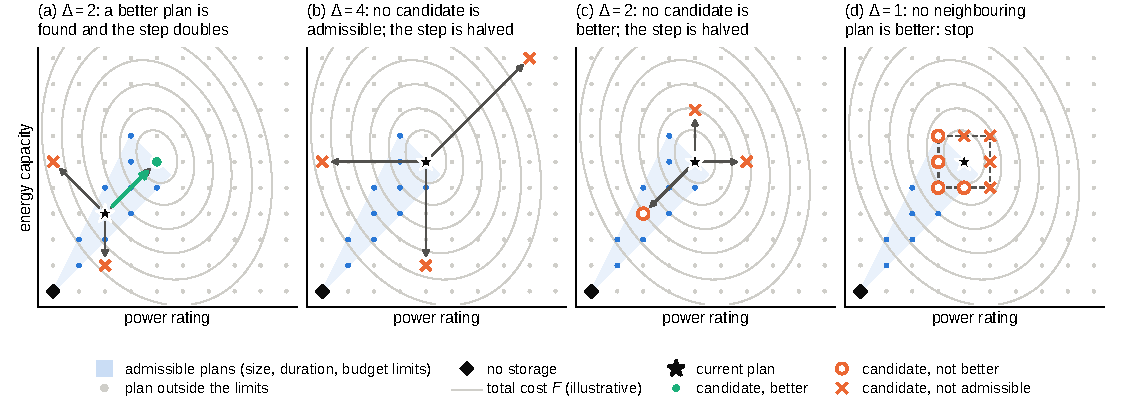
\includegraphics[width=1.00\textwidth]{fig_search_generic.pdf}
    \caption{\textcolor{blue}{Illustration of the discrete planning search in two dimensions. Shading identifies admissible plans; contours show an illustrative objective unavailable to the search. (a) An improving candidate is accepted and the poll size increases. (b--c) Unsuccessful polls reduce the poll size. (d) A completed unit poll finds no improvement beyond the acceptance threshold, and the search terminates.}}
    \label{fig:search_generic}
\end{figure}

\textcolor{blue}{
    The planning layer is a mesh adaptive direct search (MADS) on granular variables~\cite{audet_dennis_2006,audet_granular_2019}, which handles the discrete sizes of storage investments directly.
    Algorithm~\ref{alg:shared_ess_planning_mads} details the proposed method. Its decision vector holds, for each interface node, one converter rating and one energy capacity in multiples of $\Delta^S$ and $\Delta^E$, together with a single investment year at which all selected capacity is installed.
    The master problem of Subsection~\ref{subsec:master} is more general: it admits a different installation year per node and capacity added in stages at the same node. Those degrees of freedom were not searched in this study.
}

\begin{algorithm}[htbp!]
    \caption{\textcolor{blue}{Derivative-free shared-ESS planning search.}}
    \label{alg:shared_ess_planning_mads}
    \DontPrintSemicolon
    \KwIn{Lattice and admissibility conditions \eqref{eq:master_rated_s}--\eqref{eq:master_budget}; $\Delta_0$, $N^{\max}$, $\sigma_Q$; poll variant; cache $\mathcal{C}$.}
    \KwOut{Incumbent plan $\boldsymbol{x}^{\star}$ and the scope of its final unit poll.}
    $\boldsymbol{z} \in \mathbb{Z}^{2|E^S|+1}$: the lattice coordinates of $\boldsymbol{x}$ and the investment year; admissibility checked in closed form\;
    $\boldsymbol{x}^{\text{inc}} \gets \arg\min F$ over the certified, budget-feasible points of $\mathcal{C}$ ($\boldsymbol{x} = \boldsymbol{0}$ included; ties to the lower investment); $\Delta \gets \Delta_0$; $N \gets 0$\;
    \While{polls remain and a poll can be launched}{
        \uIf{variant A}{
            $\mathcal{P} \gets$ the $n+1$ OrthoMADS points $\boldsymbol{z}^{\text{inc}} + \Delta \boldsymbol{v}$, inadmissible ones dropped; \lIf{$\Delta = 1$}{$\mathcal{P} \gets \mathcal{P} \cup$ every admissible unit neighbour of $\boldsymbol{z}^{\text{inc}}$ ($\infty$-norm box)}
        }
        \Else(variant B, $\Delta = 1$ throughout){
            $\mathcal{P} \gets$ the $2n$ OrthoMADS points $\boldsymbol{z}^{\text{inc}} \pm \boldsymbol{v}$, each inadmissible point snapped to the nearest admissible point of the unit frame; \lIf{fewer than $n+1$ distinct points}{add every admissible unit neighbour}
        }
        \lIf{$|\mathcal{P}|$ exceeds the completion cap, or the new points of $\mathcal{P}$ exceed $N^{\max} - N$}{\textbf{stop}}
        Evaluate each new point of $\mathcal{P}$ by Algorithm~\ref{alg:operational_planning_degradation} under its production exit; record $F$, its settling bar and its exit (a failed evaluation is a barrier point, $F = +\infty$); add the records to $\mathcal{C}$; $N \gets N +$ new evaluations\;
        \eIf{some $\boldsymbol{x} \in \mathcal{P}$ has $F(\boldsymbol{x}^{\text{inc}}) - F(\boldsymbol{x}) > \max\{\text{bar}_{\boldsymbol{x}} + \text{bar}_{\text{inc}},\, \sigma_Q\}$}{
            $\boldsymbol{x}^{\text{inc}} \gets$ the best such point; $\Delta \gets 2\Delta$ (variant A) or $1$ (variant B)\;
        }{
            \lIf{$\Delta = 1$}{\textbf{terminate}: no evaluated unit neighbour improves $\boldsymbol{x}^{\text{inc}}$}
            $\Delta \gets \Delta/2$\;
        }
    }
    \Return{$\boldsymbol{x}^{\text{inc}}$, the poll history and the scope of the final unit poll}\;
\end{algorithm}

\textcolor{blue}{
    At each iteration the search evaluates a poll, a set of candidate plans around the current plan (the incumbent) at the current poll size $\Delta$, along a positive spanning set of directions generated deterministically by the OrthoMADS rule~\cite{abramson_orthomads_2009}, either a minimal basis of $n+1$ directions (variant A) or $2n$ directions (variant B); inadmissible points are dropped and, in variant B, snapped to the nearest admissible point.
    At unit poll size variant A completes the poll with every admissible unit neighbour of the incumbent, so that a completed unsuccessful unit poll establishes that no admissible unit neighbour reduces the evaluated objective beyond the acceptance threshold (Fig.~\ref{fig:search_generic}d). Each new poll point is evaluated by the coordination procedure of Algorithm~\ref{alg:operational_planning_degradation} and a point replaces the incumbent only if it improves $F$ by more than the two evaluations’ settling bars (the largest objective step over an evaluation’s last ten cycles) and the measured resolution $\sigma_Q$ of the recourse (Section~\ref{sec:case_settings}). 
    The search terminates when no evaluated candidate in the final unit poll improves the incumbent beyond the acceptance threshold, or when a poll exceeds the completion cap or the evaluation budget is reached (Section~\ref{sec:case_settings}). Conclusions about neighbouring plans are restricted to those actually evaluated. 
    In variant A, $\Delta$ doubles after a successful poll and halves after an unsuccessful poll; variant B maintains $\Delta=1$.
}


\subsection{Master Problem}
\label{subsec:master}

\textcolor{blue}{At the master-planning level, the framework determines a single, scenario-independent multi-year investment plan for shared ESSs at TN–DN interface nodes, including siting, sizing, and staged capacity expansion. Uncertainty in future ESS investment costs is represented through a set of low, medium, and high cost trajectories. These trajectories affect the expected investment expenditure, but the physical investment decisions remain common to all scenarios and are passed directly to the operational recourse problem.}
%Under this modeling choice, the operational subproblem assesses the expected shared ESS deployment induced by the investment-cost uncertainty representation. This approximation preserves tractability while allowing the planning layer to internalize uncertain investment conditions.

\subsubsection{Objective Function}

\textcolor{blue}{The planning search seeks to minimise the expected discounted investment cost plus the evaluated expected discounted operating cost of the investment plan:}

\textcolor{blue}{
    \begin{equation}
        \min_{\boldsymbol{x}\in\mathcal{X}} F(\boldsymbol{x})
        \label{eq:master_objective}
    \end{equation}
}

\textcolor{blue}{
    \begin{equation}
        F(\boldsymbol{x}) = I(\boldsymbol{x}) + Q(\boldsymbol{x})
        \label{eq:master_objective_value}
    \end{equation}
}

\textcolor{blue}{
    The expected discounted investment cost is given by:
}

\textcolor{blue}{
    \begin{equation}
        I(\boldsymbol{x}) = \sum_{e\in E^S} \sum_{y^{\text{Inv}}\in Y} \sum_{c\in\Omega_C} \frac{\omega_c}{(1+r)^{y^{\text{Inv}}-y_0}}
        \left(
            c^{\text{Inv,S}}_{y^{\text{Inv}},c} S^{\text{Inv}}_{e,y^{\text{Inv}}}
            +
            c^{\text{Inv,E}}_{y^{\text{Inv}},c} E^{\text{Inv}}_{e,y^{\text{Inv}}}
        \right)
    \end{equation}
}

\noindent
\textcolor{blue}{
    where $c^{\text{Inv,S}}_{y^{\text{Inv}},c}$ and $c^{\text{Inv,E}}_{y^{\text{Inv}},c}$ are the unit costs of converter apparent-power rating and energy capacity in installation year $y^{\text{Inv}}$ under cost trajectory $c$.
    The variables $S^{\text{Inv}}_{e,y^{\text{Inv}}}$ and $E^{\text{Inv}}_{e,y^{\text{Inv}}}$ denote the corresponding capacity additions at node $e$. Investment expenditure is weighted by the trajectory probabilities $\omega_c$ and discounted to the initial year $y_0$ at rate $r$.
}

\textcolor{blue}{
    The investment decisions are common to all cost trajectories: uncertainty affects the expected expenditure, rather than producing scenario-dependent physical capacities.
    The term $Q(\boldsymbol{x})$ is the expected discounted operating cost returned by the operational evaluation, as defined in Subsection~\ref{subsubsec:certification}.
}

\subsubsection{Total Rated Power and Energy Capacity}

\textcolor{blue}{
    For each node $e$ and representative year $y$, the set of
    installation years whose cohorts remain active is:
    \begin{equation}
        \mathcal{Y}^{\text{Act}}_{e,y}
        =
        \left\{
            y^{\text{Inv}}\in Y :
            y^{\text{Inv}}\le y,\quad
            y-y^{\text{Inv}}<
            T^{\text{Cal}}_{e,y^{\text{Inv}}}
        \right\}.
        \label{eq:active_cohorts}
    \end{equation}
    An installation contributes only after it has been made
    and before its calendar lifetime expires.
}

\textcolor{blue}{
    The total rated converter apparent power and energy capacity at node $e$ in representative year $y$ are obtained by summing the capacity additions whose calendar lifetimes have not expired ($\forall e\in E^S$, $\forall y\in Y$):
}

\textcolor{blue}{
    \begin{equation}
        S^{\text{Rated}}_{e,y}
        =
        \sum_{y^{\text{Inv}}\in\mathcal{Y}^{\text{Act}}_{e,y}}
        S^{\text{Inv}}_{e,y^{\text{Inv}}}
        \label{eq:master_rated_s}
    \end{equation}
}

\textcolor{blue}{
    \begin{equation}
        E^{\text{Rated}}_{e,y}
        =
        \sum_{y^{\text{Inv}}\in\mathcal{Y}^{\text{Act}}_{e,y}}
        E^{\text{Inv}}_{e,y^{\text{Inv}}}
    \end{equation}
}

\noindent
\textcolor{blue}{
    where 
    $S^{\text{Inv}}_{e,y^{\text{Inv}}}$ and $E^{\text{Inv}}_{e,y^{\text{Inv}}}$ denote the converter apparent-power rating and energy capacity installed at node $e$ in year $y^{\text{Inv}}$, and
    $T^{\text{Cal}}_{e,y^{\text{Inv}}}$ is the calendar lifetime of that installation. 
    Rated capacities represent installed nameplate capacities; the reduction in available energy due to degradation is accounted for in the operational subproblem.
}

\textcolor{blue}{
    Capacity additions are restricted to non-negative integer multiples of $\Delta^S$ and $\Delta^E$, respectively, defining the discrete investment space.
}

\subsubsection{Maximum Installable Capacity}

The total rated energy capacity at each interface node is bounded by the maximum installable capacity, reflecting physical, spatial or technical constraints at the substation ($\forall e\in E^S$, $\forall y\in Y$):

\begin{equation}
    E_{e,y}^{\text{Rated}} \leq E^{\text{Max}}_{e,y}
\end{equation}

\noindent
\textcolor{blue}{
    where $E^{\text{Max}}_{e,y}$ is the maximum total rated energy capacity permitted at node $e$ in representative year $y$.
}

\subsubsection{\textcolor{blue}{Energy-to-Converter-Rating Ratio}}

\textcolor{blue}{
    Each capacity addition is subject to bounds on the ratio of rated energy capacity to converter apparent-power rating ($\forall e\in E^S$, $\forall y^{\text{Inv}}\in Y$):
}

\textcolor{blue}{
    \begin{equation}
        \phi^{\text{Min}}_e S^{\text{Inv}}_{e,y^{\text{Inv}}} \leq 
        E^{\text{Inv}}_{e,y^{\text{Inv}}} \leq 
        \phi^{\text{Max}}_e S^{\text{Inv}}_{e,y^{\text{Inv}}}
        \label{eq:master_duration}
    \end{equation}
}

\noindent
\textcolor{blue}{
    where $\phi^{\text{Min}}_e$ and $\phi^{\text{Max}}_e$ are the minimum and maximum admissible energy-to-converter-rating ratios, expressed in MWh/MVA. These bounds constrain the relative sizing of the battery and converter.
}

\textcolor{blue}{
    At unity power factor, the converter's apparent-power rating corresponds numerically to its maximum active-power output. The ratio is therefore used as a nominal duration indicator. It does not represent the achievable discharge duration, which also depends on usable energy, discharge efficiency, degradation and reactive-power provision.
}

\subsubsection{\textcolor{blue}{Expected Discounted Investment-Expenditure Limit}}

\textcolor{blue}{
    The expected discounted expenditure of the investment plan is bounded by the planning budget:
}

\begin{equation}
    I(\boldsymbol{x}) \leq c^{\text{Inv}}
    \label{eq:master_budget}
\end{equation}

\noindent
\textcolor{blue}{
    where 
    $c^{\text{Inv}}$ is the budget for expected investment expenditure discounted to the initial year $y_0$.
    The constraint applies to the probability-weighted expenditure over the investment-cost trajectories. It does not require expenditure under every individual trajectory to remain within the budget.
}

\textcolor{blue}{
    Together, \eqref{eq:master_rated_s}--\eqref{eq:master_budget} and the integrality of the investments define the admissible set $\mathcal{X}$, a finite set of discrete plans (the shaded region of Fig.~\ref{fig:search_generic}). 
}

\subsubsection{\textcolor{blue}{Coupling Between Planning and Operational Recourse}}

\textcolor{blue}{
    For each candidate plan, the scenario-independent capacity additions $S^{\text{Inv}}_{e,y^{\text{Inv}}}$ and $E^{\text{Inv}}_{e,y^{\text{Inv}}}$ are held fixed in the operational subproblem, where they enter as the parameters $\hat{S}^{\text{Inv}}_{e,y^{\text{Inv}}}$ and $\hat{E}^{\text{Inv}}_{e,y^{\text{Inv}}}$ of Subsection~\ref{subsubsec:capacity}. The resulting evaluated operating cost $Q(\boldsymbol{x})$, together with its stopping status and numerical diagnostics, is returned to the planning search. The evaluation and numerical acceptance criteria are described in Subsection~\ref{subsubsec:certification}.
}

\subsubsection{\textcolor{blue}{Recourse Evaluation and Certification}}
\label{subsubsec:certification}

\textcolor{blue}{
    The evaluated expected discounted operating cost of a fixed investment plan is obtained by aggregating the daily costs returned by the TSO--DSO coordination procedure:
}

\textcolor{blue}{
    \begin{equation}
        Q(\boldsymbol{x}) =
        \sum_{y \in Y} \frac{Y_y}{(1+r)^{y-y_0}}
        \sum_{d \in D} D_d
        \sum_{m \in \Omega_M} \sum_{o \in \Omega_O} \omega_m \, \omega_o \,
        C^{\text{Op}}_{y,d,m,o}(\boldsymbol{x})
        \label{eq:recourse_value}
    \end{equation}
}

\noindent
\textcolor{blue}{
    where 
    $C^{\text{Op}}_{y,d,m,o}(\boldsymbol{x})$ is the evaluated daily operating cost for representative year $y$, day $d$, market scenario $m$ and operation scenario $o$. It includes TN generation costs, activated DN flexibility, load curtailment, and penalties on storage energy-closure and network-feasibility slacks. In the multi-scenario instance, it also includes the commitment charge and the deviation component of interface settlement (Subsection~\ref{subsubsec:commitment}).
}

\textcolor{blue}{
    The contracted component of interface settlement is excluded as a transfer between operators. Storage-agent and solver regularisation terms are also excluded. Renewable curtailment is assigned no cost and is reported separately as curtailed energy.
}

\textcolor{blue}{
    The weights $Y_y$ and $D_d$ are the numbers of calendar years and days represented by $y$ and $d$, respectively. Operating costs are discounted to $y_0$ using the representative year $y$.
}

\textcolor{blue}{
    \paragraph{Stopping and certification} 
    No convergence guarantee is available for consensus ADMM on a nonconvex recourse of this kind; each evaluation is therefore stopped by an explicit rule.
    Each recourse evaluation runs the coordination procedure of \ref{app:admm_updated} until the primal and dual residuals of every consensus channel pass the absolute-plus-relative test of Boyd et al.~\cite{boyd_admm_2011} in a cycle in which every local solve is successful. On a nonconvex recourse this does not imply that the objective has settled (Subsection~\ref{subsec:res_certification}), so the residual pass only opens a certifying regime, with the coordination settings held fixed, in which the evaluation continues until the trajectory of its objective shows that it has settled. On the oscillatory branch, the oscillation must have a measured period, must not be growing (the growth test) and must stay within a tolerance $\tau$ over that period; the operators' remaining disagreement at the interface, priced at the expected wholesale price, must be within $\tau/2$ (the gap clause); and the evidence must come from cleanly solved cycles. An objective that descends without oscillating is certified instead on a monotone branch that bounds its remaining descent, under the same gap clause and clean-evidence condition. The rule is stated in full in \ref{app:admm_updated_certification}. An evaluation that does not certify within its cycle cap is reported in an uncertified form, with its consensus gap at the cap and its settling slack, the movement of the objective since the certification cycle of its earlier, residual-based run.
}

\textcolor{blue}{
    \paragraph{Resolution} The tolerance $\tau$ is set from the value resolution $\delta_R$ the study is to claim: $\tau = \delta_R \mathcal{V}/4$, with $\mathcal{V}$ a reference storage value, so that a ratio of two values --- four evaluations, each in error by at most $\tau$ --- is resolved to $\delta_R$. The rule bounds the stopping error of each evaluation at about $\tau$, not well inside it (Subsection~\ref{subsec:res_certification}); the values used in the case study are given in Section~\ref{sec:case_settings}.
}

\textcolor{blue}{
    \paragraph{Determinacy} A difference between two certified evaluations is called determinate when it is at least $\max\{3\,b, 2\tau\}$, where $b$ is the larger of the two certification bands (the range of the objective over the certifying window). A difference involving uncertified evaluations is determinate only if it exceeds three times the largest of their consensus gaps and settling slacks, in both gross and gap-corrected terms (the objective plus the priced gap). Every planning statement in this paper is a pairwise comparison of evaluations with this threshold stated; smaller differences are ties, reported as ``within resolution''. The master search of Algorithm~\ref{alg:shared_ess_planning_mads} accepted its poll points by the resolution rule stated there; every incumbent it proposed was re-evaluated under this rule before being reported. What is certified is each evaluation, not the plan: the method claims no optimality certificate for the nonconvex recourse, and the bands, gaps and slacks of every single-scenario evaluation used in a reported comparison are tabulated in~\ref{app:results}; the multi-scenario evaluations, stopped by the production exit, carry the resolution stated with them in Table~\ref{tab:res_multiscenario}.
}

\subsection{Subproblem}
\label{subsec:subproblem}

\textcolor{blue}{
    For a fixed investment plan, coordinated operation is decomposed into TSO and DSO network subproblems for each representative year--day pair, together with one shared-ESS subproblem per interface node. Each shared-ESS subproblem spans all representative years and days, enforcing the degradation dynamics that couple operation across the planning horizon. The subproblems are coordinated through ADMM, allowing each system operator to retain its network model and operating data locally while exchanging the quantities required for coordination.
}

\subsubsection{Shared ESS Operation Subproblem}

\textcolor{blue}{
    The ADMM-based TSO--DSO coordination framework introduced in~\cite{simoes_2023} is extended with shared-ESS agents that track state of health and available energy capacity across representative years. The local optimisation problems are detailed in \ref{app:admm_updated_implementation}, and the coordination procedure is summarised in Algorithm~\ref{alg:operational_planning_degradation} (\ref{app:admm_updated_algorithm}).
}

\textcolor{blue}{
    For notational compactness, the scenario indices are omitted from the detailed TSO, DSO and shared-ESS formulations. Each network block model holds every scenario of its block jointly, with the objective weighted by the scenario probabilities; within the block the storage schedule and the TSO's interface exchange are scenario-free, and the storage agent carries no scenario index at all (Subsection~\ref{subsubsec:commitment}).
}

\textcolor{blue}{
    The net storage schedule --- active and reactive power at the interface node in every hour --- is a consensus variable between the operators' network models and the shared-ESS agent: the network models carry the state-of-charge dynamics and the converter limits, and the agent carries the ageing chain that links the representative years. 
    The network models and the shared-ESS agent maintain separate charging and discharging variables. The network models impose a relaxed complementarity constraint, while the shared-ESS agent uses a throughput regularisation term. Cell degradation is computed from the agent's charging and discharging variables.
}

\subsubsection{\textcolor{blue}{Installed and Available Capacity}}
\label{subsubsec:capacity}

\textcolor{blue}{
    Each capacity addition at node $e$ in installation year $y^{\text{Inv}}$ forms an investment cohort, whose ratings are the fixed additions $\hat{S}^{\text{Inv}}_{e,y^{\text{Inv}}}$ and $\hat{E}^{\text{Inv}}_{e,y^{\text{Inv}}}$ of the candidate plan ($\forall e\in E^S$, $\forall y\in Y$, $\forall y^{\text{Inv}}\in\mathcal{Y}^{\text{Act}}_{e,y}$):
}

\textcolor{blue}{
    \begin{equation}
        S^{\text{Rated,Unit}}_{e,y^\text{Inv},y} = \hat{S}^{\text{Inv}}_{e,y^\text{Inv}}
        \label{eq:cohort_rated}
    \end{equation}
}

\textcolor{blue}{
    \begin{equation}
        E^{\text{Rated,Unit}}_{e,y^\text{Inv},y} = \hat{E}^{\text{Inv}}_{e,y^\text{Inv}}
        \label{eq:cohort_rated_energy}
    \end{equation}
}

\textcolor{blue}{
    The model keeps each cohort's converter rating unchanged over its calendar lifetime, while its available energy decreases with its state of health, evaluated at the end of the block represented by year $y$. This gives a conservative capacity estimate within the block; evaluation at the block midpoint is examined in Subsection~\ref{subsec:res_degradation}:
}

\textcolor{blue}{
    \begin{equation}
        S^{\text{Av,Unit}}_{e,y^\text{Inv},y} = S^{\text{Rated,Unit}}_{e,y^\text{Inv},y}
        \label{eq:cohort_available}
    \end{equation}
}

\textcolor{blue}{
    \begin{equation}
        E^{\text{Av,Unit}}_{e,y^\text{Inv},y} = E^{\text{Rated,Unit}}_{e,y^\text{Inv},y}\, SoH_{e,y^\text{Inv},y}
        \label{eq:cohort_available_energy}
    \end{equation}
}

\textcolor{blue}{
    The capacities seen by the network models in year $y$ are the sums over the active cohorts ($\forall e \in E^S$, $\forall y \in Y$):
}

\textcolor{blue}{
    \begin{equation}
        S^{\text{Av}}_{e,y} = \sum_{y^{\text{Inv}}\in\mathcal{Y}^{\text{Act}}_{e,y}} S^{\text{Av,Unit}}_{e,y^{\text{Inv}},y}
        \label{eq:available_power}
    \end{equation}
}

\textcolor{blue}{
    \begin{equation}
        E^{\text{Av}}_{e,y} = \sum_{y^{\text{Inv}}\in\mathcal{Y}^{\text{Act}}_{e,y}} E^{\text{Av,Unit}}_{e,y^{\text{Inv}},y}
        \label{eq:available_capacity}
    \end{equation}
}

\textcolor{blue}{
    The storage agent publishes $S^{\text{Av}}_{e,y}$ and $E^{\text{Av}}_{e,y}$ to every network block at each
    coordination cycle; this is the path by which degradation reaches the operating decisions.
}

\subsubsection{\textcolor{blue}{Storage Operation in the Network Models}}
\label{subsubsec:network_storage}

\textcolor{blue}{
    In each network model containing shared ESS $e$, charging and discharging are represented by non-negative active-power variables $P^{\text{Ch}}_{e,y,d,t}$ and $P^{\text{Dch}}_{e,y,d,t}$.
    The net active power follows a consumption convention: positive values denote charging and negative values denote discharging. Reactive power is represented separately by $Q^{\text{E}}_{e,y,d,t}$ ($\forall e\in E^S$, $\forall y\in Y$, $\forall d\in D$, $\forall t\in T$):
}

\textcolor{blue}{
    \begin{equation}
        P^{\text{E}}_{e,y,d,t}
        =
        P^{\text{Ch}}_{e,y,d,t}
        -
        P^{\text{Dch}}_{e,y,d,t}
        \label{eq:storage_net_active_power}
    \end{equation}
}

\textcolor{blue}{
    The variable $E^{\text{SoC}}_{e,y,d,t}$ denotes stored energy at the end of time interval $t$, rather than a fractional state of charge. Starting from the initial stored energy $E^{\text{SoC}}_{e,y,d,0}$, its evolution is:
}

\textcolor{blue}{
    \begin{equation}
        E^{\text{SoC}}_{e,y,d,t} = E^{\text{SoC}}_{e,y,d,t-1}
        + \Delta t \left( \eta^{\text{Ch}}_e P^{\text{Ch}}_{e,y,d,t} - \frac{P^{\text{Dch}}_{e,y,d,t}}{\eta^{\text{Dch}}_e} \right)
        \label{eq:soc_recursion}
    \end{equation}
}

\noindent
\textcolor{blue}{
    where $\Delta t$ is the duration of each time interval, and $\eta^{\text{Ch}}_e$ and $\eta^{\text{Dch}}_e$ are the charging and discharging efficiencies. Charging and discharging powers are measured on the network side of the converter; the efficiency factors account for the corresponding changes in stored energy.
}

\textcolor{blue}{
    Stored energy is bounded by the admissible state-of-charge window, expressed as fractions of the available energy capacity:
}

\textcolor{blue}{
    \begin{equation}
        SoC^{\text{Min}}_e E^{\text{Av}}_{e,y}
        \le E^{\text{SoC}}_{e,y,d,t}
        \le SoC^{\text{Max}}_e E^{\text{Av}}_{e,y}
        \label{eq:soc_limits}
    \end{equation}
}

\noindent
\textcolor{blue}{
    where the parameters $SoC^{\text{Min}}_e$, $SoC^{\text{Max}}_e$ and $SoC^0_e$ specify the minimum, maximum and initial fractional states of charge.
}

\textcolor{blue}{
    Each representative day starts at the prescribed fractional state of charge $SoC^0_e$:
}

\textcolor{blue}{
    \begin{equation}
        E^{\text{SoC}}_{e,y,d,0}
        =
        SoC^0_e E^{\text{Av}}_{e,y}
        \label{eq:soc_initial}
    \end{equation}
}

\textcolor{blue}{
    At the end of the day, stored energy returns to its initial value up to non-negative closure slacks:
}

\textcolor{blue}{
    \begin{equation}
        E^{\text{SoC}}_{e,y,d,|T|}
        =
        E^{\text{SoC}}_{e,y,d,0}
        + s^+_{e,y,d} - s^-_{e,y,d}
        \label{eq:soc_closure}
    \end{equation}
}

\textcolor{blue}{
    The slacks permit a bounded deviation from exact daily closure and are penalised at $c^{\text{Cl}}$ per MWh in the network objectives:
}

\textcolor{blue}{
    \begin{equation}
        0 \le s^\pm_{e,y,d}
        \le \varepsilon^{\text{Cl}} E^{\text{Av}}_{e,y}
        \label{eq:soc_closure_slack}
    \end{equation}
}

\textcolor{blue}{
    No energy is carried between representative days.    
    In the multi-scenario instance, the shared-ESS schedule is common to all market and operation scenarios within each representative year--day block. It therefore represents a day-ahead commitment, as described in Subsection~\ref{subsubsec:commitment}.    
}

\textcolor{blue}{
    The sum of charging and discharging active powers is limited by the available converter rating:
}

\textcolor{blue}{
    \begin{equation}
        P^{\text{Ch}}_{e,y,d,t}
        + P^{\text{Dch}}_{e,y,d,t}
        \le S^{\text{Av}}_{e,y}
        \label{eq:storage_active_power_limit}
    \end{equation}
}

\textcolor{blue}{
    Net active power and reactive power share the converter's apparent-power capability:
}

\textcolor{blue}{
    \begin{equation}
        \left(P^{\text{E}}_{e,y,d,t}\right)^2
        + \left(Q^{\text{E}}_{e,y,d,t}\right)^2
        \le \left(S^{\text{Av}}_{e,y}\right)^2
        \label{eq:converter_capability}
    \end{equation}
}

\textcolor{blue}{
    In this model, reactive-power provision affects converter utilisation but does not directly affect stored energy or cell degradation.
}

\textcolor{blue}{Simultaneous charging and discharging is restricted by a normalised complementarity condition relaxed with tolerance $\varepsilon^{\text{C}}$:}

\textcolor{blue}{
    \begin{equation}
        \frac{P^{\text{Ch}}_{e,y,d,t}}{S^{\text{Av}}_{e,y}} \; \frac{P^{\text{Dch}}_{e,y,d,t}}{S^{\text{Av}}_{e,y}} \le \varepsilon^{\text{C}}
        \label{eq:network_complementarity}
    \end{equation}
}

\textcolor{blue}{
    The operating parameters are specified in Section~\ref{sec:case_ess_params}.
    At every certificate used in a reported comparison, and at both multi-scenario evaluations, both daily closure slacks sat at their lower bound to within the solver's bound relaxation ($10^{-6}$~MWh per slack); in the superseded evaluation~16 of Table~\ref{tab:appE_evaluations} their sum reached $1.8 \times 10^{-6}$~MWh, $5 \times 10^{-6}$ of the available energy. Without storage the closure row is deactivated and its slacks are fixed at zero.
}

\subsubsection{\textcolor{blue}{Degradation Chain of the Shared-ESS Agent}}

\textcolor{blue}{The shared-ESS agent holds its own copy of the storage schedule, in consensus with the network models' copies through the ADMM channel of \ref{app:admm_updated}, and ages the cohorts with it. Its net active power at node $e$ is the sum of the cohorts' charging and discharging powers, up to a slack pair that is penalised in its objective and was at its lower bound at every certified point ($\forall e$, $y$, $d$, $t$):}

\textcolor{blue}{
    \begin{equation}
        P^{\text{Net}}_{e,y,d,t} = \sum_{y^\text{Inv}} \left( P^{\text{Ch}}_{e,y^\text{Inv},y,d,t} - P^{\text{Dch}}_{e,y^\text{Inv},y,d,t} \right)
        + \sigma^{+}_{e,y,d,t} - \sigma^{-}_{e,y,d,t}, \qquad \sigma^{\pm}_{e,y,d,t} \ge 0
        \label{eq:esso_net_power}
    \end{equation}
}

\textcolor{blue}{When several cohorts are alive at a node, the net schedule is allocated to them in proportion to their rated energy --- a homogeneous-fleet approximation in which all cohorts at a node cycle at the same depth; every plan reported in this paper has a single cohort per node, for which the allocation is vacuous ($\forall e$, $y^\text{Inv}$, $y$, $d$, $t$):}

\textcolor{blue}{
    \begin{equation}
        P^{\text{Ch}}_{e,y^\text{Inv},y,d,t} - P^{\text{Dch}}_{e,y^\text{Inv},y,d,t} =
        \frac{E^{\text{Rated,Unit}}_{e,y^\text{Inv},y}}{\sum_{y'} E^{\text{Rated,Unit}}_{e,y',y}}
        \sum_{y''} \left( P^{\text{Ch}}_{e,y'',y,d,t} - P^{\text{Dch}}_{e,y'',y,d,t} \right)
        \label{eq:cohort_allocation}
    \end{equation}
}

\textcolor{blue}{Ageing is driven by the energy that crosses the cells, not by the apparent power at the
converter: the average daily cell-side throughput of a cohort in representative year $y$ is}

\textcolor{blue}{
    \begin{equation}
        \bar{E}^{\text{Cell}}_{e,y^\text{Inv},y} =
        \sum_{d \in D} \frac{D_d}{365} \sum_{t \in T} \Delta t
        \left(
            \eta^{\text{Ch}}_e P^{\text{Ch}}_{e,y^\text{Inv},y,d,t}
            +
            \frac{P^{\text{Dch}}_{e,y^\text{Inv},y,d,t}}{\eta^{\text{Dch}}_e}
        \right)
        \label{eq:cell_throughput}
    \end{equation}
}

\textcolor{blue}{and the fractional cycling loss accumulated over the $Y_y$ calendar years of the block is}

\textcolor{blue}{
    \begin{equation}
        D_{e,y^\text{Inv},y} =
        \frac{365 \, Y_y \, \bar{E}^{\text{Cell}}_{e,y^\text{Inv},y}}
             {2 \, k_e \, E^{\text{Rated,Unit}}_{e,y^\text{Inv},y}}
        \label{eq:cycling_loss}
    \end{equation}
}

\noindent
\textcolor{blue}{where $k_e$ is the effective cycle life of the technology: $2 E^{\text{Rated,Unit}}$ is the throughput of one full cycle, so $D$ counts equivalent full cycles against $k_e$. The state of health then follows a continuous-compounding chain with a calendar retention factor $\phi^{\text{Cal}}_e$ per calendar year ($\forall e$, $y^\text{Inv}$, $y$):}

\textcolor{blue}{
    \begin{equation}
        SoH_{e,y^\text{Inv},y} = SoH_{e,y^\text{Inv},y-1} \, \exp\!\left(-D_{e,y^\text{Inv},y}\right)
        \left(\phi^{\text{Cal}}_e\right)^{Y_y},
        \qquad SoH_{e,y^\text{Inv},y^\text{Inv}-1} = 1
        \label{eq:soh_chain}
    \end{equation}
}

\textcolor{blue}{
    \begin{equation}
        SoH_{e,y^\text{Inv},y} \ge SoH^{\text{Min}}_e
        \label{eq:soh_floor}
    \end{equation}
}

\textcolor{blue}{The constant $k_e$ is calibrated from a datasheet statement of $N^{\text{DS}}$ cycles at depth of discharge $\delta^{\text{DS}}$ to a retention $R^{\text{DS}}$ of the rated capacity: with \eqref{eq:cycling_loss}--\eqref{eq:soh_chain} and no calendar term, those cycles give $SoH = \exp(-\delta^{\text{DS}} N^{\text{DS}} / k_e) = R^{\text{DS}}$, hence}

\textcolor{blue}{
    \begin{equation}
        k_e = \frac{\delta^{\text{DS}} N^{\text{DS}}}{-\ln R^{\text{DS}}}
        \label{eq:cycle_life_calibration}
    \end{equation}
}

\noindent
\textcolor{blue}{
    The calibrations used, the calendar retention and the end-of-life floor $SoH^{\text{Min}}_e$ are given in Section~\ref{sec:case_ess_params}. The floor is the only intertemporal trade-off enforced in operation: no explicit cycling cost is charged, because a shared asset that has been paid for carries no operating cost of its own; degradation is tracked and propagated, and its economic effect appears through the available energy of later years and through the floor. 
    Equations \eqref{eq:cycling_loss} and \eqref{eq:soh_floor} are linear; \eqref{eq:soh_chain}, the available-energy product in \eqref{eq:cohort_available_energy} and the converter circle are the agent's nonlinear rows.
}

\textcolor{blue}{
    The agent has no economic objective, and its objective value is not part of $Q(\boldsymbol{x})$. Within the coordination procedure it minimizes its consensus terms, a penalty on the slack pair of \eqref{eq:esso_net_power} and a small linear penalty on its charging and discharging powers, and it enforces the converter capability inequality on its aggregate schedule (\ref{app:admm_updated_implementation}). The linear penalty makes simultaneous charging and discharging non-optimal, so complementarity in the agent follows from the problem structure and needs no nonconvex constraint.
}

\textcolor{blue}{
    The degradation calculated by the proposed model corresponds to the total utilization of the shared ESS resulting from coordinated TSO–DSO operation. During the coordination procedure, the participating system operators communicate their active- and reactive-power requests, which are reconciled with the physical and degradation constraints of the shared ESS. Consequently, the final ESS schedule represents a jointly optimized operating trajectory rather than the superposition of independently determined TSO and DSO schedules. The resulting degradation therefore cannot be uniquely attributed to either the TSO or the DSOs without introducing an additional benefit- or cost-allocation mechanism.
}

\subsubsection{\textcolor{blue}{Day-Ahead Commitment under Operation Scenarios}}
\label{subsubsec:commitment}

\textcolor{blue}{
    In the multi-scenario instance every scenario $s = (m, o)$ --- a market scenario $m \in \Omega_M$ and an operation scenario $o \in \Omega_O$ of load and RES generation, with probability $\omega_s = \omega_m \omega_o$ --- is held inside every network block, while the interface schedule committed to the TSO is scenario-free by construction in the TSO model, which re-dispatches its own network per scenario against it, and may be deviated from on the DSO side. 
    Each DSO carries a day-ahead expectation of its interface flow and is charged for deviating from it. With $P^{\text{I}}_{i,s,t}$ the interface active power of DSO $i$ in scenario $s$ and hour $t$ (likewise $Q^{\text{I}}$), the expectation and the deviations are ($\forall i$, $s$, $t$):
}

\textcolor{blue}{
    \begin{equation}
        \bar{P}^{\text{I}}_{i,t} = \sum_{s \in \Omega_M \times \Omega_O} \omega_s P^{\text{I}}_{i,s,t}, \qquad
        P^{\text{I}}_{i,s,t} - \bar{P}^{\text{I}}_{i,t} = d^{+}_{i,s,t} - d^{-}_{i,s,t}, \qquad d^{\pm}_{i,s,t} \ge 0
        \label{eq:commitment_deviation}
    \end{equation}
}

\noindent 
\textcolor{blue}{
    and the charge added to the DSO's objective, and hence to $C^{\text{Op}}$ in \eqref{eq:recourse_value}, is
}

\textcolor{blue}{
    \begin{equation}
        \sum_{s \in \Omega_M \times \Omega_O} \sum_{t \in T} \omega_s \, \alpha \, \bar{\pi}_t
        \left( d^{+}_{i,s,t} + d^{-}_{i,s,t} \right)
        \label{eq:commitment_charge}
    \end{equation}
}

\noindent
\textcolor{blue}{
    where $\bar{\pi}_t$ is the probability-weighted wholesale price of the hour over the market scenarios and $\alpha$ an imbalance premium, so that a deviation is priced at a fraction $\alpha$ of the energy price of the hour in which it occurs. The same term is written on the reactive interface flow with the same price, as a stated assumption. 
    The deviation energy is also settled at the scenario price: the contracted part of the interface settlement, at the committed schedule, is a transfer between operators and is excluded from $Q(\boldsymbol{x})$, while the deviation part is inside it (Subsection~\ref{subsubsec:certification}). The TSO carries no deviation term. The interface voltage carries no priced term either, being a physical state rather than a commitment; a solver-side regularisation of its dispersion is used and excluded from $Q(\boldsymbol{x})$ (\ref{app:admm_updated}).
    The storage schedule is not deviated from: it is one scenario-free variable per hour in every block (Subsection~\ref{subsubsec:network_storage}), so the committed schedule is the one that ages the cells. With a single scenario \eqref{eq:commitment_deviation}--\eqref{eq:commitment_charge} vanish identically, so the single-scenario instance is unaffected by them; the commitment is to the expectation over market and operation scenarios alike, so deviations driven by the price realization are charged like those driven by load and generation.
    The value of $\alpha$ is given in Section~\ref{sec:case_settings}.
}

% ====================================================================================================================
%                                                      CASE STUDY                                                     
% ====================================================================================================================
\section{Case Study}
\label{sec:case_studies}

The proposed framework is evaluated on an integrated transmission--distribution test system with high RES penetration and coordinated TSO--DSO operation. The test system comprises the IEEE 9-bus transmission network coupled with three Active Distribution Networks (ADNs), each derived from the IEEE 33-bus distribution test system~\cite{zimmerman_2011,ieee_case33}. A representative single-line diagram of the integrated system is shown in Figure~\ref{fig:tso_dso_coordination_cs1_network_diagram}. 
Shared ESSs can be installed at the TN--DN interface nodes corresponding to the connection points of the three ADNs. 
\textcolor{blue}{
    The 15-year planning horizon is represented in two instances. The single-scenario instance, on which the planning results of Section~\ref{sec:results} are obtained, uses three representative years, 2025, 2030 and 2035, each standing for a five-year block, with one market scenario and one operation scenario of load and RES generation. The multi-scenario instance (Subsection~\ref{subsec:res_multiscenario}) uses five representative years, 2025, 2028, 2031, 2034 and 2037, each standing for a three-year block, with three market scenarios and three operation scenarios, nine operating scenarios per representative day. In both instances each year is represented by four seasonal representative days, weighted by the numbers of days they stand for (92, 91, 91 and 91).
}

\textcolor{blue}{
    Although the planning formulation permits different installation years across nodes and staged capacity additions, the case-study search considers a single installation year common to all selected shared ESSs, with one capacity installation per node. The numerical results therefore assess siting, sizing and the common installation year within this restricted investment space; independent installation timing across nodes and staged expansion are left for future work.
}

%\begin{figure}[htbp]
%    \centering
%    \includegraphics[width=1.00\textwidth]{network_diagram.pdf}
%    \caption{Single-line diagram of the adopted test system, including the ADNs participating in the coordination procedure.}
%    \label{fig:tso_dso_coordination_cs1_network_diagram}
%\end{figure}

\begin{figure*}[htbp]
    \centering
    \subfloat[IEEE 9-bus TN and ADN connection points.]{
        \includegraphics[width=0.50\textwidth,clip]{network_diagram_ieee9.pdf}
    }
    \vspace{0.5em}
    \subfloat[IEEE 33-bus topology adopted for each ADN.]{
        \includegraphics[width=0.65\textwidth,clip]{network_diagram_ieee33.pdf}
    }
    \caption{Adopted integrated transmission–distribution test system.}
    \label{fig:tso_dso_coordination_cs1_network_diagram}
\end{figure*}

\textcolor{blue}{
    Three ESS investment-cost trajectories are considered at the planning level (Subsection~\ref{subsec:case_investment_costs}).
}
The total investment budget for shared ESS deployment is set to 1~M\euro, and the maximum installable energy capacity at each interface node is limited to 5.00~MWh. All shared ESSs are assumed to have a calendar lifetime of 15 years, and a discount rate of 2.00\% is used to compute the NPV of all cash flows.

\textcolor{blue}{
    Two kinds of comparison are used throughout Section~\ref{sec:results}. Storage plans are compared under coordinated operation with the plan without shared storage, $\boldsymbol{x} = \boldsymbol{0}$, which isolates the value of the storage investment, or with one another; and coordinated operation at the plan without storage is compared with two static arrangements of the same system under a no-reverse-flow interface rule (Subsection~\ref{sec:case_settings}), which isolates the value of coordination.
}

\subsection{Investment Costs}
\label{subsec:case_investment_costs}

To represent uncertainty in future storage costs, three investment trajectories -- low, medium, and high -- are considered, reflecting plausible cost ranges associated with technological progress and market development~\cite{nrel_ess_costs,iea_ess_2024}. The corresponding investment costs are reported in Table~\ref{tab:investment_cost}.

\begin{table}[htbp!]
    \centering
    \caption{Investment costs of shared ESSs~\cite{nrel_ess_costs}.}
    \begin{tabular}{lcc ccc}
        \toprule
        Parameter & Scn. & Prob., [\%] & 2025 & 2030 & 2035 \\ 
        \midrule
        $c^\text{Inv,S}_{y,c}$,     & 1 & 35.00\% & 214.17 & 168.72 & 153.93\\
        $\left[\text{k\euro/MVA}\right]$ & 2 & 55.00\% & 267.53 & 224.25 & 206.96\\
        ~                           & 3 & 10.00\% & 342.17 & 278.10 & 268.58\\
        \midrule
        $c^\text{Inv,E}_{y,c}$, & 1 & 35.00\% & 212.13 & 167.11 & 152.46\\
        $\left[\text{k\euro/MWh}\right]$ & 2 & 55.00\% & 264.98 & 222.12 & 204.99\\
        ~                           & 3 & 10.00\% & 338.91 & 275.45 & 266.02\\
        \bottomrule
    \end{tabular}
    \label{tab:investment_cost}
\end{table}

%By explicitly modeling multiple investment cost trajectories and their associated probabilities, the proposed planning framework accounts for investment cost uncertainty directly within the optimization process. This enables the model not only to identify the optimal \emph{siting} and \emph{sizing} of shared ESSs, but also to make informed decisions regarding the \emph{timing} of capacity deployment. 

\textcolor{blue}{
    The three trajectories enter the plan's investment cost $I(\boldsymbol{x})$ as their probability-weighted sum, which, $I$ being linear in the unit costs, equals the cost at the expected trajectory (256.32~k\euro/MVA and 253.88~k\euro/MWh in 2025). The energy-cost row corrects the submitted version, where the cost per MWh had been derived from the 4-h system cost by dividing by 5 instead of 4.
}

\subsection{Market Data}

Baseline wholesale energy prices were obtained from the Portuguese TSO platform~\cite{ren_market_platform}, whereas flexibility market prices were sourced from the ATTEST project repository~\cite{attest_project_repo}. Seasonal profiles are provided in~\ref{app:market_data}. Wholesale energy prices are assumed to increase at an average annual rate of 2.50\%, whereas flexibility market prices increase at 2.00\% per year.

\subsection{Transmission Network}

The transmission network is based on the IEEE 9-bus test system~\cite{zimmerman_2011}. To reflect increasing RES penetration over the planning horizon, installed wind and solar PV capacities vary across the representative years, as summarized in Table~\ref{tab:cs3_tn_res_generators}. This progressive growth in variable renewable generation creates evolving flexibility needs and provides a suitable setting for evaluating the timing and value of shared ESS deployment. The RES generation profiles adopted for the spring, summer, autumn, and winter representative days of the initial planning year (2025) are provided in~\ref{app:tn_description}.
\textcolor{blue}{
    Conventional generation in the TN is priced at the wholesale energy price of the scenario; no separate generator cost curves are used.
}

\begin{table}[htbp!]
    \centering
    \caption{TN installed RES capacity in each representative year.}
    \begin{tabular}{ccc ccccc}
        \toprule
        Generator   & Node  & Generator & \multicolumn{5}{c}{Installed capacity, [MW]}\\  \cmidrule{4-8}
        ID          & ID    & Type      & 2025  & 2028  & 2031  & 2034   & 2037 \\ 
        \midrule
        4 & 4 &  Wind     & 20.00 & 20.00 & 30.00 & 30.00 & 50.00\\
        5 & 6 &  Wind     & 40.00 & 40.00 & 60.00 & 60.00 & 60.00\\
        6 & 8 &  Wind     & 25.00 & 25.00 & 40.00 & 40.00 & 40.00\\
        7 & 4 &  Solar PV & 12.00 & 12.00 & 20.00 & 20.00 & 20.00\\
        8 & 6 &  Solar PV & 20.00 & 20.00 & 30.00 & 30.00 & 50.00\\
        9 & 8 &  Solar PV & 15.00 & 15.00 & 25.00 & 25.00 & 25.00\\
        \bottomrule
    \end{tabular}
    \label{tab:cs3_tn_res_generators}
\end{table}

\subsection{Active Distribution Networks}
\label{subsec:case_study_adns}

The three ADNs share the IEEE 33-bus topology but differ in RES penetration levels and growth trajectories, thereby creating heterogeneous flexibility conditions across the TN--DN interfaces. This heterogeneity allows assessment of how the value of shared ESS deployment depends on local network characteristics. Tables~\ref{tab:cs3_adn_node_5_res_generators}--\ref{tab:cs3_adn_node_9_res_generators} summarize the installed RES capacities for the ADNs connected to TN nodes 5, 7, and 9, respectively. Seasonal RES and load profiles for the base year (2025) are provided in~\ref{app:dns_description}.

\begin{table}[htbp!]
    \centering
    \caption{ADN at TN node~5: installed RES capacity in each representative year.}
    \begin{tabular}{ccc ccccc}
        \toprule
        Generator   & Node  & Generator & \multicolumn{5}{c}{Installed capacity, [MW]}\\  \cmidrule{4-8}
        ID          & ID    & Type      & 2025  & 2028  & 2031  & 2034   & 2037 \\ 
        \midrule
        2 & 6  &  Wind    & 40.00 & 40.00 & 50.00 & 50.00 & 50.00\\
        3 & 23 & Solar PV & 15.00 & 15.00 & 25.00 & 25.00 & 25.00\\
        4 & 25 & Solar PV & 20.00 & 20.00 & 20.00 & 20.00 & 30.00\\
        5 & 18 & Solar PV & 8.00  & 8.00  & 15.00 & 15.00 & 35.00\\
        \bottomrule
    \end{tabular}
    \label{tab:cs3_adn_node_5_res_generators}
\end{table}

\begin{table}[htbp!]
    \centering
    \caption{ADN at TN node~7: installed RES capacity in each representative year.}
    \begin{tabular}{ccc ccccc}
        \toprule
        Generator   & Node  & Generator & \multicolumn{5}{c}{Installed capacity, [MW]}\\  \cmidrule{4-8}
        ID          & ID    & Type      & 2025  & 2028  & 2031  & 2034   & 2037 \\ 
        \midrule
        2 & 6  & Wind     & 40.00 & 40.00 & 50.00 & 50.00 & 50.00\\
        3 & 23 & Wind     & 40.00 & 40.00 & 40.00 & 40.00 & 40.00\\
        4 & 25 & Solar PV & 10.00 & 10.00 & 20.00 & 20.00 & 20.00\\
        5 & 18 & Solar PV & 10.00 & 10.00 & 10.00 & 10.00 & 30.00\\
        \bottomrule
    \end{tabular}
    \label{tab:cs3_adn_node_7_res_generators}
\end{table}

\begin{table}[htbp!]
    \centering
    \caption{ADN at TN node~9: installed RES capacity in each representative year.}
    \begin{tabular}{ccc ccccc}
        \toprule
        Generator   & Node  & Generator & \multicolumn{5}{c}{Installed capacity, [MW]}\\  \cmidrule{4-8}
        ID          & ID    & Type      & 2025  & 2028  & 2031  & 2034   & 2037 \\ 
        \midrule
        2 & 6  & Wind     & 20.00 & 20.00 & 50.00 & 50.00 & 50.00\\
        3 & 25 & Solar PV & 30.00 & 30.00 & 30.00 & 30.00 & 30.00\\
        4 & 23 & Solar PV & 30.00 & 30.00 & 30.00 & 30.00 & 50.00\\
        5 & 18 & Solar PV & 30.00 & 30.00 & 30.00 & 30.00 & 40.00\\
        \bottomrule
    \end{tabular}
    \label{tab:cs3_adn_node_9_res_generators}
\end{table}

Within each ADN, all 32 loads are modeled as Flexible Loads (FLs), representing downstream lower-voltage networks capable of providing flexibility services. The static and flexible portions of demand are assumed to grow at average annual rates of 1.25\% and 3.00\%, respectively. The total flexible demand is allocated according to the FL ratios reported in Table~\ref{tab:cs1_ieee33_loads}. Figure~\ref{fig:cs3_adn_node_5_flexibility}, Figure~\ref{fig:cs3_adn_node_7_flexibility}, and Figure~\ref{fig:cs3_adn_node_9_flexibility} illustrate the flexible load profiles adopted for the three ADNs, respectively.

\subsection{\textcolor{blue}{Shared Energy Storage Parameters}}
\label{sec:case_ess_params}

\textcolor{blue}{
    The shared ESS is a utility-scale lithium-ion battery (the NREL utility-scale battery category~\cite{nrel_ess_costs}) with charging and discharging efficiencies $\eta^{\text{Ch}} = 0.97$ and $\eta^{\text{Dch}} = 0.96$, a usable state-of-charge window of 10--90\,\% of the available energy ($SoC^{\text{Min}} = 0.10$, $SoC^{\text{Max}} = 0.90$) and a daily initial state of 50\,\% ($SoC^{0} = 0.50$); the daily closure slack is bounded by $\varepsilon^{\text{Cl}} = 0.05$ of the available energy (plus a numerical allowance of $10^{-5}$~p.u.) and priced at  $c^{\text{Cl}} = 10^{3}$~\euro/MWh, the network complementarity tolerance is $\varepsilon^{\text{C}} = 10^{-4}$, and the calendar lifetime is $T^{\text{Cal}} = 15$~years. The agent's regularisation weight is $\varepsilon^{\text{E}} = 10^{-5}$ and its slack penalty $c^{\sigma} = 10^{3}$. Capacities are sized on the lattice $\Delta^S = 0.25$~MVA, $\Delta^E = 0.5$~MWh with durations between 2 and 4~h, at most 5~MWh per node and a budget of 1~M\euro.
}

\textcolor{blue}{
    Fig.~\ref{fig:investment_lattice} shows the resulting plans of a single node installed in 2025: twelve are admissible, the smallest being 0.25~MVA / 0.5~MWh, which is also the only admissible plan one unit step from the plan without storage. The plan without storage therefore has fourteen admissible neighbours: the smallest unit at any non-empty subset of the three nodes, installed in 2025 or 2030.
}

\begin{figure}[htbp!]
    \centering
    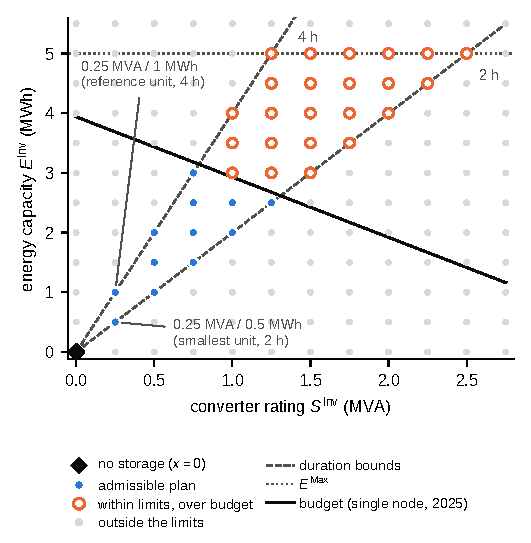
\includegraphics[width=0.55\textwidth]{fig_lattice_case.pdf}
    \caption{\textcolor{blue}{Plans of a single node installed in 2025: converter rating and energy capacity in steps of 0.25~MVA and 0.5~MWh, durations between 2 and 4~h, at most 5~MWh, and the budget at the 2025 expected unit costs. In the search the budget is shared by the three nodes.}}
    \label{fig:investment_lattice}
\end{figure}

\textcolor{blue}{
    Ageing is calibrated from datasheet cycle-life statements through \eqref{eq:cycle_life_calibration}; Table~\ref{tab:ageing_calibrations} lists the calibrations used. The baseline reads the datasheet count of 10{,}000 cycles at 80\,\% depth of discharge as cycles to 80\,\% retention ($k = 35{,}851$) and adds a calendar retention of $\phi^{\text{Cal}} = 0.985$ per year (80\,\% retention over the 15-year calendar life without cycling); the end-of-life floor is $SoH^{\text{Min}} = 0.70$. The other rows are the sensitivities of Subsection~\ref{subsec:res_degradation}: the same count without calendar fade; the same count read as cycles to 50\,\% retention, evaluated at the end of the block or at its midpoint; a second datasheet of 8{,}000 full cycles to 70\,\% retention; no ageing; and the baseline with a 0.50 floor.
}

\begin{table}[htbp!]
    \centering
    \caption{\textcolor{blue}{Ageing calibrations. $(N^{\text{DS}}, \delta^{\text{DS}}, R^{\text{DS}})$: datasheet cycles,
    depth of discharge and retention; $k_e$ from \eqref{eq:cycle_life_calibration}; SoH point: the state of health
    that sets a block's available energy (end of block, or its midpoint). $^{a}$~entered as 10\,000 cycles at 0.80 depth of discharge, the same product $N^{\text{DS}} \delta^{\text{DS}}$, which is all \eqref{eq:cycle_life_calibration} uses.}}
    \footnotesize\setlength{\tabcolsep}{4pt}
    \begin{tabular}{l c r c c c}
        \toprule
        Calibration & $(N^{\text{DS}}, \delta^{\text{DS}}, R^{\text{DS}})$ & $k_e$ & $\phi^{\text{Cal}}$ & SoH point & $SoH^{\text{Min}}$ \\
        \midrule
        Baseline (cycling + calendar) & (10\,000, 0.80, 0.80) & 35\,851 & 0.985 & end & 0.70 \\
        Cycling only                  & (10\,000, 0.80, 0.80) & 35\,851 & 1.000 & end & 0.70 \\
        Retention 50\,\%              & (10\,000, 0.80, 0.50) & 11\,542 & 1.000 & end & 0.70 \\
        Retention 50\,\%, mid-block   & (10\,000, 0.80, 0.50) & 11\,542 & 1.000 & mid & 0.70 \\
        Datasheet 8\,000 cycles$^{a}$ & (8\,000, 1.00, 0.70)  & 22\,429 & 1.000 & end & 0.70 \\
        No ageing                     & ---                   & $\infty$ & 1.000 & --- & --- \\
        Baseline, 0.50 floor          & (10\,000, 0.80, 0.80) & 35\,851 & 0.985 & end & 0.50 \\
        \bottomrule
    \end{tabular}
    \label{tab:ageing_calibrations}
\end{table}
% [AUTHOR] datasheet citations for the two cycle-life statements (10,000 cycles at 0.80 DoD; 8,000 full cycles, EVE MB31) and for the
% calendar retention 0.985/yr are still to be added before submission (round 4 item 6; Addendum 80).

\subsection{\textcolor{blue}{Planning and Certification Settings}}
\label{sec:case_settings}

\textcolor{blue}{
    Every certified evaluation reported in this paper ran the coordination procedure of \ref{app:admm_updated} under one frozen configuration, listed in \ref{app:admm_updated_settings}; the three planning-search campaigns that proposed the incumbents ran on earlier states of the code, without the tight tail, and their incumbents were re-evaluated under this configuration before being reported. In the multi-scenario instance the commitment premium of Subsection~\ref{subsubsec:commitment} is $\alpha = 0.5$.
}

\textcolor{blue}{
    Certification (Subsection~\ref{subsubsec:certification}) uses $\delta_R = 0.07$ on the reference value $\mathcal{V} = 259{,}375.33$~\euro{}, the value of the reference unit in force when the rule was adopted, hence $\tau = 4{,}539.07$~\euro{}, kept frozen thereafter, and $P_{\max} = 30$ cycles;
    an evaluation continued from, or re-run on, an earlier record is capped 100 cycles after that record's stopping cycle, a fresh one at $\min\{k_0 + 109, 300\}$. The planning search (Algorithm~\ref{alg:shared_ess_planning_mads}) used $\Delta_0 = 4$ lattice units, budgets of 20 new evaluations for the two variant-A searches and 60 for the variant-B certificate, a completion cap of 30 points, and the measured resolution $\sigma_Q = 18{,}449.66$~\euro{} of the recourse.
    The search evaluations ran under the production exit (ten consecutive passing cycles, cap 500 cycles); variant B polled at unit size throughout; a run was stopped for review when a completion set exceeded the cap or when two barrier points occurred in one poll or three in all, and ran at most 60 polls; the cache of the baseline search was seeded with the single-node ladders of the initial design, including ladder points over the budget, and the caches of the two searches under the doubled flexibility price with the certified evaluations at that price, which for the variant-B run include multi-node plans installed in 2030.
}

\textcolor{blue}{
    The value of coordination (Subsection~\ref{subsec:res_coordination}) is measured against two static arrangements of the same system, each evaluated at the same plan and under a no-reverse-flow rule at every interface: a passive arrangement, in which the DNs activate no flexibility and curtail renewable generation only as the rule requires, and a price-taker arrangement, in which each DSO dispatches its network against the wholesale price alone. 
    In both, the TSO then dispatches the TN with the interface exchanges fixed at the DNs' schedules; each DN is then re-solved once at the TN's interface voltage before the TSO dispatches again. The passive DNs select their curtailment by a minimum-curtailment term of 1~\euro/MWh; every arrangement is costed with the same function $Q$ as the coordinated value (settlement excluded, that term at zero) and reported as the best of three solver starts. The benchmark is evaluated at the plan without shared storage, at the single-scenario instance.
}

% ====================================================================================================================
%                                                       RESULTS                                                       
% ====================================================================================================================

\section{Results}
\label{sec:results}

\textcolor{blue}{
    This section reports the planning results of the revised method on the single-scenario instance of Section~\ref{sec:case_studies} and, in Subsection~\ref{subsec:res_multiscenario}, on the $3 \times 3$ multi-scenario instance. 
    Every reported number is a recourse evaluation, a difference between two of them or a quantity derived from them, and its status is stated: certified, uncertified with its bar, or, at the multi-scenario instance, stopped by the production exit;
    a difference is called determinate or within resolution by the rule of Subsection~\ref{subsubsec:certification}, and an evaluation that did not certify by its cap enters a comparison in the uncertified form of that subsection, with its bar stated. The objective is the gross operational cost $Q$ of Subsection~\ref{subsubsec:certification}, with the interface settlement excluded; the value of a plan is $Q(\boldsymbol{0}) - Q(\boldsymbol{x})$, and a plan pays when its value exceeds its investment cost $I(\boldsymbol{x})$ of \eqref{eq:investment_cost_generic}. Amounts are in thousands of euro over the 15-year horizon, discounted at 2\,\% unless stated otherwise. Where a net column appears, it is net of a terminal salvage credit computed after the evaluation from each installation's remaining calendar life and terminal state of health,
}

\textcolor{blue}{
    \begin{equation}
        C^\text{Salvage}(\boldsymbol{x}) =
        \sum_{e \in E^S} \sum_{y^\text{Inv} \in Y}
        \frac{\bar{c}^{\text{Inv,E}}_{y^\text{Inv}}\, E^{\text{Inv}}_{e,y^\text{Inv}}}{(1+r)^{\,y^\text{End}-y_0}}
        \;\frac{T^\text{Rem}_{e,y^\text{Inv}}}{T^\text{Cal}_{e,y^\text{Inv}}}
        \;\frac{SoH_{e,y^\text{Inv},y^\text{End}} - SoH^{\text{Min}}_e}{1 - SoH^{\text{Min}}_e},
        \label{eq:salvage_credit}
    \end{equation}
}

\textcolor{blue}{
    \begin{equation}
        T^\text{Rem}_{e,y^\text{Inv}} = \max\left\{0,\; y^\text{Inv} + T^\text{Cal}_{e,y^\text{Inv}} - y^\text{End}\right\},
        \label{eq:salvage_remaining_life}
    \end{equation}
}

\noindent
\textcolor{blue}{
    where $\bar{c}^{\text{Inv,E}}_{y^\text{Inv}} = \sum_{c \in \Omega_C} \omega_c\, c^{\text{Inv,E}}_{y^\text{Inv},c}$ is the expected undiscounted energy cost per MWh in the installation year, $y^\text{End}$ the end of the planning horizon, $T^\text{Rem}$ the remaining calendar life of the cohort at $y^\text{End}$ and $SoH_{e,y^\text{Inv},y^\text{End}}$ its terminal state of health. The credit returns the energy part of the cohort's cost in proportion to its remaining calendar life and to its state of health above the end-of-life floor; the converter is not credited. 
    The credit is reported, not optimized: the recourse does not see it, no plan is selected for it, and the net value is $Q(\boldsymbol{0}) - Q(\boldsymbol{x}) + C^\text{Salvage}(\boldsymbol{x})$.
}

% --------------------------------------------------------------------------------------------------------------------
\subsection{\textcolor{blue}{Planning Result at the Baseline}}
\label{subsec:res_baseline}

\textcolor{blue}{
    Under the baseline assumptions, the planning search of Algorithm~\ref{alg:shared_ess_planning_mads} returned the plan without shared storage, $\boldsymbol{x}=\boldsymbol{0}$. All fourteen admissible unit neighbours of this plan were evaluated, and none reduced the total discounted cost beyond the search resolution. 
    This result establishes the absence of an improving plan within the evaluated neighbourhood; it does not establish global optimality. Table~\ref{tab:res_value_ladder} explains the economic basis of the result. The reference unit, comprising 0.25~MVA and 1~MWh installed at node~7 in 2025, provides discounted operational savings of 253.5~k\euro{} against an investment cost of 318.0~k\euro{}. Its reported cost excess over the plan without storage is therefore 64.4~k\euro{}, corresponding to 4.93 times the determinacy threshold. Even the smallest admissible unit evaluated at node~5, comprising 0.25~MVA and 0.5~MWh, increases total cost by 49.7~k\euro{}, a difference that is also determinate.
}

\begin{table}[htbp!]
    \centering
    \caption{\textcolor{blue}{Total discounted cost increase relative to the plan without shared storage for the single-scenario baseline. Investments are made in 2025 unless stated otherwise. All reported differences are determinate and exclude terminal salvage credits.}}
    \label{tab:res_value_ladder}
    \scriptsize\setlength{\tabcolsep}{3pt}
    \begin{tabular}{l c c c c c c}
        \toprule
        Node(s) & $S^{\text{Inv}}$ (MVA) & $E^{\text{Inv}}$ (MWh) & Dur.\ (h) & $F(\boldsymbol{x}) - F(\boldsymbol{0})$ (k\euro) & Threshold/bar (k\euro) & $\times$ \\
        \midrule
        5                 & 0.25 & 0.5 & 2 & 49.7  & 12.6 & 3.94  \\
        5                 & 0.25 & 1   & 4 & 58.0  & 13.2 & 4.39  \\
        7 (reference)     & 0.25 & 1   & 4 & 64.4  & 13.1 & 4.93  \\
        7                 & 0.5  & 2   & 4 & 135.5 & 13.4 & 10.13 \\
        7$^{f}$           & 0.75 & 3   & 4 & 208.3 & 12.6 & 16.49 \\
        7                 & 1    & 4   & 4 & 274.0 & 13.6 & 20.19 \\
        7$^{u}$           & 1.25 & 5   & 4 & 347.2 & 23.9 & 14.52 \\
        7                 & 0.5  & 1   & 2 & 114.1 & 12.6 & 9.03  \\
        7$^{u}$           & 1    & 2   & 2 & 231.7 & 24.2 & 9.56  \\
        7$^{u}$           & 1.5  & 3   & 2 & 361.7 & 41.4 & 8.74  \\
        7                 & 2    & 4   & 2 & 494.4 & 13.4 & 36.91 \\
        7                 & 2.5  & 5   & 2 & 616.6 & 13.4 & 45.94 \\
        9                 & 0.25 & 1   & 4 & 61.1  & 12.6 & 4.84  \\
        9                 & 0.75 & 3   & 4 & 199.1 & 13.5 & 14.78 \\
        5 and 9           & 0.25 each & 0.5 each & 2 & 102.1 & 12.6 & 8.09 \\
        5 and 7 (2030)    & 0.25 each & 0.5 each & 2 & 93.9  & 13.4 & 7.00 \\
        \bottomrule
    \end{tabular}
    \par\smallskip
    \begin{minipage}{\linewidth}
        \scriptsize
        \raggedright
        \textcolor{blue}{%
            \textit{Note:}
            $F(\boldsymbol{x})-F(\boldsymbol{0}) = I(\boldsymbol{x})-\text{value}$. Thresholds and uncertified bars follow Subsection~\ref{subsubsec:certification}; $\times$ denotes the cost difference divided by the corresponding threshold or bar. $^{u}$: uncertified evaluation. $^{f}$: flagged certificate; applying the uncertified comparison rule gives a bar of 70.7~k\euro{} and a ratio of $2.94\times$, preserving determinacy.
        }
    \end{minipage}
\end{table}

\textcolor{blue}{
    The additional comparisons in Table~\ref{tab:res_value_ladder} show that increasing capacity or distributing it across nodes does not recover the investment cost in the evaluated cases. At node~7, the cost excess increases from 64.4 to 347.2~k\euro{} as energy capacity rises from 1 to 5~MWh for the 4~h configurations, and from 114.1 to 616.6~k\euro{} for the corresponding 2~h configurations. At a given energy capacity, the latter require twice the converter rating and consequently incur a higher power-related investment cost. The evaluated two-node plans likewise remain uneconomic: the cost excess is 102.1~k\euro{} for nodes~5 and~9 in 2025 and 93.9~k\euro{} for nodes~5 and~7 in 2030. Applying the terminal salvage credit reduces the latter to 84.0~k\euro{} without changing the conclusion. These results indicate that, under the baseline cost and operating assumptions, the operational savings from the evaluated storage investments are insufficient to offset their capital expenditure. Subsection~\ref{subsec:res_breakeven} examines the conditions under which this balance changes.
}

% --------------------------------------------------------------------------------------------------------------------
\subsection{\textcolor{blue}{Break-even Conditions}}
\label{subsec:res_breakeven}

\textcolor{blue}{
    The baseline results motivate examining the investment costs and flexibility prices at which shared storage becomes economically attractive. Figure~\ref{fig:res_breakeven} and Table~\ref{tab:res_breakeven} first examine the energy-related investment cost using an affine fit, $\text{value}=a+bE+cP$, to the evaluated 2~h and 4~h configurations at node~7. For the 4~h configurations, the fitted slope gives a break-even energy-cost estimate of $e^{*}=b+c/4-p/4$, with the converter cost fixed at $p=256{,}320$~\euro/MVA. Using the six certified evaluations gives $e^{*}=183{,}080$~\euro/MWh. Including all ten evaluations, with the uncertified and flagged evaluations represented by intervals, gives a range of 171{,}310--192{,}560~\euro/MWh. Even the upper end remains 61{,}320~\euro/MWh below the baseline energy cost of 253{,}880~\euro/MWh. In relative terms, the energy cost would have to fall by 24--33\,\% for the 4~h configurations at node~7 to pay.
    Thus, the difference between the baseline cost and the estimated break-even level persists across the evaluated numerical intervals. These estimates describe the fitted capacity range and should not be interpreted as a general model of storage value.
}

\begin{figure}[htbp!]
    \centering
    \includegraphics[width=1.00\textwidth]{fig1_breakeven.pdf}
    \caption{\textcolor{blue}{Storage investment margins at node~7 in 2025 for (a) 4~h and (b) 2~h configurations, and (c) fitted break-even energy costs against the baseline cost. Circles: certified evaluations; squares: uncertified evaluations; diamond: flagged certificate treated as an interval. Thick bars show uncertified comparison bars; thin bars add $2\tau$ and define the fitting intervals. Lines show the certified-only and interval-midpoint fits.}}
    \label{fig:res_breakeven}
\end{figure}

\begin{table}[htbp!]
    \centering
    \caption{\textcolor{blue}{Estimated break-even energy cost for 4~h storage at node~7, with converter cost fixed at 256{,}320~\euro/MVA. Ranges span all corners of the fitting
    intervals; the margin is the baseline energy cost (253{,}880~\euro/MWh) minus the break-even estimate.}}
    \label{tab:res_breakeven}
    \scriptsize\setlength{\tabcolsep}{3pt}
    \begin{tabular}{l c c c c c}
        \toprule
        Fit & Intervals & $n$ certified & $e^{*}$ certified-only & $e^{*}$ banded & Margin \\
            &           &               & (\euro/MWh)            & (\euro/MWh)    & (\euro/MWh) \\
        \midrule
        Reported                 & 4 & 6 & 183{,}080 & 171{,}310--192{,}560 & 61{,}320--82{,}570 \\
        Flagged certificate kept & 3 & 7 & 182{,}700 & 173{,}490--190{,}380 & 63{,}500--80{,}390 \\
        \bottomrule
    \end{tabular}
\end{table}

\textcolor{blue}{
    Higher flexibility procurement prices increase the operational value of shared storage, as shown in Fig.~\ref{fig:res_flex_ladder} and Table~\ref{tab:res_flex_ladder}. For each price multiplier, the reference unit and the plan without storage are evaluated under the same price assumptions. The reference unit's value exceeds its investment cost by 14.2~k\euro{} at 1.75 times the base flexibility price and by 46.3~k\euro{} at twice the base price; both differences are determinate. Linear interpolation of the reported values at multipliers of 1.5 and 1.75 places break-even at approximately 1.63 times the base price. However, the evaluation at 1.5 times the base price did not satisfy the certification gap condition, and its estimated shortfall of 14.5~k\euro{} lies within the uncertified bar of 18.8~k\euro{}. The interpolated crossing therefore provides an indicative threshold, while a positive investment margin is resolved at the two higher evaluated prices.
}

\begin{figure}[htbp!]
    \centering
    \includegraphics[width=0.90\textwidth]{fig2_flexibility_ladder.pdf}
    \caption{\textcolor{blue}{Value minus investment cost of the reference unit against the flexibility-price multiplier. Storage and no-storage plans are evaluated at the same multiplier. Bars show determinacy thresholds, or the uncertified bar at $m=1.5$ (open square). Positive margins exceeding their bars indicate a determinate economic benefit.}}
    \label{fig:res_flex_ladder}
\end{figure}

\begin{table}[htbp!]
    \centering
    \caption{\textcolor{blue}{Investment margin of the reference unit under increasing flexibility prices. $m$: multiplier of the base price; $\times$: absolute margin divided by the threshold or bar; $^{u}$: uncertified evaluation.}}
    \label{tab:res_flex_ladder}
    \scriptsize\setlength{\tabcolsep}{5pt}
    \begin{tabular}{c c c c l}
        \toprule
        $m$ & Value $- I$ (k\euro) & Thr.\ or bar (k\euro) & $\times$ & Verdict \\
        \midrule
        1.00       & $-$64.4 & 13.1 & 4.93 & determinate \\
        1.50$^{u}$ & $-$14.5 & 18.8 & 0.77 & within the uncertified bar \\
        1.75       & 14.2    & 10.8 & 1.32 & determinate \\
        2.00       & 46.3    & 12.3 & 3.77 & determinate \\
        \bottomrule
    \end{tabular}
\end{table}

\textcolor{blue}{
    At twice the base flexibility price, the value of each 4~h configuration at node~7 installed in 2025 exceeds its investment cost (Table~\ref{tab:res_energy_ladder_m2}). The surplus increases from 46.3~k\euro{} at 1~MWh to 228.4~k\euro{} at 5~MWh, with each additional 1~MWh yielding a determinate increase of 41.0--51.8~k\euro{}. The planning search under this price assumption returned a two-node investment plan installed in 2030. Its operational evaluation remained uncertified because of the consensus gap, and only seventeen of its sixty-one admissible unit neighbours were evaluated. Of these, thirteen were re-evaluated under the certification procedure, and none was determinately better than the returned plan. The returned plan is determinately better than seven of them and within resolution of the other six.
    These results demonstrate that the search can return a nonzero investment when flexibility prices increase, while the incomplete neighbourhood evaluation and unresolved consensus gap limit the conclusions that can be drawn about the selected plan.
}

\begin{table}[htbp!]
    \centering
    \caption{\textcolor{blue}{Investment margins and incremental gains for 4~h storage at node~7 in 2025, at twice the base flexibility price. All differences are determinate. $\times$: difference divided by its threshold or bar; $^{u}$: uncertified evaluation; $^{f}$: flagged certificate.}}
    \label{tab:res_energy_ladder_m2}
    \scriptsize\setlength{\tabcolsep}{4pt}
    \begin{tabular}{c c c c c c c}
        \toprule
        $E^{\text{Inv}}$ (MWh) & Value $- I$ (k\euro) & Thr.\ or bar (k\euro) & $\times$ & Increment (k\euro) & Thr.\ or bar (k\euro) & $\times$ \\
        \midrule
        1         & 46.3  & 12.3 & 3.77  & ---  & ---  & ---  \\
        2         & 92.8  & 12.8 & 7.26  & 46.5 & 12.8 & 3.64 \\
        3$^{u}$   & 133.8 & 27.7 & 4.83  & 41.0 & 27.7 & 1.48 \\
        4$^{f}$   & 176.6 & 15.9 & 11.12 & 42.8 & 27.7 & 1.55 \\
        5$^{u}$   & 228.4 & 26.5 & 8.60  & 51.8 & 26.5 & 1.95 \\
        \bottomrule
    \end{tabular}
    \par\smallskip
    \begin{minipage}{\linewidth}
        \scriptsize
        \raggedright
        \textcolor{blue}{%
            \textit{Note:} The 4~MWh evaluation carries a flagged certificate and is entered at its uncertified bar (15.9~k\euro{}, $11.12\times$); its certified threshold would be 9.7~k\euro{} ($18.14\times$).
            The increments to 4 and 5~MWh have bars of 27.7 and 26.5~k\euro{} ($1.55\times$ and $1.95\times$), respectively. All three comparisons remain determinate.
        }
    \end{minipage}
\end{table}

% --------------------------------------------------------------------------------------------------------------------
\subsection{\textcolor{blue}{Degradation Decides the Investment}}
\label{subsec:res_degradation}

\textcolor{blue}{
    Figure~\ref{fig:res_ageing} and Table~\ref{tab:res_ageing} compare the reference unit under the ageing calibrations defined in Table~\ref{tab:ageing_calibrations}. The investment plan is held fixed at 0.25~MVA and 1~MWh installed at node~7 in 2025; operation is evaluated under each calibration without re-optimising the investment decision. Without ageing, the unit's value falls short of its investment cost by only 4.1~k\euro{}, which is within the numerical resolution of the comparison and therefore indistinguishable from break-even. Accounting for cycling degradation increases this shortfall to 31.6~k\euro{}, while including calendar ageing under the baseline calibration increases it to 64.4~k\euro{}. Across the ageing calibrations with a 0.70 state-of-health floor, the shortfall ranges from 31.6 to 73.7~k\euro{}, and every comparison against the plan without storage is determinate. The economic assessment of the reference unit therefore changes from unresolved break-even without ageing to a determinate loss when ageing is represented.
    The aged calibrations are not all resolved from one another: the baseline and the 50\,\% retention calibration differ by 9.3~k\euro{}, within resolution, whereas cycling only and the datasheet calibration are determinately better than the latter (by 42.1 and 28.5~k\euro{}).
}

\begin{figure}[htbp!]
    \centering
    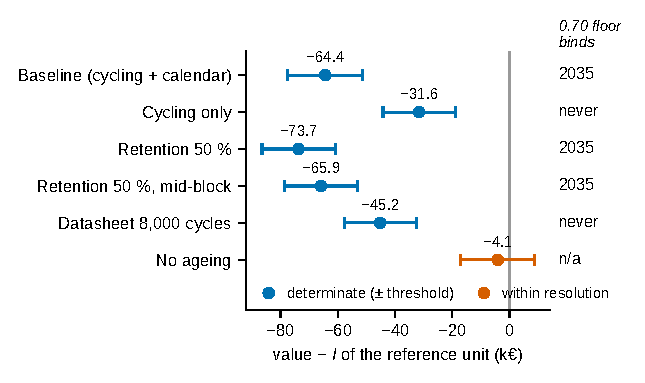
\includegraphics[width=0.90\textwidth]{fig3_ageing_arms_v2.pdf}
    \caption{\textcolor{blue}{Investment margin of the reference unit under alternative ageing calibrations, with the investment plan held fixed. Bars show determinacy thresholds relative to the plan without storage. Right-hand annotations indicate the first year in which the 0.70 state-of-health floor binds; ``never'' indicates that it remains inactive throughout the horizon.}}
    \label{fig:res_ageing}
\end{figure}

\begin{table}[htbp!]
    \centering
    \caption{\textcolor{blue}{Economic and operational performance of the reference unit under alternative ageing calibrations. The investment plan is fixed at 0.25~MVA and 1~MWh, installed at node~7 in 2025.}}
    \label{tab:res_ageing}
    \scriptsize\setlength{\tabcolsep}{3pt}
    \begin{tabular}{l c c c c c c c}
        \toprule
        Calibration & Value (k\euro) & Value $- I$ (k\euro) & Threshold (k\euro) & $\times$ & Binding year & $AE$ & EFC/day \\
        \midrule
        Baseline (cycling + calendar)   & 253.5 & $-$64.4 & 13.1 & 4.93 & 2035  & 0.793 & 0.86 \\
        Cycling only                    & 286.3 & $-$31.6 & 12.6 & 2.50 & never & 0.888 & 1.19 \\
        Retention 50\,\%                & 244.2 & $-$73.7 & 12.8 & 5.74 & 2035  & 0.786 & 0.76 \\
        Retention 50\,\%, mid-block     & 252.1 & $-$65.9 & 12.9 & 5.12 & 2035  & 0.836 & 0.76 \\
        Datasheet 8\,000 cycles         & 272.8 & $-$45.2 & 12.6 & 3.58 & never & 0.834 & 1.13 \\
        No ageing$^{w}$ & 313.8 & $-$4.1 & 12.9 & 0.32 & n/a & 1.000 & 1.29 \\
        \midrule
        Baseline, 0.50 floor & 258.5 & $-$59.5 & 12.6 & 4.71 & never & 0.778 & 1.08 \\
        \bottomrule
    \end{tabular}
    \par\smallskip
    \begin{minipage}{\linewidth}
        \scriptsize
        \raggedright
        \textcolor{blue}{%
            \textit{Note:} Value is the operating-cost reduction relative to the plan without storage under the same calibration; $I=318.0$~k\euro{}. Thresholds follow Subsection~\ref{subsubsec:certification}; $\times$ is the absolute investment margin divided by its threshold. $^{w}$: within resolution; all other margins are determinate. Binding year refers to the 0.70 state-of-health floor, except in the final row, which changes only the floor to 0.50. $AE$ and EFC/day are the present-value-weighted available-energy fraction and equivalent full cycles per day, respectively. ``Never'': the floor remains inactive within the horizon; n/a: not applicable.
    }
    \end{minipage}
\end{table}

\textcolor{blue}{
    The operational results also distinguish the effect of degradation from that of the imposed end-of-life floor. The 0.70 floor first binds in 2035 under the baseline calibration and both variants of the 50\% retention calibration, but remains inactive throughout the horizon under the cycling-only and 8{,}000-cycle datasheet calibrations. Lowering the baseline floor from 0.70 to 0.50 increases cycling by 0.18, 0.20 and 0.27 equivalent full cycles per day in 2025, 2030 and 2035, respectively. Nevertheless, the resulting increase in storage value is only 4.9~k\euro{}, within numerical resolution, and the unit still incurs a determinate shortfall of 59.5~k\euro{}. Thus, relaxing the end-of-life floor permits greater utilisation but does not restore the economic viability of the reference unit under the baseline assumptions. The negative investment margin persists across the tested ageing calibrations, and under the baseline calibration at both floor settings.
}

% --------------------------------------------------------------------------------------------------------------------
\subsection{\textcolor{blue}{Value of Coordination}}
\label{subsec:res_coordination}

\textcolor{blue}{
    Figure~\ref{fig:res_benchmark} and Table~\ref{tab:res_benchmark} compare coordinated operation with the passive and price-taker arrangements defined in Section~\ref{sec:case_settings}. All three arrangements are evaluated without shared storage, thereby separating the benefit of coordination from that of storage investment. The discounted operational cost is 653{,}873.7~k\euro{} under coordination, compared with 744{,}770.3~k\euro{} for the price-taker arrangement and 895{,}049.9~k\euro{} for the passive arrangement. The two static arrangements therefore cost 13.9\% and 36.9\% more than coordinated operation, respectively. The difference relative to the better static arrangement is 90{,}896.6~k\euro{}, approximately 1{,}264 times the larger numerical band of the comparison. All costs are evaluated using the same gross operational cost function, excluding interface settlement.
}

\begin{table}[htbp!]
    \centering
    \caption{\textcolor{blue}{Static no-reverse-flow (NRF) arrangements against coordinated operation at the plan without storage. Each arrangement is the best of three solver starts; in parentheses, the reproducibility band of the coordinated evaluation and the spread of each arrangement over its starts. $\Delta Q$: cost above coordinated operation (k\euro{} and \% of it). Curtailment: day-weighted, over the horizon. Gross operational cost, settlement excluded.}}
    \label{tab:res_benchmark}
    \footnotesize\setlength{\tabcolsep}{3pt}
    \begin{tabular}{l c c c c}
        \toprule
        Arrangement & $Q$ (k\euro) & $\Delta Q$ (k\euro, \%) & TN curt.\ (GWh) & DN curt.\ (GWh) \\
        \midrule
        Coordinated     & 653\,873.7 (71.9) & ---                & ---   & ---   \\
        Price-taker NRF & 744\,770.3 (0.0)  & 90\,896.6 (13.9)   & 807.6 & 0.6   \\
        Passive NRF     & 895\,049.9 (25.8) & 241\,176.2 (36.9)  & 781.7 & 201.2 \\
        \bottomrule
    \end{tabular}
\end{table}

\begin{figure}[htbp!]
    \centering
    \includegraphics[width=1.00\textwidth]{fig5_benchmark.pdf}
    \caption{\textcolor{blue}{Value of coordination at the plan without storage. (a) Gross operational cost $Q$ of the two static no-reverse-flow arrangements (each the best of three solver starts) and of coordinated operation; labels: the difference to coordinated operation. Coordination beats the best static arrangement (price-taker) by 90{,}896.6~k\euro{} (13.9\,\%), 1{,}264 times the larger band (71.9~k\euro). (b) The 90{,}896.6~k\euro{} by agent: the transmission system (77.2\,\%: conventional energy, with 0.81~TWh of transmission renewables left curtailed by the price-taker arrangement) and the distribution systems' flexibility (22.8\,\%). Without any interface rule the transmission network cannot accept the distribution exchange in 1 (passive) and 8 (price-taker) of 12 blocks; coordinated operation uses reverse flow in 4 interface-hours. Settlement excluded.}}
    \label{fig:res_benchmark}
\end{figure}

\textcolor{blue}{
    The decomposition in Fig.~\ref{fig:res_benchmark} attributes 77.2\% of the cost difference between the price-taker and coordinated arrangements to transmission-system operation, through conventional generation costs, and 22.8\% to distribution-system flexibility costs. This result highlights the system-wide consequences of local dispatch decisions. Although the price-taker arrangement limits distribution-level renewable curtailment to 0.6~GWh over the weighted representative periods, transmission-level curtailment remains 807.6~GWh. Exposure to wholesale prices alone therefore does not ensure that distribution flexibility is dispatched consistently with transmission-network conditions. The benefit of coordination is associated with aligning this flexibility with the transmission system's marginal operational value, which reflects its network constraints and operating conditions, rather than with the wholesale price alone.
}

\textcolor{blue}{
    The comparison also depends on the treatment of interface exchanges. Both static arrangements impose a no-reverse-flow rule, whereas coordinated operation determines exchanges jointly and uses reverse flow in four representative interface-hours. When the interface restriction was removed from the static arrangements, the transmission dispatch runs could not accommodate the prescribed distribution exchanges in one of twelve representative year--season blocks for the passive arrangement and eight of twelve for the price-taker arrangement. The reported benefit therefore measures coordination relative to these specific static operating arrangements, including their interface restrictions. It demonstrates substantial operational value at the plan without storage, even though the incremental savings from the storage investments evaluated in Subsection~\ref{subsec:res_baseline} do not recover their investment costs.
}

% --------------------------------------------------------------------------------------------------------------------
\subsection{\textcolor{blue}{Multi-Scenario Instance}}
\label{subsec:res_multiscenario}

\textcolor{blue}{
    The multi-scenario instance combines three market scenarios with three load and renewable-generation scenarios over five representative three-year blocks. 
    The planning search was not repeated at this instance; the reference unit was evaluated against the plan without storage.
    As reported in Table~\ref{tab:res_multiscenario}, the reference unit provides an estimated discounted operational value of 236.7~k\euro{} against an investment cost of 318.0~k\euro{}. The resulting shortfall of 81.3~k\euro{} is 4.52 times the reported resolution of 18.0~k\euro{}, supporting the same economic conclusion as the single-scenario instance. These evaluations were stopped by the production exit of the coordination procedure (ten consecutive cycles passing the residual test with every local solve successful; \ref{app:admm_updated_settings}), rather than by the certification rule of Subsection~\ref{subsubsec:certification}.
}

\textcolor{blue}{
    To assess the sensitivity of the storage-value comparison to this stopping criterion, the evaluation of the plan without storage was continued beyond its stopping point. A subsequent fit to the objective trajectory estimated a further cost decrease of 6.2~k\euro{}. Accounting for this decrease changes the ratio of the reference unit's multi-scenario value to its settled single-scenario value from 0.934 to 0.909. The resulting range therefore reflects the estimated remaining movement of the no-storage evaluation; it is not a certification interval based on $\tau$. The ratio of 0.9331 estimated before the run from the mean-profile price spread lies within this range. Overall, the reference unit's estimated value is approximately 7--9\,\% lower in the multi-scenario instance, while its investment margin remains negative.
    This difference characterises the two evaluated instances and should not be attributed solely to scenario uncertainty, since their temporal discretisation and commitment-cost treatment also differ.
}

\begin{table}[htbp!]
    \centering
    \caption{\textcolor{blue}{The $3 \times 3$ multi-scenario instance: the reference unit (node 7, 0.25~MVA / 1~MWh, 2025) against the plan without storage, and the ratio $R$ of its value to the settled single-scenario value. The multi-scenario evaluations stopped by the production exit; $D$ is the post-hoc settled descent of the $\boldsymbol{x} = \boldsymbol{0}$ evaluation continued past it. Gross operational cost, settlement excluded.}}
    \label{tab:res_multiscenario}
    \scriptsize\setlength{\tabcolsep}{4pt}
    \begin{tabular}{l c l}
        \toprule
        Quantity & Value & Note \\
        \midrule    
        Value $Q(\boldsymbol{0}) - Q(\text{unit})$ at operational stopping (cycle 72 for the plan without storage, 69 for the unit) & 236.7~k\euro & recorded \\
        Investment cost $I$                                                  & 318.0~k\euro & recorded \\
        Value $- I$                                                          & $-$81.3~k\euro & determinate \\
        Resolution of the value                                              & 18.0~k\euro  & $|{\rm value} - I| / {\rm resolution} = 4.52$ \\
        Post-hoc settled descent $D$ of the $\boldsymbol{x} = \boldsymbol{0}$ evaluation & 6.2~k\euro & damped-cosine fit \\
        Settled single-scenario value of the unit                           & 253.5~k\euro & Table~\ref{tab:res_ageing}, baseline \\
        $R$ at operational stopping (upper end)                                     & 0.934 & $V / V^{\text{single}}$ \\
        $R$ after the settled descent (lower end)                            & 0.909 & $(V - D) / V^{\text{single}}$ \\
        $R$ predicted from the mean-profile price spread                     & 0.9331 & recorded before the run \\
        Replay of the $\boldsymbol{x} = \boldsymbol{0}$ evaluation           & 72 / 72 cycles & bitwise \\
        \bottomrule
    \end{tabular}
\end{table}

% --------------------------------------------------------------------------------------------------------------------
\subsection{\textcolor{blue}{Investment Year and Discount Rate}}
\label{subsec:res_sensitivities}

\textcolor{blue}{
    Deferring the reference unit does not make it pay (Table~\ref{tab:res_year_ladder}). Against the plan without storage, the unit installed in 2030 increases the total cost by 68.5~k\euro{} and the unit installed in 2035 by 111.0~k\euro{}. A later installation shortens the part of the horizon over which the unit operates, while the terminal salvage credit returns its remaining calendar life: 11.8~k\euro{} for the 2030 unit and 56.5~k\euro{} for the 2035 unit. The gross difference between the two deferral years, 42.5~k\euro{}, is determinate (3.46 times its threshold of 12.3~k\euro{}); net of salvage it is $-2.3$~k\euro{}, within resolution (0.19 times). In this instance, the choice between deferral years is therefore decided by the salvage convention rather than by operation; net of salvage, the unit costs 54.5--64.4~k\euro{} more than the plan without storage in every investment year. The same holds for two larger plans at node~7: installed in 2030 or 2035, 0.5~MVA / 1~MWh and 0.5~MVA / 2~MWh cost 85.1--223.6~k\euro{} more than the plan without storage, gross or net of salvage, and every difference is determinate (Table~\ref{tab:appE_claims}, rows~17--20).
}

\begin{table}[htbp!]
    \centering
    \caption{\textcolor{blue}{Investment year of the reference unit (node 7, 0.25~MVA / 1~MWh): cost against the plan without storage, $M = I + Q(\boldsymbol{x}) - Q(\boldsymbol{0})$, gross and net of the salvage credit \eqref{eq:salvage_credit}. The 2035 $-$ 2030 difference is determinate gross ($3.46\times$ its threshold of 12.3~k\euro) and within resolution net ($0.19\times$).}}
    \label{tab:res_year_ladder}
    \scriptsize\setlength{\tabcolsep}{5pt}
    \begin{tabular}{l c c c}
        \toprule
        Investment year & $M$ gross (k\euro) & Salvage (k\euro) & $M$ net (k\euro) \\
        \midrule
        2025 (reference) & 64.4  & 0.0  & 64.4 \\
        2030             & 68.5  & 11.8 & 56.7 \\
        2035             & 111.0 & 56.5 & 54.5 \\
        2035 $-$ 2030    & 42.5  & ---  & $-$2.3 \\
        \bottomrule
    \end{tabular}
\end{table}

\textcolor{blue}{
    The conclusion is also robust to the discount rate (Table~\ref{tab:res_discount}). The investment is paid in 2025 and the operational savings accrue over the horizon, so a higher rate lowers the value of the unit, from 277.1~k\euro{} undiscounted to 203.4~k\euro{} at 8\,\%. The unit does not pay at any rate between 0 and 8\,\%: its shortfall grows from 40.8~k\euro{} (2.57 times its threshold) to 114.6~k\euro{} (8.78 times), and every difference is determinate. 
    The rates other than 2\,\% re-weight the per-year costs of the 2\,\% evaluations rather than re-solving them; this is exact at the plan without storage and first-order at the reference unit, whose ageing couples the years.
    Even without discounting, its operational savings over the horizon fall short of its investment cost.
}

\begin{table}[htbp!]
    \centering
    \caption{\textcolor{blue}{Discount rate: the reference unit (node 7, 0.25~MVA / 1~MWh, 2025) against the plan without storage; one discount factor per representative year applied to the five years of its block, $I$ paid in 2025; rates other than 2\,\% re-weight the 2\,\% evaluations; every difference is determinate. Gross operational cost, settlement excluded.}}
    \label{tab:res_discount}
    \scriptsize\setlength{\tabcolsep}{5pt}
    \begin{tabular}{c c c c c c}
        \toprule
        Rate (\%) & Value (k\euro) & $I$ (k\euro) & Value $- I$ (k\euro) & Threshold (k\euro) & $\times$ \\
        \midrule
        0 & 277.1 & 318.0 & $-$40.8  & 15.9 & 2.57 \\
        2 & 253.5 & 318.0 & $-$64.4  & 13.1 & 4.93 \\
        5 & 225.2 & 318.0 & $-$92.7  & 13.1 & 7.10 \\
        8 & 203.4 & 318.0 & $-$114.6 & 13.1 & 8.78 \\
        \bottomrule
    \end{tabular}
\end{table}

\textcolor{blue}{
    Across the 55 comparisons of Table~\ref{tab:appE_claims} reported both gross and net of salvage, applying the salvage credit changes no sign and one verdict: the comparison of the plan returned at twice the base flexibility price with one of its unit neighbours (row~34), which is within the uncertified bar in gross terms (0.95 times) and determinate net of salvage (1.22 times), in the returned plan's favour. The investment-year comparison above is not among them; on it the credit changes both the sign and the verdict, from a determinate 42.5~k\euro{} in gross terms to $-2.3$~k\euro{}, within resolution, net of salvage.
}

% --------------------------------------------------------------------------------------------------------------------
\subsection{\textcolor{blue}{Certification Statistics and Computational Performance}}
\label{subsec:res_certification}

\textcolor{blue}{
    Every certificate used in a reported comparison was decided, or re-decided from its committed record, under the rule of Subsection~\ref{subsubsec:certification}, stated in full in \ref{app:admm_updated_certification}, and certifies at the cycle reported; the single-scenario tables carry these certificates. One earlier certificate, issued under a previous version of the rule and since superseded, is recorded in \ref{app:results} and used in no comparison.
    Of the 42 single-scenario evaluations run under the certification rule of Subsection~\ref{subsubsec:certification} for the comparisons above, 32 certified and 10 did not: 5 were refused by the gap clause, 2 reset by residual lapses and 3 failed by the growth test; each enters its comparison in the uncertified form, with the bar stated beside it. Ten of the 46 certificates the tables use stop within 5\,\% of $\tau$; the rule therefore bounds each evaluation's stopping error at about $\tau$, not well inside it. Evaluations continued past a certificate under this rule moved by at most $0.9\tau$. Passing the residual test alone does not bound this error: on the reference evaluations the objective moved by a further 15--21~k\euro{} after the residual-based stopping rule had certified them, which is why every reported difference carries the threshold of Subsection~\ref{subsubsec:certification} rather than the residual tolerances. Every comparison of this section, and every single-scenario evaluation behind it, is listed in~\ref{app:results}, together with the full certification statistics and the reproducibility record; the search's own evaluations, stopped at the production exit, are reported by their counts, and the multi-scenario pair in Table~\ref{tab:res_multiscenario}.
}

\textcolor{blue}{
    Figure~\ref{fig:res_q_cycle} shows the two outcomes on recorded trajectories. Panel (a) is the settled evaluation of the plan without storage, the reference of every comparison at the base price: certification at cycle 181, 58 cycles after the first residual pass at $k_0 = 123$, with a window range of $0.93\tau$; at cycle 132, where the residual-based rule had stopped this evaluation, the objective still had 15.0~k\euro{} to move. Panels (b) and (c) are the reference unit at 1.5 times the base flexibility price: the objective settles, but the priced interface-consensus gap $t_{\text{sum}}$ stays outside $\pm\tau/2$ to the cap, so the evaluation is reported in the uncertified form (gap 2.5~k\euro, slack 6.3~k\euro{} from the certificate of its earlier run), and its comparison in Table~\ref{tab:res_flex_ladder} is within the bar. The mechanism behind the refused gaps is described in Subsection~\ref{subsec:res_limitations}.
}

\begin{figure}[htbp!]
    \centering
    \includegraphics[width=1.00\textwidth]{fig4_q_versus_cycle.pdf}
    \caption{\textcolor{blue}{Objective against ADMM cycle on two recorded evaluations. (a) The settled evaluation of the plan without storage (single-scenario instance): $Q - Q(k^{*})$ from the first residual pass $k_0 = 123$ to the certification cycle $k^{*} = 181$; circles: the turning points; shaded: the certifying window (the last 32 cycles), whose range (dashed) is $0.93\tau$. $N = 132$: the cycle at which the residual-based rule had stopped this evaluation; $Q$ moved 15.0~k\euro{} after it. (b) The reference unit (node 7, 0.25~MVA / 1~MWh, 2025) at 1.5 times the base flexibility price, refused by the gap clause: $Q - Q(\text{cap})$ from $k_0 = 85$ to the cap at cycle 194; the objective settles, (c) but the priced interface-consensus gap $t_{\text{sum}}$ stays outside $\pm\tau/2$ (ticks: the 59 cycles at which every other clause held and the gap clause refused). Gross operational cost, settlement excluded.}}
    \label{fig:res_q_cycle}
\end{figure}

\textcolor{blue}{
    The three planning searches of Algorithm~\ref{alg:shared_ess_planning_mads} made 41 new recourse evaluations in all (14, 20 and 7 against budgets of 20, 20 and 60), each stopped by the production exit of the coordination procedure and compared at the search resolution $\sigma_Q$ of Section~\ref{sec:case_settings}; the evaluations behind the tables of this section are the re-evaluations of the incumbents, their neighbours and the sensitivity cells under the certification rule, on the final code. 
    Variant A was used for the baseline search and for the first search under the doubled flexibility price, in which every rounded poll direction was inadmissible at every evaluated poll, so that every evaluated point came from the unit-neighbour completion; variant B was used for the certificate of the plan found under that price. Two runs stopped when a unit poll failed and one was stopped for review when its completion set exceeded the cap; the first two are described by their recorded certificates, the third by its stop record and by the certificate of the variant-B run that continued from its incumbent.
    The 42 evaluations run under the rule took 220{,}876~s of wall time over 8{,}570 ADMM cycles, a median of 25.6~s per cycle, one evaluation at a time on a single thread of an Apple M2~Max (\ref{app:results_statistics}). The cost of a planning statement is the cost of its certified evaluations; the search adds the evaluations it proposes and nothing else.
}


% --------------------------------------------------------------------------------------------------------------------
\subsection{\textcolor{blue}{Limitations}}
\label{subsec:res_limitations}

\textcolor{blue}{
    \textbf{Degenerate interface duals.} In some evaluations, storage discharge drives the transmission network's conventional generation to its lower bound while distribution flexibility is at zero activation, where its cost is non-smooth. The interface price $\lambda$, the consensus dual of the interface power, is then set-valued, $\lambda \in [0, c^{\text{flex}}]$, and the consensus converges at the pace of a degenerate dual. This is a known property of the method, not a defect. Certification reports these cases as objective settled, interface-consensus gap unresolved; they appear with large storage and a high flexibility price, and they share one fingerprint, a priced gap of $-8.8$ to $-9.4$~k\euro{} split in the same proportions among the three interface nodes wherever the split was recorded (Table~\ref{tab:appE_gap}). At the base price, the 5~MWh evaluation fails to certify for a different reason: repeated transmission solver recoveries break the growth test, while its consensus gap is small ($+1.1$~k\euro) and of the opposite sign. An economic tie-breaker in the storage agent's objective would remove the degeneracy and is left to future work.
}

\textcolor{blue}{
    \textbf{Solver recoveries and numerical slacks.} In a few transmission blocks some solves reach the iteration limit and recover only to IPOPT's acceptable level; after the first residual pass these number 21 cycles in 10 evaluations, all in transmission blocks, the recurring block being 2035 Spring, and they are excluded from certification evidence (Table~\ref{tab:appE_evaluations}). Renewable output is bounded by availability plus a $10^{-5}$~p.u. numerical slack; the resulting over-production totals about 62~MWh-equivalent over the horizon and is reported separately from the curtailment figures. The monotone branch of the certification rule bounds the remaining descent linearly, without a fit; an evaluation drifting with a half-life longer than its window can certify with drift left beyond $\tau$ (about $3\tau$ is estimated for the reference corner plan's measured half-life at the earlier window of 44 cycles).
}

\textcolor{blue}{
    \textbf{Scope of the study.} The planning search is a heuristic over a lattice with one investment year common to all nodes; per-node timing and staged capacity, which the master problem admits, were not searched, and no optimality certificate is claimed: the result is that no evaluated plan pays at the baseline, with every evaluated unit neighbour of the plan without storage worse, determinately for the eight re-evaluated under the certification rule (Table~\ref{tab:appE_neighbours}) and beyond the search resolution for the other six. The ageing arms re-evaluate a fixed plan rather than re-optimising it; since the reference unit loses determinately under every aged arm and the value is affine in size on the evaluated ladders, the plan without storage is the search's answer under each of them, but this was not run. The horizon is three representative years each standing for a five-year block (five three-year blocks at the multi-scenario instance), with four representative days per year; the discretization is a modelling choice and the degradation chain is applied at block boundaries. 
    The multi-scenario evidence is the $3 \times 3$ instance: the $5 \times 5$ scenario set of the submitted version could not be evaluated within the memory available and is left to future work. The certification bounds the stopping error of each evaluation, not the local solution that the nonconvex coordination reaches: a different penalty schedule or starting point could reach a different local solution; where this was measured, for the static arrangements of Subsection~\ref{subsec:res_coordination}, the spread over three solver starts is reported (Table~\ref{tab:res_benchmark}).
    The test system (one 9-bus transmission network with three 33-bus distribution networks) limits the generality of the conclusions. The salvage credit is reported, not optimized, and the attribution of degradation to the transmission and distribution operators is not unique under a jointly determined schedule and is not attempted. Finally, the 0.70 state-of-health floor raises the elasticity of value to available energy ($\varepsilon_{AE}$ 1.04--1.85, against 0.41--0.62 for the same three resolvable arms at a 0.50 floor); this is read as a late-life tail effect, the floor removing the low-SoH years whose throughput is least valuable, but the decomposition that would show it has not been measured.
}

% ====================================================================================================================
%                                                      CONCLUSIONS                                                    
% ====================================================================================================================
\section{Conclusions}
\label{sec:conclusions}

\textcolor{blue}{
    This paper presented a degradation-aware framework for planning shared ESSs at TN--DN interface nodes. Planning is formulated as a two-stage stochastic program whose first stage selects a single, discrete investment plan and whose recourse is the coordinated TSO--DSO operation of that plan, a nonconvex problem with AC network models and the ageing of the storage over the horizon. Candidate plans are proposed by a derivative-free search over the lattice of commercial unit sizes and evaluated by consensus-ADMM coordination with a dedicated shared-ESS agent. Because the recourse is nonconvex, the method claims no optimality certificate; instead, each evaluation behind a reported comparison has a stated stopping status --- certified by an explicit rule, uncertified with its error bar, or, at the multi-scenario instance, stopped by the production exit, with the remaining movement of the plan without storage estimated from a continued run --- and every planning comparison is reported with the resolution at which it is decided, the search's own evaluations at the search resolution.
}

\textcolor{blue}{
    On an integrated 108-bus system, the search returned no investment at the baseline: the reference unit (0.25~MVA / 1~MWh) falls 64.4~k\euro{} short of its investment cost of 318.0~k\euro{}, and every other plan of Table~\ref{tab:res_value_ladder}, from 0.5 to 5~MWh and at one or two nodes, also loses determinately. Degradation decides this result. Without ageing the reference unit is at break-even, within resolution; with ageing it loses 31.6--73.7~k\euro{} across the calibrations tested, and lowering the end-of-life floor from 0.70 to 0.50 does not change the verdict. For 4~h storage at node~7 the break-even energy cost is 171--193~k\euro/MWh, against 254~k\euro/MWh at the baseline, and the reference unit pays at 1.75 and 2 times the base flexibility price; at 2 times, the search returns a two-node plan. The verdict at the baseline holds for discount rates of 0--8\,\%, for deferral of the investment to 2030 or 2035, and on the multi-scenario instance, where the storage value is 7--9\,\% lower. Coordination itself is worth 13.9\,\% of the operating cost, 90.9~M\euro{}, against the best static no-reverse-flow arrangement at the plan without storage, through the dispatch of distribution flexibility against the transmission network's marginal value rather than the wholesale price.
}

\textcolor{blue}{
    Two implications follow. For planning, ageing decides the value of shared storage on this system, the same unit being at break-even without it and losing with it; and the coordinated operation that would give storage its value is itself the larger benefit, while storage becomes worthwhile where flexibility is expensive. 
    For the method, a residual-based stopping test is not sufficient on a nonconvex recourse: on the reference evaluations the objective moved by a further 15--21~k\euro{} after that test had been passed, the same order as the planning differences reported on an operating cost of 654~M\euro{}; stating the resolution of every evaluation is what makes such differences interpretable.
}

\textcolor{blue}{
    The search explored plans with one investment year common to all nodes. Per-node timing and staged expansion, which the master problem admits, larger test systems, and an economic tie-breaker for the degenerate interface prices that left some evaluations at high flexibility prices uncertified are the next steps.
    Future work will also extend the framework to other shared flexibility resources, to richer representations of degradation and uncertainty, and to an allocation of the degradation of a shared asset among the operators that use it.
}

\appendix

% ====================================================================================================================
%                                                        APPENDIX                                                     
% ====================================================================================================================

\section{\textcolor{blue}{TSO--DSO Coordinated Operational Planning}}
\label{app:admm_updated}

\textcolor{blue}{
    This appendix states the coordination procedure that evaluates a candidate plan, as implemented: the consensus ADMM of~\cite{simoes_2023} extended with the shared-ESS agent of Subsection~\ref{subsec:subproblem}. It is a three-agent, global-variable consensus on the storage schedule, combined with a pairwise consensus on each TN--DN interface, run as a sweep (DSOs, then TSO, then the storage agent) that is Gauss--Seidel on the interface channels and, on the storage channel, a global-variable consensus in which all three agents solve against the same $z$ before it is updated; the penalty parameters follow residual balancing, and the iteration uses Anderson acceleration and a tightened interior-point tail.
    The stopping test is stated here; the certification rule that decides when an evaluation's value may be used is Subsection~\ref{subsubsec:certification}.
}

\subsection{\textcolor{blue}{Agents, Blocks and Consensus Variables}}
\label{app:admm_updated_agents}

\textcolor{blue}{
    A \emph{block} is one representative year $y$ and one representative day $d$. The TSO holds one network model per block; each DSO $i \in N^I$ holds one model of its DN per block; every scenario of the block lives inside the same model, with the objective weighted by the scenario probabilities. The shared-ESS agent holds one model per interface node $e \in E^S$ spanning all years, days and hours, and no scenario index. Each network block objective is divided by a common scale $\sigma$ and multiplied by its block weight $w_{y,d} = Y_y D_d (1+r)^{-(y-y_0)}$, so that every block is solved in the same units and the sum over blocks, after the exclusions of Subsection~\ref{subsubsec:certification}, is the discounted operating cost of \eqref{eq:recourse_value}.
}

\textcolor{blue}{
    Three families of consensus variables couple the agents. On the interface of DN $i$: the voltage $V^{\text{I}}_{i,y,d,t}$ and the active and reactive power exchanges $P^{\text{I}}_{i,y,d,t}$, $Q^{\text{I}}_{i,y,d,t}$, shared by the TSO and DSO~$i$; in the multi-scenario instance these are the \emph{expected} interface quantities, $\sum_{s \in \Omega_M \times \Omega_O} \omega_s P^{\text{I}}_{i,s,t}$, of Subsection~\ref{subsubsec:commitment}. On each shared ESS: the active and reactive power $P^{\text{E}}_{e,y,d,t}$, $Q^{\text{E}}_{e,y,d,t}$, shared by the TSO, the DSO of node $e$ and the storage agent through a global variable $z_{e,y,d,t} = (z^{P}, z^{Q})$. Each agent $a$ keeps its own copy $x_a$ of every consensus variable it shares and a dual variable $\lambda_a$ for it; the storage channel carries one copy and one dual per agent (three of each), the interface channels one per side.
}

\textcolor{blue}{
    Consensus terms are written on normalised differences: the interface powers are divided by the rating $R^{\text{I}}_i$ of the DN's interface transformer, the storage powers by $2 S^{\text{ref}}$ with $S^{\text{ref}}$ a reference converter rating common to all nodes, years and candidates, and the interface voltage is left in per unit.
    The storage agent's augmented-Lagrangian terms are multiplied by $\kappa^{\text{E}} = \sigma / \operatorname{median}_b w_b$, which is equivalent to dividing the agent's local objective by $\kappa^{\text{E}}$ and puts it on the same footing as a median block's scaled objective.
}

\subsection{\textcolor{blue}{Local Problems}}
\label{app:admm_updated_implementation}

\textcolor{blue}{At cycle $k$ the TSO and each DSO solve their block models with the consensus terms added to the
scaled local objective. For a network agent $a$ with local objective $f_a$ and interface counterpart $\hat{x}$ (the
other side's current copy), the problem of block $(y,d)$ is}

\textcolor{blue}{
    \begin{equation}
        \begin{aligned}
            \min_{x_a} \;
            & \frac{w_{y,d}}{\sigma} f_a(x_a)
            + \sum_{i} \sum_{t} \Big[
                \lambda^{V}_{a,i,t} \big(V^{\text{I}}_{a,i,t} - \hat{V}^{\text{I}}_{i,t}\big)
                + \frac{\rho^{V}}{2} \big(V^{\text{I}}_{a,i,t} - \hat{V}^{\text{I}}_{i,t}\big)^2
              \Big] \\
            & + \sum_{i} \sum_{t} \sum_{\xi \in \{P,Q\}} \Big[
                \lambda^{\xi}_{a,i,t} \frac{\xi^{\text{I}}_{a,i,t} - \hat{\xi}^{\text{I}}_{i,t}}{R^{\text{I}}_i}
                + \frac{\rho^{\text{PF}}}{2} \Big( \frac{\xi^{\text{I}}_{a,i,t} - \hat{\xi}^{\text{I}}_{i,t}}{R^{\text{I}}_i} \Big)^2
              \Big] \\
            & + \sum_{e} \sum_{t} \sum_{\xi \in \{P,Q\}} \Big[
                \lambda^{\xi}_{a,e,t} \frac{\xi^{\text{E}}_{a,e,t} - z^{\xi}_{e,t}}{2 S^{\text{ref}}}
                + \frac{\rho^{\text{E}}}{2} \Big( \frac{\xi^{\text{E}}_{a,e,t} - z^{\xi}_{e,t}}{2 S^{\text{ref}}} \Big)^2
              \Big]
        \end{aligned}
        \label{eq:admm_network_local}
    \end{equation}
}

\noindent
\textcolor{blue}{subject to the agent's network constraints, the storage model of
Subsection~\ref{subsubsec:network_storage} with the available capacities received from the storage agent, and, in the
multi-scenario instance, the commitment terms of Subsection~\ref{subsubsec:commitment}. The block index $(y,d)$ is
omitted from the variables; the interface sums run over the DNs the agent is connected to (one, for a DSO), and the
storage sums over the shared ESSs at its nodes. The storage agent solves, over all blocks at once,}

\textcolor{blue}{
    \begin{equation}
        \begin{aligned}
            \min_{x_{\text{E}}} \;
            & f_{\text{E}}(x_{\text{E}})
            + \kappa^{\text{E}} \sum_{e} \sum_{y,d,t} \sum_{\xi \in \{P,Q\}} \Big[
                \lambda^{\xi}_{\text{E},e,y,d,t} \frac{\xi^{\text{Net}}_{e,y,d,t} - z^{\xi}_{e,y,d,t}}{2 S^{\text{ref}}} \\
            & \qquad\qquad
                + \frac{\rho^{\text{E}}}{2} \Big( \frac{\xi^{\text{Net}}_{e,y,d,t} - z^{\xi}_{e,y,d,t}}{2 S^{\text{ref}}} \Big)^2
              \Big]
        \end{aligned}
        \label{eq:admm_esso_local}
    \end{equation}
}

\noindent
\textcolor{blue}{
    subject to \eqref{eq:cohort_rated}--\eqref{eq:available_capacity}, \eqref{eq:esso_net_power}--\eqref{eq:soh_floor}, the bounds $0 \le P^{\text{Ch}}, P^{\text{Dch}} \le S^{\text{Rated,Unit}}$ on each cohort's powers and the converter capability inequality $(P^{\text{Net}}_{e,y,d,t})^2 + (Q^{\text{Net}}_{e,y,d,t})^2 \le (S^{\text{Av}}_{e,y})^2$ on its aggregate schedule, where $f_{\text{E}}$ is the agent's local objective,
}

\textcolor{blue}{
    \begin{equation}
        \begin{aligned}
            f_{\text{E}}(x_{\text{E}}) = \;
            & c^{\sigma} \sum_{e \in E^S} \sum_{y \in Y} \sum_{d \in D} \sum_{t \in T}
            \left( \sigma^{+}_{e,y,d,t} + \sigma^{-}_{e,y,d,t} \right)\\
            & + \varepsilon^{\text{E}} \sum_{e \in E^S} \sum_{y^\text{Inv} \in Y} \sum_{y \in Y} \sum_{d \in D} \sum_{t \in T}
            \left( P^{\text{Ch}}_{e,y^\text{Inv},y,d,t} + P^{\text{Dch}}_{e,y^\text{Inv},y,d,t} \right)
        \end{aligned}
        \label{eq:esso_objective}
    \end{equation}
}

\noindent
\textcolor{blue}{
    a feasibility penalty on the slack pair of \eqref{eq:esso_net_power} and a linear regularization of throughput. The weight $\varepsilon^{\text{E}}$ is far below the resolution of Subsection~\ref{subsubsec:certification} and serves one purpose: with a linear, strictly positive price on $P^{\text{Ch}} + P^{\text{Dch}}$, simultaneous charging and discharging is never optimal, so complementarity in the agent follows from the problem structure and needs no nonconvex constraint; the residual $\min\{P^{\text{Ch}}, P^{\text{Dch}}\}$ is checked after every solve and recorded, not enforced, and at the certified points it was below $4 \times 10^{-5}$ of the rating. The values of $c^{\sigma}$ and $\varepsilon^{\text{E}}$ are given in Section~\ref{sec:case_ess_params}.
    The penalty parameters $\rho^{V}$, $\rho^{\text{PF}}$ and $\rho^{\text{E}}$ are one per channel, common to all agents and to active and reactive power. A proximal term on the TSO's consensus variables is implemented but was run with weight zero.
}

\subsection{\textcolor{blue}{Consensus, Dual and Penalty Updates}}
\label{app:admm_updated_updates}

\textcolor{blue}{
    After the storage agent has solved, the global storage variable is updated as the weighted average of the three copies, with weights $\rho^{\text{E}} \alpha^2$ and the duals folded in, and every agent's dual is updated against it ($\alpha = 1/(2 S^{\text{ref}})$, $\xi \in \{P,Q\}$, $a \in \{\text{TSO}, \text{DSO}_i, \text{E}\}$):
}

\textcolor{blue}{
    \begin{equation}
        \begin{aligned}
            z^{\xi,k+1}_{e,y,d,t} &=
            \frac{\sum_{a} \big( \rho^{\text{E}} \alpha^2\, \xi^{k+1}_{a,e,y,d,t} + \alpha\, \lambda^{\xi,k}_{a,e,y,d,t} \big)}
                 {\sum_{a} \rho^{\text{E}} \alpha^2}, \\
            \lambda^{\xi,k+1}_{a,e,y,d,t} &= \lambda^{\xi,k}_{a,e,y,d,t} + \rho^{\text{E}} \alpha
            \big( \xi^{k+1}_{a,e,y,d,t} - z^{\xi,k+1}_{e,y,d,t} \big)
        \end{aligned}
        \label{eq:admm_z_update}
    \end{equation}
}

\noindent
\textcolor{blue}{
    which is the minimiser over $z$ of the three agents' consensus terms taken with unit weight; the factor $\kappa^{\text{E}}$ scales the storage agent's local problem only and does not enter the update. The interface duals of both sides are updated after the TSO's solve, each against the other side's copy ($\xi \in \{P,Q\}$):
}

\textcolor{blue}{
    \begin{equation}
        \lambda^{V,k+1}_{a,i,t} = \lambda^{V,k}_{a,i,t} + \rho^{V} \big( V^{\text{I},k+1}_{a,i,t} - V^{\text{I},k+1}_{\bar a,i,t} \big),
        \qquad
        \lambda^{\xi,k+1}_{a,i,t} = \lambda^{\xi,k}_{a,i,t} + \rho^{\text{PF}}\,
        \frac{\xi^{\text{I},k+1}_{a,i,t} - \xi^{\text{I},k+1}_{\bar a,i,t}}{R^{\text{I}}_i}
        \label{eq:admm_interface_duals}
    \end{equation}
}

\noindent
\textcolor{blue}{
    where $\bar a$ is the counterpart of $a$ on interface $i$. An agent whose solve failed keeps its previous copy; the interface duals of a block are updated only when both its TSO and its DSO solves succeeded, and $z$ and the three storage duals of a node only when all three solves succeeded.
}

\textcolor{blue}{
    The penalty parameters follow residual balancing~\cite{boyd_admm_2011}, per channel $g \in \{V, \text{PF}, \text{E}\}$ and with one value for all agents: with $r_g$ and $s_g$ the primal and dual residuals of the channel and $\varepsilon^{\text{pri}}_g$, $\varepsilon^{\text{dual}}_g$ their tolerances (\ref{app:admm_updated_stopping}), $\rho_g \gets 1.5\,\rho_g$ when $r_g/\varepsilon^{\text{pri}}_g > \mu\, s_g/\varepsilon^{\text{dual}}_g$ and $\rho_g \gets \rho_g/1.5$ when $s_g/\varepsilon^{\text{dual}}_g > \mu'\, r_g/\varepsilon^{\text{pri}}_g$, with $\mu = 5$ and $\mu' = 5$ ($\mu' = 3$ for the decrease of $\rho^{\text{PF}}$), clamped to $[10^{-4}, 10^{4}]$. The storage channel is exempt from balancing until its dual ratio has been below one on five consecutive cycles (its two-phase schedule), a channel freezes once it has gone ten cycles without changing after having acted, every channel freezes at cycle 200, and a cycle with a failed solve leaves every $\rho_g$ unchanged. Any change of a $\rho_g$ clears the acceleration memory. In the certifying regime of Subsection~\ref{subsubsec:certification} all $\rho_g$ are frozen from the cycle after the first residual pass $k_0$, or, in the three reference evaluations continued from an earlier run, from the cycle after that run's stopping cycle.
}

\subsection{\textcolor{blue}{Stopping Test, Acceleration and Tail}}
\label{app:admm_updated_stopping}

\textcolor{blue}{
    Convergence is tested once per cycle, after the storage agent. For the storage channel the primal residual is $r_{\text{E}} = \lVert \alpha (x - z) \rVert$ over all agents, nodes and hours and the dual residual $s_{\text{E}} = \lVert \rho^{\text{E}} \alpha\, \Delta z \rVert$ taken over the three agents (so $\sqrt{3}\,\rho^{\text{E}} \alpha \lVert \Delta z \rVert$); for the interface channels $r = \lVert (x_{\text{DSO}} - x_{\text{TSO}}) / b \rVert$ and $s = \rho \lVert \Delta x_{\text{TSO}} / b \rVert$ with $b$ the channel's normalisation ($R^{\text{I}}_i$ for the powers, one for the voltage). The tolerances are those of Boyd et al.~\cite{boyd_admm_2011}, $\varepsilon^{\text{pri}} = \sqrt{n}\,\varepsilon_{\text{abs}} + \varepsilon_{\text{rel}} \max\{\lVert x \rVert, \lVert z \rVert\}$ and $\varepsilon^{\text{dual}} = \sqrt{n}\,\varepsilon_{\text{abs}} + \varepsilon_{\text{rel}} \lVert \lambda \rVert$, with $\lambda$ the DSO-side dual on the interface channels and all three duals on the storage channel, with $n$ the channel's dimension and $\varepsilon_{\text{abs}} = 10^{-5}$, $\varepsilon_{\text{rel}} = 10^{-4}$. A cycle passes when every channel is within its tolerances and every local solve of the cycle ended at a status the solver reports as solved (optimal or acceptable). 
    The production exit is ten consecutive passing cycles; it stopped the multi-scenario evaluations. The single-scenario evaluations of this paper were stopped by the certification rule of Subsection~\ref{subsubsec:certification} or by its cycle cap, whichever came first; the holds start at the first passing cycle, while the rule's own $k_0$ resets on a lapse. Objective-change tests are computed for diagnosis only.
}

\textcolor{blue}{
    Between cycles a type-II Anderson acceleration~\cite{walker_ni_2011} is applied, on the storage channel, to $z$ and the three agents' $\lambda_a/\rho$ and, on each interface channel, to the TSO's copy and the DSO-side $\lambda/\rho$, with memory 5 and a Tikhonov regularisation of $10^{-10}$. The accelerated point is accepted only if the combined residual $\sqrt{\sum_g (r_g^2 + s_g^2)}$ is below its value at the last accepted step; on rejection the memory is kept. 
    The memory is cleared on any change of a penalty parameter and on any failed local solve, and the acceleration is switched off on any cycle in which every channel passes and, in the certifying regime, from the cycle after $k_0$ on (or after the earlier run's stopping cycle in a continued evaluation).
}

\textcolor{blue}{
    In the cycle after a cycle in which every channel passed and every solve succeeded, the TSO and DSO solves are run with the interior-point complementarity tolerance tightened to $10^{-6}$ (the tight tail); the production setting restores each operator's own tolerance otherwise (the tail is a declared option, enabled in every campaign behind the reported tables), and the certifying regime holds the tail on from the cycle after $k_0$. A local solve that ends at the iteration limit, infeasible or in a solver error is retried in two tiers, a cold restart with the agent's recovery settings and the same with the adaptive barrier strategy (\ref{app:admm_updated_settings}); an exit at the solver's acceptable level is counted as a successful solve for the stopping test, and the certification rule decides separately whether the cycle is clean.
}

\subsection{\textcolor{blue}{Certification Rule}}
\label{app:admm_updated_certification}

\textcolor{blue}{
    The certifying regime of Subsection~\ref{subsubsec:certification} opens at the residual pass $k_0$. Throughout the regime acceleration is off, the tight interior-point tail is on and the penalty parameters $\rho$ are frozen, from the cycle after $k_0$, or, in the three reference evaluations continued from an earlier run, from the cycle after that run's stopping cycle (an evaluation re-run on an earlier record replays it bitwise to its first residual pass and holds from the cycle after it);
    a later lapse of the residual test, or a cycle with a failed solve, resets $k_0$ and the turning-point record while these holds stay. With $Q_k$ the value of the recourse objective at cycle $k$, the evaluation is certified on the oscillatory branch at the first cycle $k^{\star} > k_0$ at which:
}

\textcolor{blue}{
    \begin{enumerate}
        \item[(C1)] \emph{Period}: $Q_k$ has shown at least three turning points since $k_0$, and its period $\hat{P}$, the number of cycles spanned by the three most recent, is measured rather than assumed;
        \item[(C2)] \emph{Damping} (the growth test): its successive half-swings are not growing;
        \item[(C3)] \emph{Settling}: with $n_{\mathrm{w}}$ denoting the certifying-window length in ADMM cycles, its range over the last $n_{\mathrm{w}} = \max\{20, \lceil 1.1\,\hat{P} \rceil\}$ cycles, all after $k_0$, is at most $\tau$;
        \item[(C4)] \emph{Consensus} (the gap clause): the priced interface-consensus gap $t_{\text{sum}}$, the value of the residual mismatch between the operators' interface active-power schedules at the expected wholesale price of each hour, block-weighted, satisfies $|t_{\text{sum}}| \le \tau/2$;
        \item[(C5)] \emph{Clean evidence}: every cycle in that window was solved cleanly, every local solve ending at the solver's optimal status, or at its acceptable status on a primary attempt with all four termination metrics within ten times the tight-tail tolerances.
    \end{enumerate}
}

\textcolor{blue}{
    In (C1)--(C2) a step smaller than $\tau/100$ carries no sign, a swing smaller than $\tau/10$ is treated as noise and is neither compared nor counted as a turning point, and the first three cycles after $k_0$ are not counted. An objective that descends without a sign change is certified instead on the monotone branch, over a window of $2P_{\max}$ cycles after $k_0$ with $P_{\max}$ the longest period measured on the instance, when (M1) its steps are decreasing --- the mean step over the second half of the window is below that over the first half, or every step is below $\tau/100$; (M2) its range is at most $\tau$; (M3) $|\text{last step}| \cdot 2P_{\max} \le \tau$, a linear bound on the remaining descent that uses no fit; and (C4)--(C5) hold on that window. An evaluation that satisfies neither branch within its cycle cap is reported in the uncertified form of Subsection~\ref{subsubsec:certification}: its consensus gap is $|t_{\text{sum}}|$ at the cap, and its settling slack is the movement of the objective between the certification cycle of its earlier, residual-based run and the cap.
}

\subsection{\textcolor{blue}{Algorithm}}
\label{app:admm_updated_algorithm}

\textcolor{blue}{
    Algorithm~\ref{alg:operational_planning_degradation} summarises one recourse evaluation. The storage agent publishes the available capacities $S^{\text{Av}}_{e,y}$ and $E^{\text{Av}}_{e,y}$ of \eqref{eq:available_capacity} to every network block before each cycle, so that the degraded capacities bound the state of charge and the converter in the operators' models; after the initialisation solves, the plan $\boldsymbol{x}$ enters a network model only through these capacities.
}

\begin{algorithm}[htbp!]
    \caption{\textcolor{blue}{Consensus ADMM evaluation of a candidate plan with the shared-ESS agent}}
    \label{alg:operational_planning_degradation}
    \DontPrintSemicolon

    \KwIn{Plan $\boldsymbol{x}$; network and market data of every block; ESS parameters; $\rho^{V}_0$, $\rho^{\text{PF}}_0$, $\rho^{\text{E}}_0$; $\varepsilon_{\text{abs}}$, $\varepsilon_{\text{rel}}$; cycle cap $k^{\max}$; certification parameters of \ref{app:admm_updated_certification}.}
    \KwOut{$Q(\boldsymbol{x})$ with its certification record, or the uncertified form.}

    \tcp{Initialisation}
    \ForEach{DSO $i \in N^I$ and block $(y,d)$}{
        Build the DN model with the plan's storage at its interface node; solve it standalone with the interface voltage at its nominal value; record its expected interface exchange\;
    }
    \ForEach{block $(y,d)$}{
        Build the TN model with each DN represented by its recorded expected exchange; solve it standalone\;
    }
    Build the storage agent's model from $\boldsymbol{x}$; solve it standalone with its powers fixed at the TSO's initial
    storage schedule\;
    Convert every model to its ADMM form \eqref{eq:admm_network_local}, \eqref{eq:admm_esso_local} with $\rho_g \gets \rho_{g,0}$ (the interface settlement's weight is set to one here and, in the multi-scenario instance, the commitment charge is activated); 
    $z \gets$ the average of the three agents' storage copies; storage duals at zero; interface duals set by one dual-ascent step from zero on the initial solutions; $k \gets 1$\;

    \tcp{Cycles}
    \While{$k \le k^{\max}$}{
        Publish $S^{\text{Av}}_{e,y}$, $E^{\text{Av}}_{e,y}$ from the storage agent to every network block\;
        \ForEach{DSO $i$ and block $(y,d)$}{
            Set $\hat{V}^{\text{I}}, \hat{P}^{\text{I}}, \hat{Q}^{\text{I}}$ to the TSO's current copies and the storage
            target to $z$; solve \eqref{eq:admm_network_local}\;
        }
        \ForEach{block $(y,d)$}{
            TSO: set $\hat{V}^{\text{I}}, \hat{P}^{\text{I}}, \hat{Q}^{\text{I}}$ to the DSOs' new copies and the storage
            target to $z$; solve \eqref{eq:admm_network_local}\;
        }
        Update the interface duals of both sides, \eqref{eq:admm_interface_duals}\;
        Storage agent: set the target to $z$; solve \eqref{eq:admm_esso_local}; update the SoH chain and the available capacities\;
        Update $z$ and the three storage duals, \eqref{eq:admm_z_update}, for every block and node whose solves all succeeded\;
        Evaluate the residual test of \ref{app:admm_updated_stopping}; record the objective, residuals and solve statuses of the cycle (the priced interface gap is recorded by the campaign harness)\;
        Apply the Anderson step (unless off); balance $\rho_g$ (unless frozen) and clear the acceleration memory if
        any $\rho_g$ changed; set the tight tail for the next cycle\;
        \If{the stopping rule in force is met (production: ten consecutive passing cycles; single-scenario tables: the certification rule, with its holds)}{
            \textbf{exit}\;
        }
        $k \gets k + 1$\;
    }
    \Return{the objective and record of the certification cycle, or the uncertified form}\;
\end{algorithm}

\subsection{\textcolor{blue}{Scenario Mechanics of the Multi-Scenario Instance}}
\label{app:admm_updated_scenarios}

\textcolor{blue}{
    When several market and operation scenarios are present in a block, the interface consensus is on the expected exchange, the TSO represents each DN by the DN's expected exchange at initialisation, held fixed, plus a scenario-free adjustment bounded by the interface rating as its only interface freedom (the same construction at one scenario), and the storage schedule is one scenario-free variable (Subsections~\ref{subsubsec:network_storage} and~\ref{subsubsec:commitment}). The commitment-deviation charge is inactive in the initialisation solves and is activated with the interface settlement when the models are converted to their ADMM form. The interface settlement is carried at full weight: its contracted part is removed from the reported cost as a transfer, its deviation part is kept. A quadratic regularisation of the interface-voltage dispersion across scenarios is added to the TSO and DSO models as a solver-side term and removed from the reported cost. At a single scenario the commitment charge and the voltage regularisation are not constructed; the interface settlement remains in every local objective at full weight and is excluded from the reported cost as a transfer.
}

\subsection{\textcolor{blue}{Solver and Coordination Settings}}
\label{app:admm_updated_settings}

\textcolor{blue}{
    The frozen configuration of Section~\ref{sec:case_settings} is as follows.
    Local problems were solved with IPOPT~3.14.18 through Pyomo~6.9.5 on Python~3.11.11, the network models with the MA97 linear solver and the storage agent with MA57, single-threaded throughout. Network solves use a convergence tolerance of $10^{-5}$, an acceptable tolerance of $10^{-4}$, a complementarity tolerance of $5 \times 10^{-4}$ (TSO) and $10^{-4}$ (DSOs), and at most 500 iterations; the tight tail sets the complementarity tolerance to $10^{-6}$. The storage agent solves to a tolerance of $10^{-10}$ with an acceptable tolerance of $10^{-9}$. A solve that ends at the iteration limit, infeasible or in a solver error is retried as a cold restart with the agent's recovery settings (TSO: acceptable tolerance $10^{-4}$ after one acceptable iteration; DSOs: their primary settings; storage agent: acceptable tolerance $10^{-9}$ after one iteration) and then once more with the adaptive barrier strategy.
}

\textcolor{blue}{
    The ADMM settings are: common objective scale $\sigma = 93{,}635{,}360$; reference converter rating $S^{\text{ref}} = 2.5$~MVA; interface-transformer ratings $R^{\text{I}} = 2.0$, $1.0$ and $1.5$~p.u. (200, 100 and 150~MVA on a 100~MVA base) at TN nodes 5, 7 and 9; storage-agent scale $\kappa^{\text{E}} = \sigma/\operatorname{median}_b w_b$ ($227{,}211$ at the single-scenario instance, $386{,}259$ at the multi-scenario instance); initial penalties $\rho^{V}_0 = 0.0077$, $\rho^{\text{PF}}_0 = 0.198$, $\rho^{\text{E}}_0 = 0.01$; residual balancing with ratio 5 (3 for the decrease of $\rho^{\text{PF}}$), factor 1.5, bounds $[10^{-4}, 10^{4}]$, a per-channel freeze after ten unchanged cycles and a backstop at cycle 200, the storage channel exempt until its dual ratio has been below one on five consecutive cycles; residual tolerances $\varepsilon_{\text{abs}} = 10^{-5}$, $\varepsilon_{\text{rel}} = 10^{-4}$; Anderson acceleration with memory 5 and regularisation $10^{-10}$. The production exit is ten consecutive passing cycles, with a cap of 500 cycles at the multi-scenario instance. 
    In the multi-scenario instance the solver-side voltage regularisation weight is $9 \times 10^{4}$.
}

\section{Market Data}
\label{app:market_data}

This appendix presents the seasonal wholesale energy and flexibility market price profiles used in the case study. All price trajectories correspond to the base year (2025); annual growth assumptions are given in Section~\ref{sec:case_studies}. 
Figure~\ref{fig:cs3_market_prices} shows the profiles adopted for the summer, autumn, and winter representative days of 2025, respectively. 

\begin{figure*}[htbp]
    \centering
    \subfloat[Spring 2025]{
        \includegraphics[width=0.475\textwidth]{SRP1_market_prices_2025_Spring.pdf}
    }
    \hfill
    \subfloat[Summer 2025]{
        \includegraphics[width=0.475\textwidth]{SRP1_market_prices_2025_Summer.pdf}
    }
    \\[5pt]
    \subfloat[Autumn 2025]{
        \includegraphics[width=0.475\textwidth]{SRP1_market_prices_2025_Autumn.pdf}
    }
    \hfill
    \subfloat[Winter 2025]{
        \includegraphics[width=0.475\textwidth]{SRP1_market_prices_2025_Winter.pdf}
    }
    \caption{Wholesale energy and flexibility market prices in 2025.}
    \label{fig:cs3_market_prices}
\end{figure*}

\section{Transmission Network}
\label{app:tn_description}

This appendix presents the RES generation scenarios adopted for the TN in the base planning year (2025). The profiles reflect seasonal variability in wind and solar production and are used as baseline trajectories in all representative years, scaled according to the installed-capacity evolution described in Section~\ref{sec:case_studies}. Figure~\ref{fig:cs3_tn_res_scenarios_2025} shows the RES generation profiles adopted for the spring, summer, autumn, and winter representative days of 2025, respectively.

\begin{figure*}[htbp]
    \centering
    \subfloat[Spring 2025]{
        \includegraphics[width=0.475\textwidth]{case9_RES_generation_scenarios_2025_Spring.pdf}
    }
    \hfill
    \subfloat[Summer 2025]{
        \includegraphics[width=0.475\textwidth]{case9_RES_generation_scenarios_2025_Summer.pdf}
    }
    \\[5pt]
    \subfloat[Autumn 2025]{
        \includegraphics[width=0.475\textwidth]{case9_RES_generation_scenarios_2025_Autumn.pdf}
    }
    \hfill
    \subfloat[Winter 2025]{
        \includegraphics[width=0.475\textwidth]{case9_RES_generation_scenarios_2025_Winter.pdf}
    }
    \caption{TN RES generation profiles for the seasonal scenarios in 2025.}
    \label{fig:cs3_tn_res_scenarios_2025}
\end{figure*}

\section{Distribution Networks}
\label{app:dns_description}

This appendix presents the seasonal RES generation, load, and flexibility profiles adopted for the three ADNs connected to the TN. Although all ADNs share the IEEE 33-bus topology, they differ in installed RES capacities and flexibility penetration, resulting in heterogeneous operating conditions across TN--DN interfaces.
Tables~\ref{tab:cs1_ieee33_buses}--\ref{tab:cs1_ieee33_loads} report the bus, branch, TN connection, and load data common to all ADNs in the case study of Section~\ref{sec:case_studies}. The corresponding RES generator data are given in Tables~\ref{tab:cs3_adn_node_5_res_generators},~\ref{tab:cs3_adn_node_7_res_generators}, and~\ref{tab:cs3_adn_node_9_res_generators} of Subsection~\ref{subsec:case_study_adns}.

\begin{table}[htbp!]
    \centering
    \caption{IEEE 33-bus test system: bus data.}
    \resizebox{1.00\textwidth}{!}{
        \begin{tabular}{ccccccc c ccccccc}
            \cmidrule{1-7} \cmidrule{9-15}
            Bus     & Bus   & $g_{i}$   & $b_{i}$   & $V^\text{Base}_{i}$ & $V^{\text{max}}_i$ & $V^{\text{min}}_i$  & ~ & 
            Bus     & Bus   & $g_{i}$   & $b_{i}$   & $V^\text{Base}_{i}$ & $V^{\text{max}}_i$ & $V^{\text{min}}_i$ \\ 
            \cmidrule{3-7} \cmidrule{9-15}
            ID      & Type  & [p.u.]    & [p.u.]    & [kV]                & [p.u.]             & [p.u.] & ~ &
            ID      & Type  & [p.u.]    & [p.u.]    & [kV]                & [p.u.]             & [p.u.] \\      
            \cmidrule{1-7} \cmidrule{9-15}
            1 & Ref. & 0.00 & 0.00 & 345.00 & 1.10 & 0.90 &  & 18 & PQ & 0.00 & 0.00 & 12.66 & 1.10 & 0.90 \\
            2 & PQ & 0.00 & 0.00 & 12.66 & 1.10 & 0.90 &  & 19 & PQ & 0.00 & 0.00 & 12.66 & 1.10 & 0.90 \\
            3 & PQ & 0.00 & 0.00 & 12.66 & 1.10 & 0.90 &  & 20 & PQ & 0.00 & 0.00 & 12.66 & 1.10 & 0.90 \\
            4 & PQ & 0.00 & 0.00 & 12.66 & 1.10 & 0.90 &  & 21 & PQ & 0.00 & 0.00 & 12.66 & 1.10 & 0.90 \\
            5 & PQ & 0.00 & 0.00 & 12.66 & 1.10 & 0.90 &  & 22 & PQ & 0.00 & 0.00 & 12.66 & 1.10 & 0.90 \\
            6 & PQ & 0.00 & 0.00 & 12.66 & 1.10 & 0.90 &  & 23 & PQ & 0.00 & 0.00 & 12.66 & 1.10 & 0.90 \\
            7 & PQ & 0.00 & 0.00 & 12.66 & 1.10 & 0.90 &  & 24 & PQ & 0.00 & 0.00 & 12.66 & 1.10 & 0.90 \\
            8 & PQ & 0.00 & 0.00 & 12.66 & 1.10 & 0.90 &  & 25 & PQ & 0.00 & 0.00 & 12.66 & 1.10 & 0.90 \\
            9 & PQ & 0.00 & 0.00 & 12.66 & 1.10 & 0.90 &  & 26 & PQ & 0.00 & 0.00 & 12.66 & 1.10 & 0.90 \\
            10 & PQ & 0.00 & 0.00 & 12.66 & 1.10 & 0.90 &  & 27 & PQ & 0.00 & 0.00 & 12.66 & 1.10 & 0.90 \\
            11 & PQ & 0.00 & 0.00 & 12.66 & 1.10 & 0.90 &  & 28 & PQ & 0.00 & 0.00 & 12.66 & 1.10 & 0.90 \\
            12 & PQ & 0.00 & 0.00 & 12.66 & 1.10 & 0.90 &  & 29 & PQ & 0.00 & 0.00 & 12.66 & 1.10 & 0.90 \\
            13 & PQ & 0.00 & 0.00 & 12.66 & 1.10 & 0.90 &  & 30 & PQ & 0.00 & 0.00 & 12.66 & 1.10 & 0.90 \\
            14 & PQ & 0.00 & 0.00 & 12.66 & 1.10 & 0.90 &  & 31 & PQ & 0.00 & 0.00 & 12.66 & 1.10 & 0.90 \\
            15 & PQ & 0.00 & 0.00 & 12.66 & 1.10 & 0.90 &  & 32 & PQ & 0.00 & 0.00 & 12.66 & 1.10 & 0.90 \\
            16 & PQ & 0.00 & 0.00 & 12.66 & 1.10 & 0.90 &  & 33 & PQ & 0.00 & 0.00 & 12.66 & 1.10 & 0.90 \\
            17 & PQ & 0.00 & 0.00 & 12.66 & 1.10 & 0.90 \\
            \cmidrule{1-7} \cmidrule{9-15}
        \end{tabular}
    }
    \label{tab:cs1_ieee33_buses}
\end{table}

\begin{table}[htbp!]
    \centering
    \caption{IEEE 33-bus test system: branch data. Branch 1 is the interface transformer, rated 200, 100 and 150~MVA for the ADNs at TN nodes 5, 7 and 9; the table prints the node-5 value.}
    \resizebox{1.00\textwidth}{!}{
        \begin{tabular}{ccccccc c ccccccc}
            \cmidrule{1-7} \cmidrule{9-15}
            Branch  & From    & To      & $r_{ij}$  & $x_{ij}$  & $b^\text{Sh}_{ij}$    & $S^\text{Rated}_{ij}$ & & 
            Branch  & From    & To      & $r_{ij}$  & $x_{ij}$  & $b^\text{Sh}_{ij}$    & $S^\text{Rated}_{ij}$ \\ 
            \cmidrule{4-7} \cmidrule{12-15}
            ID      & Bus ID  & Bus ID  & [p.u.]    & [p.u.]    & [p.u.]                & [MVA] & &
            ID      & Bus ID  & Bus ID  & [p.u.]    & [p.u.]    & [p.u.]                & [MVA] \\      
            \cmidrule{1-7} \cmidrule{9-15}
            1 & 1 & 2 & 0.005753 & 0.002932 & 0.00 & 200.00 &  & 42 & 6 & 7 & 0.011680 & 0.038608 & 0.00 & 75.00\\
            2 & 2 & 3 & 0.030760 & 0.015667 & 0.00 & 150.00 &  & 43 & 7 & 8 & 0.044386 & 0.014668 & 0.00 & 60.00\\
            3 & 3 & 4 & 0.022836 & 0.011630 & 0.00 & 150.00 &  & 44 & 8 & 9 & 0.064264 & 0.046170 & 0.00 & 40.00\\
            4 & 4 & 5 & 0.023778 & 0.012110 & 0.00 & 125.00 &  & 45 & 9 & 10 & 0.065138 & 0.046170 & 0.00 & 40.00\\
            5 & 5 & 6 & 0.051099 & 0.044112 & 0.00 & 125.00 &  & 46 & 10 & 11 & 0.012266 & 0.004056 & 0.00 & 40.00\\
            6 & 6 & 7 & 0.011680 & 0.038608 & 0.00 & 100.00 &  & 47 & 11 & 12 & 0.023360 & 0.007724 & 0.00 & 40.00\\
            7 & 7 & 8 & 0.044386 & 0.014668 & 0.00 & 75.00 &  & 48 & 12 & 13 & 0.091592 & 0.072063 & 0.00 & 30.00\\
            8 & 8 & 9 & 0.064264 & 0.046170 & 0.00 & 75.00 &  & 49 & 13 & 14 & 0.033792 & 0.044480 & 0.00 & 25.00\\
            9 & 9 & 10 & 0.065138 & 0.046170 & 0.00 & 50.00 &  & 50 & 14 & 15 & 0.036874 & 0.032818 & 0.00 & 15.00\\
            10 & 10 & 11 & 0.012266 & 0.004056 & 0.00 & 50.00 &  & 51 & 15 & 16 & 0.046564 & 0.034004 & 0.00 & 10.00\\
            11 & 11 & 12 & 0.023360 & 0.007724 & 0.00 & 50.00 &  & 52 & 16 & 17 & 0.080424 & 0.107378 & 0.00 & 5.00\\
            12 & 12 & 13 & 0.091592 & 0.072063 & 0.00 & 50.00 &  & 53 & 17 & 18 & 0.045671 & 0.035813 & 0.00 & 5.00\\
            13 & 13 & 14 & 0.033792 & 0.044480 & 0.00 & 40.00 &  & 54 & 6 & 26 & 0.012666 & 0.006451 & 0.00 & 50.00\\
            14 & 14 & 15 & 0.036874 & 0.032818 & 0.00 & 40.00 &  & 55 & 26 & 27 & 0.017732 & 0.009028 & 0.00 & 50.00\\
            15 & 15 & 16 & 0.046564 & 0.034004 & 0.00 & 40.00 &  & 56 & 27 & 28 & 0.066074 & 0.058256 & 0.00 & 50.00\\
            16 & 16 & 17 & 0.080424 & 0.107378 & 0.00 & 40.00 &  & 57 & 28 & 29 & 0.050176 & 0.043712 & 0.00 & 50.00\\
            17 & 17 & 18 & 0.045671 & 0.035813 & 0.00 & 40.00 &  & 58 & 29 & 30 & 0.031664 & 0.016128 & 0.00 & 50.00\\
            18 & 2 & 19 & 0.010232 & 0.009764 & 0.00 & 50.00 &  & 59 & 30 & 31 & 0.060795 & 0.060084 & 0.00 & 25.00\\
            19 & 19 & 20 & 0.093851 & 0.084567 & 0.00 & 40.00 &  & 60 & 31 & 32 & 0.019373 & 0.022580 & 0.00 & 25.00\\
            20 & 20 & 21 & 0.025550 & 0.029849 & 0.00 & 40.00 &  & 61 & 32 & 33 & 0.021276 & 0.033081 & 0.00 & 15.00\\
            21 & 21 & 22 & 0.044230 & 0.058481 & 0.00 & 40.00 &  & 62 & 21 & 8 & 0.124785 & 0.124785 & 0.00 & 3.00\\
            22 & 3 & 23 & 0.028152 & 0.019236 & 0.00 & 75.00 &  & 63 & 9 & 15 & 0.124785 & 0.124785 & 0.00 & 3.00\\
            23 & 23 & 24 & 0.056028 & 0.044243 & 0.00 & 60.00 &  & 64 & 12 & 22 & 0.124785 & 0.124785 & 0.00 & 3.00\\
            24 & 24 & 25 & 0.055904 & 0.043743 & 0.00 & 50.00 &  & 65 & 18 & 33 & 0.031196 & 0.031196 & 0.00 & 3.00\\
            25 & 6 & 26 & 0.012666 & 0.006451 & 0.00 & 100.00 &  & 66 & 25 & 29 & 0.031196 & 0.031196 & 0.00 & 3.00\\
            26 & 26 & 27 & 0.017732 & 0.009028 & 0.00 & 100.00 &  & 67 & 2 & 3 & 0.030760 & 0.015667 & 0.00 & 125.00\\
            27 & 27 & 28 & 0.066074 & 0.058256 & 0.00 & 75.00 &  & 68 & 3 & 4 & 0.022836 & 0.011630 & 0.00 & 100.00\\
            28 & 28 & 29 & 0.050176 & 0.043712 & 0.00 & 75.00 &  & 69 & 4 & 5 & 0.023778 & 0.012110 & 0.00 & 100.00\\
            29 & 29 & 30 & 0.031664 & 0.016128 & 0.00 & 75.00 &  & 70 & 5 & 6 & 0.051099 & 0.044112 & 0.00 & 100.00\\
            30 & 30 & 31 & 0.060795 & 0.060084 & 0.00 & 50.00 &  & 71 & 6 & 7 & 0.011680 & 0.038608 & 0.00 & 75.00\\
            31 & 31 & 32 & 0.019373 & 0.022580 & 0.00 & 50.00 &  & 72 & 7 & 8 & 0.044386 & 0.014668 & 0.00 & 60.00\\
            32 & 32 & 33 & 0.021276 & 0.033081 & 0.00 & 50.00 &  & 73 & 8 & 9 & 0.064264 & 0.046170 & 0.00 & 40.00\\
            33 & 21 & 8 & 0.124785 & 0.124785 & 0.00 & 3.00 &  & 74 & 9 & 10 & 0.065138 & 0.046170 & 0.00 & 40.00\\
            34 & 9 & 15 & 0.124785 & 0.124785 & 0.00 & 3.00 &  & 75 & 10 & 11 & 0.012266 & 0.004056 & 0.00 & 40.00\\
            35 & 12 & 22 & 0.124785 & 0.124785 & 0.00 & 3.00 &  & 76 & 11 & 12 & 0.023360 & 0.007724 & 0.00 & 40.00\\
            36 & 18 & 33 & 0.031196 & 0.031196 & 0.00 & 3.00 &  & 77 & 12 & 13 & 0.091592 & 0.072063 & 0.00 & 30.00\\
            37 & 25 & 29 & 0.031196 & 0.031196 & 0.00 & 3.00 &  & 78 & 13 & 14 & 0.033792 & 0.044480 & 0.00 & 25.00\\
            38 & 2 & 3 & 0.030760 & 0.015667 & 0.00 & 125.00 &  & 79 & 14 & 15 & 0.036874 & 0.032818 & 0.00 & 15.00\\
            39 & 3 & 4 & 0.022836 & 0.011630 & 0.00 & 100.00 &  & 80 & 15 & 16 & 0.046564 & 0.034004 & 0.00 & 10.00\\
            40 & 4 & 5 & 0.023778 & 0.012110 & 0.00 & 100.00 &  & 81 & 16 & 17 & 0.080424 & 0.107378 & 0.00 & 5.00\\
            41 & 5 & 6 & 0.051099 & 0.044112 & 0.00 & 100.00 &  & 82 & 17 & 18 & 0.045671 & 0.035813 & 0.00 & 5.00\\
            \cmidrule{1-7} \cmidrule{9-15}
        \end{tabular}
    }
    \label{tab:cs1_ieee33_branches}
\end{table}

\begin{table}[htbp!]
    \centering
    \caption{IEEE 33-bus test system: TN connection data.}
    %\resizebox{1.00\textwidth}{!}{
        \begin{tabular}{ccccccc}
            \toprule
            Generator   & Node  & $P^{G,\text{max}}_{g}$ & $P^{G,\text{min}}_{g}$ & $Q^{G,\text{max}}_{g}$ & $Q^{G,\text{min}}_{g}$ & $V^S_g$ \\ \cmidrule{3-7}
            ID          & ID    & [MW]                   & [MW]                   & [MVAr]                 & [MVAr]                 & [p.u.]\\
            \midrule
            1 & 1 & 250.00 & -250.00 & 250.00 & -250.00 & 1.00\\
            \bottomrule
        \end{tabular}
    %}
    \label{tab:cs1_ieee33_generators}
\end{table}

\begin{table}[htbp!]
    \centering
    \caption{IEEE 33-bus test system: load data.}
    \resizebox{0.85\textwidth}{!}{
        \begin{tabular}{ccc c ccc c ccc}
            \cmidrule{1-3} \cmidrule{5-7} \cmidrule{9-11}
            Load    & Bus   & FL Ratio & ~ & 
            Load    & Bus   & FL Ratio & ~ &
            Load    & Bus   & FL Ratio \\ \cmidrule{3-3} \cmidrule{7-7} \cmidrule{11-11}
            ID      & ID    & [\%] & ~ &
            ID      & ID    & [\%] & ~ &
            ID      & ID    & [\%] \\
            \cmidrule{1-3} \cmidrule{5-7} \cmidrule{9-11}
            1 & 2 & 2.69\% &  & 12 & 13 & 1.62\% &  & 23 & 24 & 11.31\%\\
            2 & 3 & 2.42\% &  & 13 & 14 & 3.23\% &  & 24 & 25 & 11.31\%\\
            3 & 4 & 3.23\% &  & 14 & 15 & 1.62\% &  & 25 & 26 & 1.62\%\\
            4 & 5 & 1.62\% &  & 15 & 16 & 1.62\% &  & 26 & 27 & 1.62\%\\
            5 & 6 & 1.62\% &  & 16 & 17 & 1.62\% &  & 27 & 28 & 1.62\%\\
            6 & 7 & 5.38\% &  & 17 & 18 & 2.42\% &  & 28 & 29 & 3.23\%\\
            7 & 8 & 5.38\% &  & 18 & 19 & 2.42\% &  & 29 & 30 & 5.38\%\\
            8 & 9 & 1.62\% &  & 19 & 20 & 2.42\% &  & 30 & 31 & 4.04\%\\
            9 & 10 & 1.62\% &  & 20 & 21 & 2.42\% &  & 31 & 32 & 5.65\%\\
            10 & 11 & 1.21\% &  & 21 & 22 & 2.42\% &  & 32 & 33 & 1.62\%\\
            11 & 12 & 1.62\% &  & 22 & 23 & 2.42\%\\
            \cmidrule{1-3} \cmidrule{5-7} \cmidrule{9-11}
        \end{tabular}
    }
    \label{tab:cs1_ieee33_loads}
\end{table}

\subsection{ADN Connected to TN Node~5}
\label{app:adn_node5_description}

Figure~\ref{fig:cs3_adn_node_5_res_scenarios_2025} and Figure~\ref{fig:cs3_adn_node_5_load_scenarios_2025} show the RES generation and load profiles for the spring, summer, autumn, and winter representative days of 2025 for the ADN at TN node~5. Figure~\ref{fig:cs3_adn_node_5_flexibility} shows the flexible load profiles adopted for this ADN.

\begin{figure*}[htbp]
    \centering
    \subfloat[Spring 2025]{
        \includegraphics[width=0.475\textwidth]{case33_1_RES_generation_scenarios_2025_Spring.pdf}
    }
    \hfill
    \subfloat[Summer 2025]{
        \includegraphics[width=0.475\textwidth]{case33_1_RES_generation_scenarios_2025_Summer.pdf}
    }
    \\[5pt]
    \subfloat[Autumn 2025]{
        \includegraphics[width=0.475\textwidth]{case33_1_RES_generation_scenarios_2025_Autumn.pdf}
    }
    \hfill
    \subfloat[Winter 2025]{
        \includegraphics[width=0.475\textwidth]{case33_1_RES_generation_scenarios_2025_Winter.pdf}
    }
    \caption{ADN at TN node 5: RES profiles for 2025.}
    \label{fig:cs3_adn_node_5_res_scenarios_2025}
\end{figure*}

\begin{figure*}[htbp]
    \centering
    \subfloat[Spring 2025]{
        \includegraphics[width=0.475\textwidth]{case33_1_load_scenarios_2025_Spring.pdf}
    }
    \hfill
    \subfloat[Summer 2025]{
        \includegraphics[width=0.475\textwidth]{case33_1_load_scenarios_2025_Summer.pdf}
    }
    \\[5pt]
    \subfloat[Autumn 2025]{
        \includegraphics[width=0.475\textwidth]{case33_1_load_scenarios_2025_Autumn.pdf}
    }
    \hfill
    \subfloat[Winter 2025]{
        \includegraphics[width=0.475\textwidth]{case33_1_load_scenarios_2025_Winter.pdf}
    }
    \caption{ADN at TN node 5: load profiles for 2025.}
    \label{fig:cs3_adn_node_5_load_scenarios_2025}
\end{figure*}

\begin{figure}[htbp!]
    \centering
    \includegraphics[width=0.65\textwidth]{case33_1_flexibility_scenarios_2025_Spring.pdf}
    \caption{Flexible load profiles for the ADN at TN node~5.}
    \label{fig:cs3_adn_node_5_flexibility}
\end{figure}

\subsection{ADN Connected to TN Node~7}
\label{app:adn_node7_description}

Figure~\ref{fig:cs3_adn_node_7_res_scenarios_2025} and Figure~\ref{fig:cs3_adn_node_7_load_scenarios_2025} show the RES generation and load profiles for the spring, summer, autumn, and winter representative days of 2025 for the ADN at TN node~7. Figure~\ref{fig:cs3_adn_node_7_flexibility} shows the flexible load profiles adopted for this ADN.

\begin{figure*}[htbp]
    \centering
    \subfloat[Spring 2025]{
        \includegraphics[width=0.475\textwidth]{case33_2_RES_generation_scenarios_2025_Spring.pdf}
    }
    \hfill
    \subfloat[Summer 2025]{
        \includegraphics[width=0.475\textwidth]{case33_2_RES_generation_scenarios_2025_Summer.pdf}
    }
    \\[5pt]
    \subfloat[Autumn 2025]{
        \includegraphics[width=0.475\textwidth]{case33_2_RES_generation_scenarios_2025_Autumn.pdf}
    }
    \hfill
    \subfloat[Winter 2025]{
        \includegraphics[width=0.475\textwidth]{case33_2_RES_generation_scenarios_2025_Winter.pdf}
    }
    \caption{ADN at TN node 7: RES profiles for 2025.}
    \label{fig:cs3_adn_node_7_res_scenarios_2025}
\end{figure*}

\begin{figure*}[htbp]
    \centering
    \subfloat[Spring 2025]{
        \includegraphics[width=0.475\textwidth]{case33_2_load_scenarios_2025_Spring.pdf}
    }
    \hfill
    \subfloat[Summer 2025]{
        \includegraphics[width=0.475\textwidth]{case33_2_load_scenarios_2025_Summer.pdf}
    }
    \\[5pt]
    \subfloat[Autumn 2025]{
        \includegraphics[width=0.475\textwidth]{case33_2_load_scenarios_2025_Autumn.pdf}
    }
    \hfill
    \subfloat[Winter 2025]{
        \includegraphics[width=0.475\textwidth]{case33_2_load_scenarios_2025_Winter.pdf}
    }
    \caption{ADN at TN node 7: load profiles for 2025.}
    \label{fig:cs3_adn_node_7_load_scenarios_2025}
\end{figure*}

\begin{figure}[htbp!]
    \centering
    \includegraphics[width=0.65\textwidth]{case33_2_flexibility_scenarios_2025_Spring.pdf}
    \caption{Flexible load profiles for the ADN at TN node~7.}
    \label{fig:cs3_adn_node_7_flexibility}
\end{figure}

\subsection{ADN Connected to TN node~9}
\label{app:adn_node9_description}

Figure~\ref{fig:cs3_adn_node_9_res_scenarios_2025} and Figure~\ref{fig:cs3_adn_node_9_load_scenarios_2025} show the RES generation and load profiles for the spring, summer, autumn, and winter representative days of 2025 for the ADN at TN node~9. Figure~\ref{fig:cs3_adn_node_9_flexibility} shows the flexible load profiles adopted for this ADN.

\begin{figure*}[htbp]
    \centering
    \subfloat[Spring 2025]{
        \includegraphics[width=0.475\textwidth]{case33_3_RES_generation_scenarios_2025_Spring.pdf}
    }
    \hfill
    \subfloat[Summer 2025]{
        \includegraphics[width=0.475\textwidth]{case33_3_RES_generation_scenarios_2025_Summer.pdf}
    }
    \\[5pt]
    \subfloat[Autumn 2025]{
        \includegraphics[width=0.475\textwidth]{case33_3_RES_generation_scenarios_2025_Autumn.pdf}
    }
    \hfill
    \subfloat[Winter 2025]{
        \includegraphics[width=0.475\textwidth]{case33_3_RES_generation_scenarios_2025_Winter.pdf}
    }
    \caption{ADN at TN node 9: RES profiles for 2025.}
    \label{fig:cs3_adn_node_9_res_scenarios_2025}
\end{figure*}

\begin{figure*}[htbp]
    \centering
    \subfloat[Spring 2025]{
        \includegraphics[width=0.475\textwidth]{case33_3_load_scenarios_2025_Spring.pdf}
    }
    \hfill
    \subfloat[Summer 2025]{
        \includegraphics[width=0.475\textwidth]{case33_3_load_scenarios_2025_Summer.pdf}
    }
    \\[5pt]
    \subfloat[Autumn 2025]{
        \includegraphics[width=0.475\textwidth]{case33_3_load_scenarios_2025_Autumn.pdf}
    }
    \hfill
    \subfloat[Winter 2025]{
        \includegraphics[width=0.475\textwidth]{case33_3_load_scenarios_2025_Winter.pdf}
    }
    \caption{ADN at TN node 9: load profiles for 2025.}
    \label{fig:cs3_adn_node_9_load_scenarios_2025}
\end{figure*}

\begin{figure}[htbp!]
    \centering
    \includegraphics[width=0.65\textwidth]{case33_3_flexibility_scenarios_2025_Spring.pdf}
    \caption{Flexible load profiles for the ADN at TN node~9.}
    \label{fig:cs3_adn_node_9_flexibility}
\end{figure}

% =====================================================================================================================
% APPENDIX E -- EVALUATION RECORD. Replaces the submitted Appendix E (\section{Results}, \label{app:results}, and its
% table tab:cs3_results_summary_years_days: per-block results of the submitted five-year, 25-scenario instance).
% The label app:results is kept, so every \ref to it resolves unchanged. All table entries are generated from the W160
% export (frozen_step6_tables_v1_590088fe.json via export_W160/*.csv) by gen_appE.py; none is typed by hand.
% Audited against the frozen JSON by W179a (0 MISMATCH in 1,623 table entries; P5_15_W179A_APPENDIX_E.md). Round 6
% (Addendum 79): row 16 relabelled, E.3/E.4/E.5/E.6 prose corrected; the four W179 check comments closed. Round 7
% (Addendum 80): E.4 second phase and the E.21 note on evaluations 40 and 41.
% =====================================================================================================================
\clearpage
\section{\textcolor{blue}{Evaluation Record}}
\label{app:results}

\textcolor{blue}{
    This appendix gives the record behind the comparisons of Section~\ref{sec:results}: every pairwise comparison (Table~\ref{tab:appE_claims}); every recourse evaluation those comparisons use, with its stopping status, band, gap and slack (Table~\ref{tab:appE_evaluations}); the neighbours of the plan without storage re-evaluated under the certification rule (Table~\ref{tab:appE_neighbours}); the solver starts of the static arrangements (Table~\ref{tab:appE_benchmark}); and the evaluations refused by the gap clause (Table~\ref{tab:appE_gap}). It closes with the certification statistics and the reproducibility record. The multi-scenario evaluations, stopped by the production exit rather than certified, are reported in Table~\ref{tab:res_multiscenario}. All entries are generated from the archived evaluation records. Throughout, $Q$ is the gross operational cost, settlement excluded; the net form subtracts the terminal salvage credit~\eqref{eq:salvage_credit}; the value of a plan is $Q(\boldsymbol{0}) - Q(\boldsymbol{x})$ under the same flexibility price; $F = I + Q$; and $\tau = 4{,}539.07$~\euro{}. Plans are written node: converter rating (MVA) / energy capacity (MWh). Amounts are rounded to 0.1~k\euro{} and ratios to two decimals, except the residual ratio of Table~\ref{tab:appE_gap}, given to three.
}

\subsection{\textcolor{blue}{Comparisons}}
\label{app:results_claims}

\textcolor{blue}{
    Table~\ref{tab:appE_claims} lists the 58 distinct comparisons of the record. Fifty-five are reported both gross and net of the salvage credit; the remaining three, the reference unit at 1.75 times the base flexibility price and the two comparisons at the 0.50 end-of-life floor, were added later and are reported gross only. Each comparison is decided by the rule of~\ref{app:admm_updated_certification}: between two certified evaluations it is determinate if $|\Delta| \geq \max\{3b, 2\tau\}$, with $b$ the larger band; with an uncertified evaluation, if $|\Delta|$ exceeds three times the largest consensus gap and settling slack involved, in gross and gap-corrected terms. Two certificates rest on a turning point at a cycle that was not clean (evaluations~4 and~38); the comparisons that use them are also given in the uncertified form in the note to the table, and none changes verdict.
}

{\scriptsize\setlength{\tabcolsep}{3pt}
\begin{longtable}{@{}r >{\raggedright\arraybackslash}p{0.265\textwidth} c r r r c r r c@{}}
\caption{\textcolor{blue}{Every pairwise comparison of the record. Eval.: the two evaluations of Table~\ref{tab:appE_evaluations} (reference / other); $^{u}$ uncertified; $^{f}$ flagged certificate. Thr.: the determinacy threshold, or the uncertified bar where an uncertified evaluation is involved; $\times$: $|\Delta|$ divided by it. det.: determinate; w.r.: within resolution; w.b.: within the uncertified bar. Net: net of the terminal salvage credit, against the same threshold or bar. Gross operational cost, settlement excluded.}}
\label{tab:appE_claims}\\
\toprule
 & & & \multicolumn{4}{c}{Gross} & \multicolumn{3}{c}{Net of salvage} \\
\cmidrule(lr){4-7}\cmidrule(l){8-10}
No. & Comparison & Eval. & $\Delta$ (k\euro) & Thr.\ (k\euro) & $\times$ & Verdict & $\Delta$ (k\euro) & $\times$ & Verdict \\
\midrule
\endfirsthead
\multicolumn{10}{@{}l}{\textit{Table~\ref{tab:appE_claims} (continued)}}\\
\toprule
No. & Comparison & Eval. & $\Delta$ (k\euro) & Thr.\ (k\euro) & $\times$ & Verdict & $\Delta$ (k\euro) & $\times$ & Verdict \\
\midrule
\endhead
\bottomrule
\endfoot
\multicolumn{10}{@{}p{\dimexpr\linewidth\relax}@{}}{\textit{(a) Plans against the plan without storage at the baseline price: $\Delta = F(\boldsymbol{x}) - F(\boldsymbol{0})$; positive: the plan without storage costs less}}\\[1pt]
1 & 7: 0.25/1 (reference unit) & 1 / 2 & 64.4 & 13.1 & 4.93 & det. & 64.4 & 4.93 & det. \\
2 & 7: 0.5/2 & 1 / 3 & 135.5 & 13.4 & 10.13 & det. & 135.5 & 10.13 & det. \\
3 & 7: 0.75/3 & 1 / 4$^{f}$ & 208.3 & 12.6 & 16.49 & det. & 208.3 & 16.49 & det. \\
4 & 7: 1/4 & 1 / 5 & 274.0 & 13.6 & 20.19 & det. & 274.0 & 20.19 & det. \\
5 & 7: 1.25/5 & 1 / 6$^{u}$ & 347.2 & 23.9 & 14.52 & det. & 347.2 & 14.52 & det. \\
6 & 7: 0.5/1 & 1 / 7 & 114.1 & 12.6 & 9.03 & det. & 114.1 & 9.03 & det. \\
7 & 7: 1/2 & 1 / 8$^{u}$ & 231.7 & 24.2 & 9.56 & det. & 231.7 & 9.56 & det. \\
8 & 7: 1.5/3 & 1 / 9$^{u}$ & 361.7 & 41.4 & 8.74 & det. & 361.7 & 8.74 & det. \\
9 & 7: 2/4 & 1 / 10 & 494.4 & 13.4 & 36.91 & det. & 494.4 & 36.91 & det. \\
10 & 7: 2.5/5 & 1 / 11 & 616.6 & 13.4 & 45.94 & det. & 616.6 & 45.94 & det. \\
11 & 5: 0.25/1 & 1 / 12 & 58.0 & 13.2 & 4.39 & det. & 58.0 & 4.39 & det. \\
12 & 9: 0.25/1 & 1 / 13 & 61.1 & 12.6 & 4.84 & det. & 61.1 & 4.84 & det. \\
13 & 9: 0.75/3 & 1 / 14 & 199.1 & 13.5 & 14.78 & det. & 199.1 & 14.78 & det. \\
14 & 5: 0.25/0.5 & 1 / 15 & 49.7 & 12.6 & 3.94 & det. & 49.7 & 3.94 & det. \\
15 & 5, 9: 0.25/0.5 each & 1 / 22 & 102.1 & 12.6 & 8.09 & det. & 102.1 & 8.09 & det. \\
16 & 5, 7: 0.25/0.5 each, 2030 & 1 / 23 & 93.9 & 13.4 & 7.00 & det. & 84.0 & 6.27 & det. \\
17 & 7: 0.5/1, 2030 & 1 / 26 & 99.0 & 12.8 & 7.73 & det. & 88.3 & 6.89 & det. \\
18 & 7: 0.5/1, 2035 & 1 / 27 & 139.7 & 12.6 & 11.06 & det. & 85.1 & 6.74 & det. \\
19 & 7: 0.5/2, 2030 & 1 / 28 & 137.4 & 12.6 & 10.88 & det. & 113.1 & 8.95 & det. \\
20 & 7: 0.5/2, 2035 & 1 / 29 & 223.6 & 12.6 & 17.71 & det. & 109.1 & 8.64 & det. \\
\midrule
\multicolumn{10}{@{}p{\dimexpr\linewidth\relax}@{}}{\textit{(b) Flexibility price $m$, plans in 2025 against the plan without storage at the same price: $\Delta = \text{value} - I$; positive: the plan pays}}\\[1pt]
21 & 7: 0.25/1, $m=1.5$ & 30 / 31$^{u}$ & $-$14.5 & 18.8 & 0.77 & w.b. & $-$14.5 & 0.77 & w.b. \\
22 & 7: 0.25/1, $m=1.75$ & 32 / 33 & 14.2 & 10.8 & 1.32 & det. & --- & --- & --- \\
23 & 7: 0.25/1, $m=2$ & 34 / 35 & 46.3 & 12.3 & 3.77 & det. & 46.3 & 3.77 & det. \\
24 & 7: 0.5/2, $m=2$ & 34 / 36 & 92.8 & 12.8 & 7.26 & det. & 92.8 & 7.26 & det. \\
25 & 7: 0.75/3, $m=2$ & 34 / 37$^{u}$ & 133.8 & 27.7 & 4.83 & det. & 133.8 & 4.83 & det. \\
26 & 7: 1/4, $m=2$ & 34 / 38$^{f}$ & 176.6 & 9.7 & 18.14 & det. & 176.6 & 18.14 & det. \\
27 & 7: 1.25/5, $m=2$ & 34 / 39$^{u}$ & 228.4 & 26.5 & 8.60 & det. & 228.4 & 8.60 & det. \\
28 & 7: 0.25/1 $\to$ 0.5/2, $m=2$$^{\Delta}$ & 35 / 36 & 46.5 & 12.8 & 3.64 & det. & 46.5 & 3.64 & det. \\
29 & 7: 0.5/2 $\to$ 0.75/3, $m=2$$^{\Delta}$ & 36 / 37$^{u}$ & 41.0 & 27.7 & 1.48 & det. & 41.0 & 1.48 & det. \\
30 & 7: 0.75/3 $\to$ 1/4, $m=2$$^{\Delta}$ & 37$^{u}$ / 38$^{f}$ & 42.8 & 27.7 & 1.55 & det. & 42.8 & 1.55 & det. \\
31 & 7: 1/4 $\to$ 1.25/5, $m=2$$^{\Delta}$ & 38$^{f}$ / 39$^{u}$ & 51.8 & 26.5 & 1.95 & det. & 51.8 & 1.95 & det. \\
\midrule
\multicolumn{10}{@{}p{\dimexpr\linewidth\relax}@{}}{\textit{(c) Twice the base flexibility price, 2030 unless stated: neighbours against the plan returned by the search (5: 0.25/0.5; 7: 1/3.5, evaluation~40), $\Delta = F(\text{neighbour}) - F(\text{returned plan})$; positive: the returned plan costs less}}\\[1pt]
32 & 7: 0.75/3, 2025 & 40$^{u}$ / 37$^{u}$ & 94.3 & 27.7 & 3.41 & det. & 133.4 & 4.81 & det. \\
33 & 5: 0.25/0.5; 7: 0.75/3 & 40$^{u}$ / 43 & 28.6 & 27.7 & 1.03 & det. & 32.4 & 1.17 & det. \\
34 & 5: 0.25/0.5; 7: 1/3 & 40$^{u}$ / 42$^{u}$ & 26.4 & 27.9 & 0.95 & w.b. & 34.1 & 1.22 & det. \\
35 & 5: 0.25/0.5; 7: 1.25/3 & 40$^{u}$ / 44 & 53.3 & 27.7 & 1.92 & det. & 62.8 & 2.27 & det. \\
36 & 5: 0.25/1; 7: 1/3 & 40$^{u}$ / 41$^{u}$ & $-$6.1 & 27.9 & 0.22 & w.b. & $-$5.4 & 0.19 & w.b. \\
37 & 5: 0.25/0.5; 7: 0.75/3; 9: 0.25/0.5 & 40$^{u}$ / 45$^{u}$ & 9.8 & 28.2 & 0.35 & w.b. & 11.0 & 0.39 & w.b. \\
38 & 7: 0.75/3 & 40$^{u}$ / 47 & 61.5 & 27.7 & 2.22 & det. & 69.2 & 2.50 & det. \\
39 & 7: 1/3 & 40$^{u}$ / 46 & 50.6 & 27.7 & 1.83 & det. & 61.1 & 2.21 & det. \\
40 & 7: 1/3.5 & 40$^{u}$ / 48 & 23.9 & 27.7 & 0.86 & w.b. & 26.8 & 0.97 & w.b. \\
41 & 7: 1/4 & 40$^{u}$ / 49 & 6.4 & 27.7 & 0.23 & w.b. & 1.6 & 0.06 & w.b. \\
42 & 7: 0.75/3; 9: 0.25/0.5 & 40$^{u}$ / 52 & 35.3 & 27.7 & 1.28 & det. & 38.5 & 1.39 & det. \\
43 & 7: 1/3; 9: 0.25/0.5 & 40$^{u}$ / 50$^{u}$ & 31.3 & 27.7 & 1.13 & det. & 39.2 & 1.41 & det. \\
44 & 7: 1/3.5; 9: 0.25/0.5 & 40$^{u}$ / 51$^{u}$ & 5.6 & 27.7 & 0.20 & w.b. & 5.8 & 0.21 & w.b. \\
45 & 5: 0.25/0.5; 7: 0.75/2.5$^{n}$ & 40$^{u}$ / 53 & 47.7 & 27.7 & 1.72 & det. & 58.5 & 2.11 & det. \\
\midrule
\multicolumn{10}{@{}p{\dimexpr\linewidth\relax}@{}}{\textit{(d) Ageing calibrations of the reference unit (7: 0.25/1, 2025) at the baseline price: $\Delta = \text{value} - I$ (positive: the unit pays), or the difference of the two values (positive: the first calibration gives the higher value)}}\\[1pt]
46 & No ageing & 1 / 54 & $-$4.1 & 12.9 & 0.32 & w.r. & $-$4.1 & 0.32 & w.r. \\
47 & Cycling only & 1 / 55 & $-$31.6 & 12.6 & 2.50 & det. & $-$31.6 & 2.50 & det. \\
48 & Baseline$^{t}$ & 1 / 56 & $-$64.4 & 13.1 & 4.93 & det. & $-$64.4 & 4.93 & det. \\
49 & Datasheet 8\,000 cycles & 1 / 57 & $-$45.2 & 12.6 & 3.58 & det. & $-$45.2 & 3.58 & det. \\
50 & Retention 50\,\% & 1 / 58 & $-$73.7 & 12.8 & 5.74 & det. & $-$73.7 & 5.74 & det. \\
51 & Retention 50\,\%, mid-block & 1 / 59 & $-$65.9 & 12.9 & 5.12 & det. & $-$65.9 & 5.12 & det. \\
52 & Baseline, 0.50 floor & 1 / 60 & $-$59.5 & 12.6 & 4.71 & det. & --- & --- & --- \\
53 & No ageing $-$ ret.\ 50\,\% & 58 / 54 & 69.6 & 12.9 & 5.41 & det. & 69.6 & 5.41 & det. \\
54 & Cycling only $-$ ret.\ 50\,\% & 58 / 55 & 42.1 & 12.8 & 3.28 & det. & 42.1 & 3.28 & det. \\
55 & Baseline $-$ ret.\ 50\,\% & 58 / 56 & 9.3 & 13.1 & 0.71 & w.r. & 9.3 & 0.71 & w.r. \\
56 & Datasheet $-$ ret.\ 50\,\% & 58 / 57 & 28.5 & 12.8 & 2.22 & det. & 28.5 & 2.22 & det. \\
57 & Ret.\ 50\,\%, mid-block $-$ ret.\ 50\,\% & 58 / 59 & 7.9 & 12.9 & 0.61 & w.r. & 7.9 & 0.61 & w.r. \\
58 & Baseline: 0.50 $-$ 0.70 floor & 2 / 60 & 4.9 & 13.1 & 0.38 & w.r. & --- & --- & --- \\
\midrule
\multicolumn{10}{@{}p{\linewidth}@{}}{\textit{Note:} Row~1 is also the headline comparison of Subsection~\ref{subsec:res_baseline}; rows~17--20 are each recorded once gross and once net. In the uncertified form, row~3 has a bar of 70.7~k\euro{} (2.94$\times$) and row~26 a bar of 15.9~k\euro{} (11.12$\times$, the form used in Table~\ref{tab:res_energy_ladder_m2}), both determinate; rows~30 and~31 already use the uncertified form. $^{\Delta}$: the increase of value $-\,I$ from the smaller to the larger plan (positive: the added capacity pays). Ret.\ 50\,\%: the 50\,\% retention calibration. $^{n}$: not a unit neighbour of the returned plan (its energy capacity at node~7 differs by two lattice steps). $^{t}$: evaluation~56 reproduces evaluation~2 bitwise, so row~48 repeats row~1 with the sign of value $-\,I$. Row~58 against evaluation~61, which reproduces evaluation~2 bitwise through cycle~172, gives the same figures. ---: not evaluated net.}\\
\end{longtable}}

\subsection{\textcolor{blue}{Evaluations}}
\label{app:results_evaluations}

\textcolor{blue}{
    Table~\ref{tab:appE_evaluations} lists the 61 recourse evaluations behind Table~\ref{tab:appE_claims} and the tables of Section~\ref{sec:results}, grouped by the comparisons they serve. For a certified evaluation it gives the certification cycle $k^{*}$, the range of the objective over the certifying window as a fraction of $\tau$ and the band $b$ that enters the determinacy threshold; for an uncertified one, the cycle at which it stopped, the cause, and the priced interface-consensus gap and the settling slack that enter its bar. The last three columns give the number of cycles after the first residual pass with a local solve that was not clean (excluded from certification evidence), the cycle through which a repeated evaluation replayed its earlier record bitwise, and whether the rule was applied during the run or to the committed record of a run made under an earlier version of the rule (Subsection~\ref{subsec:res_certification}).
}

\begin{landscape}
{\scriptsize\setlength{\tabcolsep}{3pt}
\begin{longtable}{@{}r >{\raggedright\arraybackslash}p{4.6cm} c l l r r r r r r r r l@{}}
\caption{\textcolor{blue}{Recourse evaluations. Plan: node: MVA/MWh. Condition: flexibility-price multiplier $m$ (base: $m = 1$) or ageing calibration. Status: certified on the oscillatory (osc.) or monotone (mon.) branch, the cause that left the evaluation uncertified (gap clause, lapse reset, growth test), or superseded. $k_0$: first residual pass; $k^{*}$/end: certification cycle, or the cycle at which an uncertified evaluation stopped. Range: window range over $\tau$. Band, and the magnitudes of the gap and slack, in k\euro{}. N.c.: non-clean cycles after $k_0$. Replay: last cycle replayed bitwise. Rule: applied in the run, or to the committed record. $^{f}$: flagged certificate (a turning point at a non-clean cycle); $^{t}$: bitwise twin of evaluation~2; $^{s}$: superseded by evaluation~15; certified under an earlier version of the rule, whose cycle, range and band are shown, and not decided under the rule of \ref{app:admm_updated_certification} within its recorded cycles. ---: not applicable or not tabulated.}}
\label{tab:appE_evaluations}\\
\toprule
No. & Plan & Year & Condition & Status & $k_0$ & $k^{*}$/end & Range/$\tau$ & Band & Gap & Slack & N.c. & Replay & Rule \\
\midrule
\endfirsthead
\multicolumn{14}{@{}l}{\textit{Table~\ref{tab:appE_evaluations} (continued)}}\\
\toprule
No. & Plan & Year & Condition & Status & $k_0$ & $k^{*}$/end & Range/$\tau$ & Band & Gap & Slack & N.c. & Replay & Rule \\
\midrule
\endhead
\bottomrule
\endfoot
\multicolumn{14}{@{}l}{\textit{(a) Baseline price: the plan without storage and single-node plans in 2025 (Tables~\ref{tab:res_value_ladder} and~\ref{tab:res_breakeven}, Fig.~\ref{fig:res_breakeven})}}\\[1pt]
1 & $\boldsymbol{x}=\boldsymbol{0}$ & --- & base & cert. & --- & 181 & 0.93 & 4.2 & --- & --- & --- & --- & record \\
2 & 7: 0.25/1 & 2025 & base & cert. & --- & 172 & 0.96 & 4.4 & --- & --- & --- & --- & record \\
3 & 7: 0.5/2 & 2025 & base & cert., osc. & 89 & 150 & 0.98 & 4.5 & --- & --- & 1 & --- & record \\
4 & 7: 0.75/3 & 2025 & base & cert., osc.$^{f}$ & 88 & 142 & 0.72 & 3.3 & --- & --- & 1 & 88 & run \\
5 & 7: 1/4 & 2025 & base & cert., osc. & 86 & 153 & 1.00 & 4.5 & --- & --- & 0 & 86 & run \\
6 & 7: 1.25/5 & 2025 & base & growth test & 82 & 191 & --- & --- & 1.1 & 8.0 & 5 & 82 & run \\
7 & 7: 0.5/1 & 2025 & base & cert., osc. & 104 & 175 & 0.86 & 3.9 & --- & --- & 0 & 104 & run \\
8 & 7: 1/2 & 2025 & base & lapse reset & 94 & 203 & --- & --- & 0.5 & 8.1 & 2 & 94 & run \\
9 & 7: 1.5/3 & 2025 & base & growth test & 89 & 198 & --- & --- & 0.8 & 13.8 & 6 & 89 & run \\
10 & 7: 2/4 & 2025 & base & cert., osc. & 83 & 145 & 0.98 & 4.5 & --- & --- & 0 & 83 & run \\
11 & 7: 2.5/5 & 2025 & base & cert., osc. & 83 & 138 & 0.99 & 4.5 & --- & --- & 0 & 83 & run \\
12 & 5: 0.25/1 & 2025 & base & cert., osc. & 104 & 173 & 0.97 & 4.4 & --- & --- & --- & 104 & record \\
13 & 9: 0.25/1 & 2025 & base & cert., osc. & 103 & 173 & 0.92 & 4.2 & --- & --- & --- & 103 & record \\
14 & 9: 0.75/3 & 2025 & base & cert., osc. & 84 & 148 & 0.99 & 4.5 & --- & --- & --- & 84 & record \\
\midrule
\multicolumn{14}{@{}l}{\textit{(b) Neighbours of the plan without storage (Tables~\ref{tab:res_value_ladder} and~\ref{tab:appE_neighbours})}}\\[1pt]
15 & 5: 0.25/0.5 & 2025 & base & cert., osc. & 110 & 199 & 0.16 & 0.7 & --- & --- & 1 & 110 & run \\
16 & 5: 0.25/0.5 & 2025 & base & superseded$^{s}$ & 110 & 167 & 0.99 & 4.5 & --- & --- & --- & 110 & --- \\
17 & 7: 0.25/0.5 & 2025 & base & cert., osc. & 112 & 172 & 0.97 & 4.4 & --- & --- & --- & 112 & record \\
18 & 9: 0.25/0.5 & 2025 & base & cert., osc. & 113 & 174 & 0.81 & 3.7 & --- & --- & --- & 113 & record \\
19 & 5: 0.25/0.5 & 2030 & base & cert., osc. & 122 & 182 & 0.94 & 4.2 & --- & --- & --- & 122 & record \\
20 & 7: 0.25/0.5 & 2030 & base & cert., osc. & 125 & 195 & 0.99 & 4.5 & --- & --- & --- & 125 & record \\
21 & 9: 0.25/0.5 & 2030 & base & cert., osc. & 120 & 192 & 0.94 & 4.3 & --- & --- & --- & 120 & record \\
22 & 5, 9: 0.25/0.5 each & 2025 & base & cert., osc. & 105 & 176 & 0.86 & 3.9 & --- & --- & 0 & 105 & run \\
23 & 5, 7: 0.25/0.5 each & 2030 & base & cert., osc. & 131 & 193 & 0.98 & 4.5 & --- & --- & 0 & 131 & run \\
\midrule
\multicolumn{14}{@{}l}{\textit{(c) Investment year (Table~\ref{tab:res_year_ladder})}}\\[1pt]
24 & 7: 0.25/1 & 2030 & base & cert., osc. & 107 & 169 & 0.90 & 4.1 & --- & --- & --- & --- & record \\
25 & 7: 0.25/1 & 2035 & base & cert., osc. & 106 & 167 & 0.89 & 4.1 & --- & --- & --- & --- & record \\
26 & 7: 0.5/1 & 2030 & base & cert., osc. & 114 & 185 & 0.94 & 4.3 & --- & --- & 0 & --- & run \\
27 & 7: 0.5/1 & 2035 & base & cert., osc. & 112 & 174 & 0.84 & 3.8 & --- & --- & 0 & --- & run \\
28 & 7: 0.5/2 & 2030 & base & cert., osc. & 101 & 170 & 0.93 & 4.2 & --- & --- & 0 & --- & run \\
29 & 7: 0.5/2 & 2035 & base & cert., osc. & 103 & 172 & 0.85 & 3.8 & --- & --- & 0 & --- & run \\
\midrule
\multicolumn{14}{@{}l}{\textit{(d) Flexibility price (Tables~\ref{tab:res_flex_ladder} and~\ref{tab:res_energy_ladder_m2})}}\\[1pt]
30 & $\boldsymbol{x}=\boldsymbol{0}$ & --- & $m=1.5$ & cert., osc. & 93 & 153 & 0.91 & 4.1 & --- & --- & 0 & 93 & run \\
31 & 7: 0.25/1 & 2025 & $m=1.5$ & gap clause & 85 & 194 & --- & --- & 2.5 & 6.3 & 0 & 85 & run \\
32 & $\boldsymbol{x}=\boldsymbol{0}$ & --- & $m=1.75$ & cert., osc. & 108 & 139 & 0.79 & 3.6 & --- & --- & --- & --- & run \\
33 & 7: 0.25/1 & 2025 & $m=1.75$ & cert., osc. & 101 & 121 & 0.65 & 2.9 & --- & --- & --- & --- & run \\
34 & $\boldsymbol{x}=\boldsymbol{0}$ & --- & $m=2$ & cert., osc. & 125 & 146 & 0.48 & 2.2 & --- & --- & 0 & 125 & run \\
35 & 7: 0.25/1 & 2025 & $m=2$ & cert., osc. & 123 & 150 & 0.90 & 4.1 & --- & --- & 0 & 123 & run \\
36 & 7: 0.5/2 & 2025 & $m=2$ & cert., mon. & 135 & 198 & 0.94 & 4.3 & --- & --- & 0 & 135 & run \\
37 & 7: 0.75/3 & 2025 & $m=2$ & growth test & 151 & 260 & --- & --- & 0.3 & 9.2 & 1 & 151 & run \\
38 & 7: 1/4 & 2025 & $m=2$ & cert., osc.$^{f}$ & 127 & 158 & 0.71 & 3.2 & --- & --- & 1 & 127 & run \\
39 & 7: 1.25/5 & 2025 & $m=2$ & gap clause & 159 & 270 & --- & --- & 8.8 & 6.2 & 1 & 159 & run \\
\midrule
\multicolumn{14}{@{}l}{\textit{(e) Twice the base flexibility price: the plan returned by the search and its neighbours (Subsection~\ref{subsec:res_breakeven})}}\\[1pt]
40 & 5: 0.25/0.5; 7: 1/3.5 & 2030 & $m=2$ & gap clause & --- & 281 & --- & --- & 9.2 & 1.5 & --- & 172 & record \\
41 & 5: 0.25/1; 7: 1/3 & 2030 & $m=2$ & gap clause & --- & 261 & --- & --- & 9.3 & 1.0 & --- & 152 & record \\
42 & 5: 0.25/0.5; 7: 1/3 & 2030 & $m=2$ & lapse reset & 175 & 284 & --- & --- & 9.3 & 1.5 & 2 & 175 & run \\
43 & 5: 0.25/0.5; 7: 0.75/3 & 2030 & $m=2$ & cert., mon. & 185 & 252 & 0.10 & 0.4 & --- & --- & 0 & 185 & run \\
44 & 5: 0.25/0.5; 7: 1.25/3 & 2030 & $m=2$ & cert., mon. & 328 & 400 & 0.09 & 0.4 & --- & --- & 0 & 328 & run \\
45 & 5: 0.25/0.5; 7: 0.75/3; 9: 0.25/0.5 & 2030 & $m=2$ & gap clause & 211 & 320 & --- & --- & 9.4 & 2.3 & 0 & 211 & run \\
46 & 7: 1/3 & 2030 & $m=2$ & cert., mon. & 153 & 229 & 0.01 & 0.1 & --- & --- & 0 & 153 & run \\
47 & 7: 0.75/3 & 2030 & $m=2$ & cert., mon. & 171 & 233 & 0.17 & 0.8 & --- & --- & 0 & 171 & run \\
48 & 7: 1/3.5 & 2030 & $m=2$ & cert., mon. & 156 & 235 & 0.04 & 0.2 & --- & --- & 0 & 156 & run \\
49 & 7: 1/4 & 2030 & $m=2$ & cert., osc. & 166 & 188 & 0.31 & 1.4 & --- & --- & 0 & 166 & run \\
50 & 7: 1/3; 9: 0.25/0.5 & 2030 & $m=2$ & gap clause & 182 & 291 & --- & --- & 9.2 & 2.2 & 0 & 182 & run \\
51 & 7: 1/3.5; 9: 0.25/0.5 & 2030 & $m=2$ & gap clause & 173 & 282 & --- & --- & 9.2 & 1.5 & 0 & 173 & run \\
52 & 7: 0.75/3; 9: 0.25/0.5 & 2030 & $m=2$ & cert., mon. & 183 & 251 & 0.09 & 0.4 & --- & --- & 0 & 183 & run \\
53 & 5: 0.25/0.5; 7: 0.75/2.5 & 2030 & $m=2$ & cert., mon. & 168 & 236 & 0.14 & 0.6 & --- & --- & 0 & 168 & run \\
\midrule
\multicolumn{14}{@{}l}{\textit{(f) Ageing calibrations of the reference unit (Table~\ref{tab:res_ageing}, Fig.~\ref{fig:res_ageing})}}\\[1pt]
54 & 7: 0.25/1 & 2025 & no ageing & cert., osc. & 107 & 177 & 0.94 & 4.3 & --- & --- & 0 & --- & run \\
55 & 7: 0.25/1 & 2025 & cycling only & cert., osc. & 111 & 172 & 0.90 & 4.1 & --- & --- & 0 & --- & run \\
56 & 7: 0.25/1 & 2025 & baseline & cert., osc.$^{t}$ & 103 & 172 & 0.96 & 4.4 & --- & --- & 0 & --- & run \\
57 & 7: 0.25/1 & 2025 & datasheet & cert., osc. & 110 & 173 & 0.84 & 3.8 & --- & --- & 0 & --- & run \\
58 & 7: 0.25/1 & 2025 & retention 50\,\% & cert., osc. & 104 & 160 & 0.94 & 4.3 & --- & --- & 0 & --- & run \\
59 & 7: 0.25/1 & 2025 & ret.\ 50\,\%, mid-block & cert., osc. & 104 & 174 & 0.94 & 4.3 & --- & --- & 0 & --- & run \\
60 & 7: 0.25/1 & 2025 & baseline, 0.50 floor & cert., osc. & 112 & 184 & 0.92 & 4.2 & --- & --- & --- & --- & run \\
61 & 7: 0.25/1 & 2025 & baseline, 0.70 floor & cert., osc.$^{t}$ & 103 & 172 & 0.96 & 4.4 & --- & --- & --- & --- & run \\
\midrule
\multicolumn{14}{@{}p{\linewidth}@{}}{\textit{Note:} Evaluations~1 and~2 continue earlier runs, and evaluations~40 and~41 are re-decided from the records of earlier runs; their first residual passes are not tabulated (for evaluation~1, $k_0 = 123$, Fig.~\ref{fig:res_q_cycle}). Evaluation~16 is the first certificate of the 2025 node-5 neighbour; it rested on a cycle with a local solve that did not end optimal, and the neighbour was re-run (evaluation~15).}\\
\end{longtable}}
\end{landscape}

\subsection{\textcolor{blue}{Neighbours of the Plan without Storage}}
\label{app:results_neighbours}

\textcolor{blue}{
    The planning search evaluated all fourteen admissible unit neighbours of the plan without storage at its own resolution ($\sigma_Q$, or the sum of the two evaluations' bars where larger; Subsection~\ref{subsec:res_baseline}). Table~\ref{tab:appE_neighbours} gives the eight of them that were re-evaluated under the certification rule: the smallest unit, 0.25~MVA / 0.5~MWh, at each node installed in 2025 or 2030, and at two pairs of nodes. Every one costs determinately more than the plan without storage. The other six, the smallest unit at the two remaining pairs of nodes and at all three nodes, in 2025 or 2030, were evaluated by the search only, on an earlier state of the code and stopped by the production exit; each cost more than the plan without storage by 3.47--7.17 times the search resolution.
}

\begin{table}[htbp!]
    \centering
    \caption{\textcolor{blue}{Neighbours of the plan without storage re-evaluated under the certification rule: the smallest unit (0.25~MVA / 0.5~MWh) at the nodes listed. $\Delta = F(\boldsymbol{x}) - F(\boldsymbol{0})$, gross operational cost, settlement excluded; every difference is determinate.}}
    \label{tab:appE_neighbours}
    \scriptsize\setlength{\tabcolsep}{5pt}
    \begin{tabular}{l c c r r r}
        \toprule
        Node(s) & Year & Eval. & $\Delta$ (k\euro) & Threshold (k\euro) & $\times$ \\
        \midrule
        5 & 2025 & 15 & 49.7 & 12.6 & 3.94 \\
        7 & 2025 & 17 & 54.9 & 13.3 & 4.14 \\
        9 & 2025 & 18 & 52.5 & 12.6 & 4.15 \\
        5 & 2030 & 19 & 43.3 & 12.7 & 3.40 \\
        7 & 2030 & 20 & 49.0 & 13.5 & 3.62 \\
        9 & 2030 & 21 & 46.7 & 12.8 & 3.64 \\
        5 and 9 & 2025 & 22 & 102.1 & 12.6 & 8.09 \\
        5 and 7 & 2030 & 23 & 93.9 & 13.4 & 7.00 \\
        \bottomrule
    \end{tabular}
    \par\smallskip
    \begin{minipage}{0.80\linewidth}
        \scriptsize\raggedright
        \textit{Note:} The superseded first certificate of the 2025 node-5 neighbour (evaluation~16) gave 51.3~k\euro{} (3.79$\times$).
    \end{minipage}
\end{table}

\subsection{\textcolor{blue}{Static Arrangements: Solver Starts}}
\label{app:results_benchmark}

\textcolor{blue}{
    Each static no-reverse-flow arrangement of Subsection~\ref{subsec:res_coordination} was solved from three starts (Table~\ref{tab:appE_benchmark}); the best is reported in Table~\ref{tab:res_benchmark}, and the spread over the starts is its band. Each arrangement is solved in three phases (Section~\ref{sec:case_settings}): the distribution networks' dispatch and the transmission network's dispatch against it, from which the curtailment columns are taken; a re-evaluation of each distribution network at the transmission network's interface voltage, with its decisions held at the first phase and its voltage, thermal and no-reverse-flow rows switched off, in which the exceedance columns count the network-hours (of 864: three networks, twelve blocks, 24~h) whose interface flow exceeds the no-reverse-flow limit and give the largest exceedance; and the consistency pass, a re-solve of each distribution network at that voltage with the rows on, followed by the transmission network's dispatch, whose cost is the $Q$ of Table~\ref{tab:appE_benchmark}. The consistency column is the change of $Q$ from the first phase to the pass.
}

\begin{table}[htbp!]
    \centering
    \caption{\textcolor{blue}{Static no-reverse-flow (NRF) arrangements at the plan without storage, by solver start. Cold: default start; perturbed: perturbed start; warm: started from the certified coordinated evaluation. $Q$: gross operational cost, settlement excluded, after the consistency pass. Curtailment: day-weighted, over the horizon, from the first phase (before the pass).}}
    \label{tab:appE_benchmark}
    \scriptsize\setlength{\tabcolsep}{4pt}
    \begin{tabular}{l l r r r r r r}
        \toprule
        Arrangement & Start & $Q$ & \multicolumn{2}{c}{NRF exceedances} & Consistency & \multicolumn{2}{c}{Curtailment (GWh)} \\
        \cmidrule(lr){4-5}\cmidrule(l){7-8}
         & & (k\euro) & $n$ & largest (p.u.) & pass (k\euro) & TN & DN \\
        \midrule
        Coordinated & --- & 653\,873.7 & --- & --- & --- & --- & --- \\
        \midrule
        Passive NRF & cold & 895\,075.7 & 29 & 0.00618 & $-$44.0 & 781.8 & 201.2 \\
         & perturbed$^{b}$ & 895\,049.9 & 29 & 0.00618 & $-$69.8 & 781.7 & 201.2 \\
         & warm & 895\,049.9 & 29 & 0.00618 & $-$69.8 & 781.8 & 201.2 \\
        \midrule
        Price-taker NRF & cold & 744\,770.3 & 70 & 0.000321 & 0.2 & 806.7 & 0.6 \\
         & perturbed & 744\,770.3 & 70 & 0.000321 & 0.2 & 807.3 & 0.6 \\
         & warm$^{b}$ & 744\,770.3 & 70 & 0.000321 & 0.2 & 807.6 & 0.6 \\
        \bottomrule
    \end{tabular}
    \par\smallskip
    \begin{minipage}{0.95\linewidth}
        \scriptsize\raggedright
        \textit{Note:} $^{b}$: the start reported in Table~\ref{tab:res_benchmark}; spread over the starts 25.8~k\euro{} (passive) and 0.0~k\euro{} (price-taker); reproducibility band of the coordinated evaluation 71.9~k\euro{}. Without any interface rule, from the cold start, the TN cannot accept the DN exchange in 1 of 12 blocks (6~h; 2035 Summer) under the passive arrangement and in 8 of 12 (25~h; 2025 Spring, 2025 Summer, 2030 Spring, 2030 Summer, 2030 Winter, 2035 Spring, 2035 Summer, 2035 Autumn) under the price-taker arrangement.
    \end{minipage}
\end{table}

\subsection{\textcolor{blue}{Evaluations Refused by the Gap Clause}}
\label{app:results_gap}

\textcolor{blue}{
    Table~\ref{tab:appE_gap} lists the evaluations refused by the gap clause, with two others for comparison. At twice the base flexibility price the refused evaluations, and evaluation~42, whose rule was reset by two transmission solver recoveries before the gap clause was reached, share one fingerprint: a priced interface-consensus gap of $-8.8$ to $-9.4$~k\euro{} at the cap, split about 55\,\%, 14\,\% and 31\,\% among nodes~5, 7 and~9, with the power-flow primal residual at 0.68--0.70 of its tolerance in the last cycle (for evaluations~40 and~41 the split and the residual were not recorded). The reference unit at 1.5 times the base price is refused with a smaller gap ($-2.5$~k\euro), the same node split and a residual ratio of 0.027. The 1.25~MVA / 5~MWh plan at the base price is uncertified for a different reason, the growth test after repeated transmission solver recoveries, with a small gap of the opposite sign. The mechanism is described in Subsection~\ref{subsec:res_limitations}.
}

\begin{table}[htbp!]
    \centering
    \caption{\textcolor{blue}{Evaluations refused by the gap clause, and two others with the same or a contrasting signature. Gap: priced interface-consensus gap $t_{\text{sum}}$ at the cap; share: its split among the interface nodes; residual: power-flow primal residual over its tolerance, last cycle; ---: not recorded or none.}}
    \label{tab:appE_gap}
    \scriptsize\setlength{\tabcolsep}{3pt}
    \begin{tabular}{@{}r >{\raggedright\arraybackslash}p{3.6cm} c l l r r r r r l@{}}
        \toprule
        Eval. & Plan & Year & Cond. & Cause & Gap & \multicolumn{3}{c}{Share (\%)} & Resid. & Lapse \\
        \cmidrule(lr){7-9}
         & & & & & (k\euro) & n.~5 & n.~7 & n.~9 & & resets \\
        \midrule
        31 & 7: 0.25/1 & 2025 & $m=1.5$ & gap clause & $-$2.5 & 54.6 & 14.5 & 30.9 & 0.027 & --- \\
        39 & 7: 1.25/5 & 2025 & $m=2$ & gap clause & $-$8.8 & 55.2 & 13.7 & 31.0 & 0.682 & 160 \\
        50 & 7: 1/3; 9: 0.25/0.5 & 2030 & $m=2$ & gap clause & $-$9.2 & 55.3 & 13.7 & 31.0 & 0.690 & --- \\
        51 & 7: 1/3.5; 9: 0.25/0.5 & 2030 & $m=2$ & gap clause & $-$9.2 & 55.3 & 13.7 & 31.0 & 0.690 & --- \\
        45 & 5: 0.25/0.5; 7: 0.75/3; 9: 0.25/0.5 & 2030 & $m=2$ & gap clause & $-$9.4 & 55.3 & 13.7 & 31.0 & 0.700 & --- \\
        40 & 5: 0.25/0.5; 7: 1/3.5 & 2030 & $m=2$ & gap clause & $-$9.2 & --- & --- & --- & --- & --- \\
        41 & 5: 0.25/1; 7: 1/3 & 2030 & $m=2$ & gap clause & $-$9.3 & --- & --- & --- & --- & --- \\
        42 & 5: 0.25/0.5; 7: 1/3 & 2030 & $m=2$ & lapse reset & $-$9.3 & 55.3 & 13.7 & 31.1 & 0.692 & 218, 222 \\
        6 & 7: 1.25/5 & 2025 & base & growth test & 1.1 & 58.3 & 11.3 & 30.3 & 0.012 & --- \\
        \bottomrule
    \end{tabular}
\end{table}

\subsection{\textcolor{blue}{Certification Statistics and Reproducibility}}
\label{app:results_statistics}

\textcolor{blue}{
    \textbf{Certification statistics.} The 42 single-scenario evaluations of the certification campaign are evaluations 3--11, 15, 22, 23, 26--31, 34--39 and 42--59 of Table~\ref{tab:appE_evaluations}. Of these, 32 certified, 24 on the oscillatory branch and 8 on the monotone branch; the 10 uncertified divide into 5 refused by the gap clause, 2 reset by residual lapses and 3 failed by the growth test. The median certification cycle was 174, and certification came a median 65 cycles after the first residual pass (range 21--89); the median ratio of the window range to $\tau$ at certification was 0.86. The four evaluations added later (32, 33, 60 and 61) all certified. Ten of the 46 certificates the tables use stop within 5\,\% of $\tau$ (evaluations 2, 3, 5, 10, 11, 12, 14, 17, 20 and 23; evaluation~36, at 0.94 on the monotone branch, is just below), so the rule bounds the stopping error of each evaluation at about $\tau$, not well inside it. The three evaluations continued past their certificates, 12, 14 and 3, moved by a further 0.004$\tau$, 0.74$\tau$ and 0.78--0.88$\tau$. After the first residual pass, 21 cycles in 10 evaluations had a local solve that was not clean, all in transmission blocks (column N.c.), while the 119 exits at IPOPT's acceptable level within ten times the tight-tail tolerances, all in distribution blocks, were counted as clean.
}

\textcolor{blue}{
    \textbf{Reproducibility.} Replaying a run reproduces its trajectory bitwise: the multi-scenario evaluation of the plan without storage replayed its 72 recorded cycles bitwise; the three single-scenario reference continuations (the plan without storage, the reference unit and a larger plan not tabulated here) replayed bitwise through the stopping cycles of the residual-based runs they continue, cycles 132, 112 and 87; and every evaluation repeated from an earlier record replayed that record bitwise up to its first residual pass before continuing (column Replay). The evaluations ran one at a time on an Apple M2~Max with 32~GiB of memory under macOS~27.0, single-threaded: OMP, MKL, OpenBLAS, vecLib and NumExpr were capped at one thread in every evaluation's recorded environment, and the HSL library is built without OpenMP, so MA97 ran serially; the solver settings and versions are listed in~\ref{app:admm_updated_settings}. Two distribution blocks (node~7 in 2025 Winter, node~5 in 2035 Winter) end some primary solves at IPOPT's acceptable level within ten times the tight-tail tolerances; they are counted as clean under the rule of~\ref{app:admm_updated_certification}. Two offsets are common to every evaluation and cancel in every reported difference: tightening the interior-point tail lowered the certified objective of each of the three single-scenario references by $1.0$--$1.2 \times 10^{-6}$ relative, with the same sign (the complementarity tolerance went to $10^{-6}$ from $10^{-4}$ in the distribution subproblems and from $5 \times 10^{-4}$ in the transmission subproblem); and the $10^{-5}$~p.u. slack on the renewable availability bound lowers the objective by about 7.8~k\euro{} at first order, $1.2 \times 10^{-5}$ of it.
}


\section*{Declaration of generative AI and AI-assisted technologies in the manuscript preparation process}

During the preparation of this work the author(s) used ChatGPT in order to improve readability and language in selected parts of the manuscript. After using this tool, the author(s) reviewed and edited the content as needed and take full responsibility for the content of the published article.

% ====================================================================================================================
%                                                     BIBLIOGRAPHY                                                    
% ====================================================================================================================
\bibliographystyle{elsarticle-num} 
\bibliography{bibliography}

\end{document}

\endinput
%%
%% End of file `elsarticle-template-num.tex'.
